\section{Our solution}
% (Re-use the content and structure of subsections from project
% proposal. Add refinments and extensions, motivate changes compared
% to earlier stages of the project.)
\subsection{Significance}

An interesting aspect of Chinese Checkers is that it is a multi-player
game. This means that players can form temporary coalitions against
other players. While traditional two-player strategies can be used to
play the game, they are not going to be able to play it perfectly and
in this sense Chinese Checkers is still an open problem. Working on an
open problem is always interesting.

The multi-player attribute provides a good setting for objectively
evaluating the performance of different algorithms and heuristics. The
existing literature is somewhat sparse on how existing computer
programs fare against humans in multi-player Chinese Checkers. We hope
to rectify that with this report.

\subsection{The central idea}

The architecture of our solution consists of three parts: a game
server written in Erlang, a graphical game client written in Python
and several autonomous game clients. A network protocol has been
specified that supports multiple running games. The server coordinates
the game and tells each player what is happening to the board and
prompts players to make their move. The server verifies that the moves
are legal and checks if there is a winner. The graphical client can
connect either as a player or a spectator. It shows a graphical
representation of the board and lets the user make moves.

When it is a computer player's turn it needs to generate the possible
moves and select the best one. In order to select the best one our bot
uses search algorithms combined with board evaluation functions. A
board evaluation function returns a number that is larger when the
board is better for the player. The search algorithm will be looking
for the move that maximizes that number.

We have a number of different bots that are based on different
combinations of search algorithms and board evaluation functions. Our
first computer player used a simple search algorithm that did
basically no lookahead: it merely considered the result from the board
evaluation function for every possible move. The board evaluation
function was based on the Euclidean distance between each peg and the
goal. When we have implemented new search algorithms and board
evaluation functions we have kept the old ones around for comparison.

\subsection{Search algorithms}

Our first real search algorithm was an implementation of
\emph{iterative deepening depth-first-search} (IDDFS) \cite{aimodern}.
It tries to consider what would happen after it has made a particular
move: does that move give the bot a big benefit at its next turn, or
the turn after that? This algorithm is shown in figure \ref{iddfs}.

\begin{figure}
\begin{algorithmic}
\Function{IDDFS}{board, player-id, time-limit}
\State best.move = \emph{nil}
\State best.score = $-\infty$
\State best.depth = $\infty$
\For{depth $= 0 \to \infty$}
 \ForAll{move $\in$ \textsc{All-Possible-Moves}(board, player-id)}
  \State nboard = \textsc{Update-Board}(board, move)
  \State \textsc{Recursive-DLS}(move, nboard, depth, 0, best)
 \EndFor
 \If{timeout}
  \State \Return best.move
 \EndIf
\EndFor
\EndFunction
\\
\Function{Recursive-DLS}{move1, board, limit, depth, best}
\State score = \textsc{Board-Evaluation}(board, player-id)
\If{score $>$ best.score $\vee$ (score $=$ best.score $\wedge$ depth $<$
best.depth)}
\State best.move = move1
\State best.score = score
\State best.depth = depth
\EndIf
\If{limit $\le$ 0 $\vee$ timeout}
\State \Return
\EndIf
\ForAll{move $\in$ \textsc{All-Possible-Moves}(board, player-id)}
 \State nboard = \textsc{Update-Board}(board, move)
 \State \textsc{Recursive-DLS}(move1, nboard, limit$-1$, depth$+1$, best)
\EndFor
\EndFunction
\end{algorithmic}
\caption{Iteratively-deepening depth-limited search with a time limit.}
\label{iddfs}
\end{figure}

The IDDFS algorithm is rather na\"ive, because it only considers its
own moves and never the opponent's. Because of this the bot's agenda
can be destroyed by the opponent by blocking the path it was about to
take.

To counter this we can use the minimax algorithm, that tries to
\emph{minimize} the board-evaluation function for itself while trying
to \emph{maximize} the board-evaluation function of its opponent. We
have implemented minimax in the way shown in figure \ref{minimax}.

%% MINIMAX
\begin{figure}
\begin{algorithmic}
\Function{Minimax}{board, player-id, depth}
  \State best.score = $-\infty$
  \ForAll{move $\in$ \textsc{All-Possible-Moves}(board, player-id)}
    \State val = -\textsc{Minimax-Value}(\textsc{Update-Board}(board, move), \\
    \hspace{160pt} player-id, depth-1)
    \If{val $>$ score}
      \State best.score = val
      \State best.move = move
    \EndIf
  \EndFor
  \State \Return best.move
\EndFunction
\\
\Function{Minimax-Value}{board, player-id, depth}
\If{\textsc{Won}(board, player-id)}
  \State \Return winning score
\ElsIf{depth $=$ 0}
  \State \Return \textsc{Board-Evaluation}(board, player-id)
\Else
  \State opp-id = \textsc{Opponent}(player-id)
  \State best = $-\infty$
  \ForAll{move $\in$ \textsc{Possible-Moves}(board, opp-id)}
    \State val = -\textsc{Minimax-Value}(\textsc{Update-Board}(board, move), \\
    \hspace{180pt} opp-id, depth-1)
    \If{val $>$ best}
      \State best = val
    \EndIf
  \EndFor
  \State \Return best
\EndIf
\EndFunction
\end{algorithmic}
\caption{Minimax algorithm.}
\label{minimax}
\end{figure}

A problem with minimax is that the search tree is incredibly large.
Not only do you have to consider all your own possible moves, but you
also have to consider those of the opponents. In our minimax algorithm
we only consider one of the opponents, but this still makes the search
tree much larger than for IDDFS. A standard technique for reducing the
search tree is alpha-beta pruning. We have implemented this algorithm
as well.

The minimax algorithm with alpha-beta pruning is well-equipped for
two-player games. Unfortunately the technique does not work as well
for games with more than two players \cite{Korf199199}.

%% TODO: the player in the opposite corner... will there even be one
%% in three-player games?

%% ALPHABETA
%% Reasons for alpha-beta over naive minimax.
%% -- We need to prune because of the huge search tree
%%    to gain more depth in the search.
%% pruning tactics?


%% TODO: Salvo: write about the parallel bot here

\subsubsection{Heuristics}

Functions to evaluate boards must be used to estimate which moves are
better than others, and also to perform pruning. One idea we have used
is to consider the board as a two-dimensional array and compute the
Euclidean distance of all the pegs from their target position.

Another board evaluation function of ours uses a hand-tuned distance
function that counts the the number of moves (excluding jumps)
necessary to reach the corner position in the target. The hand-tuned
distance function uses an array of weights: one for each position on
the board at which a peg can stop. The weights are then summed up over
all the player's pegs. Figure \ref{handtuned} shows a graphical
representation of that function. This function takes several things
into consideration.

In test games between the bots, it was noted that while moving to
non-central positions can constitute a disadvantage in two players games, it can
represent a good strategy on more populated boards where the moves available in
the central area are very limited. As a consequence the heuristics that prove to
be effective on one scenario can lead the bot to defeat in other scenarios.
Having said that, a good heuristic for two players games seems to assign more
value to boards that keep the pegs in the central area of the board, as
described in \cite{ulfhake}.

The approach of keeping all the pegs in a cluster to allow jumps and to give low
values to boards where the pegs of a certain player are scattered all around is
a good solution for two players games, but in other cases the board is crowded
so there are several opportunities to perform long jumps even for pegs isolated
from the other ones of the same color.

The three pegs located in the deepest positions of the corner risk being trapped
by the opponent if they are left behind, so the hand-tuned distance function has
been modified to assign to these positions a great penalty.

Since we are in the field of Artificial Intelligence our thoughts
were drawn to the idea of having the computer make the distance
function itself. We have used our hand-tuned distance function to run
a genetic algorithm that finds better distance functions.

\subsection{Genetic algorithm}
\label{genetic}

It is difficult to know \emph{a priori} what a good board evaluation
function looks like. All our heuristics are encoded in the board
evaluation function, so it is vital for the performance of our bot.
Our hand-tuned function is shown in figure \ref{handtuned}. It is
meant to prefer moving pegs into positions incrementally closer to the
goal. There is a preference for positions in the middle path of the
board and a distinct penalty for leaving pegs in the ``point'' of the
starting position.

\begin{figure}
\centering
\definecolor{C0}{rgb}{0.000000,0.000000,0.000000}
\definecolor{C1}{rgb}{0.000000,0.000000,0.094118}
\definecolor{C2}{rgb}{0.000000,0.000000,0.094118}
\definecolor{C3}{rgb}{0.000000,0.000000,0.109804}
\definecolor{C4}{rgb}{0.000000,0.000000,0.125490}
\definecolor{C5}{rgb}{0.000000,0.000000,0.125490}
\definecolor{C6}{rgb}{0.000000,0.000000,0.141176}
\definecolor{C7}{rgb}{0.000000,0.000000,0.156863}
\definecolor{C8}{rgb}{0.031373,0.000000,0.156863}
\definecolor{C9}{rgb}{0.062745,0.000000,0.141176}
\definecolor{C10}{rgb}{0.094118,0.000000,0.141176}
\definecolor{C11}{rgb}{0.125490,0.000000,0.125490}
\definecolor{C12}{rgb}{0.156863,0.000000,0.109804}
\definecolor{C13}{rgb}{0.188235,0.000000,0.109804}
\definecolor{C14}{rgb}{0.219608,0.000000,0.094118}
\definecolor{C15}{rgb}{0.250980,0.000000,0.078431}
\definecolor{C16}{rgb}{0.282353,0.000000,0.078431}
\definecolor{C17}{rgb}{0.313725,0.000000,0.062745}
\definecolor{C18}{rgb}{0.345098,0.000000,0.062745}
\definecolor{C19}{rgb}{0.376471,0.000000,0.047059}
\definecolor{C20}{rgb}{0.407843,0.000000,0.031373}
\definecolor{C21}{rgb}{0.439216,0.000000,0.031373}
\definecolor{C22}{rgb}{0.470588,0.000000,0.015686}
\definecolor{C23}{rgb}{0.501961,0.000000,0.000000}
\definecolor{C24}{rgb}{0.501961,0.000000,0.000000}
\definecolor{C25}{rgb}{0.517647,0.000000,0.000000}
\definecolor{C26}{rgb}{0.533333,0.000000,0.000000}
\definecolor{C27}{rgb}{0.549020,0.000000,0.000000}
\definecolor{C28}{rgb}{0.564706,0.000000,0.000000}
\definecolor{C29}{rgb}{0.564706,0.000000,0.000000}
\definecolor{C30}{rgb}{0.580392,0.000000,0.000000}
\definecolor{C31}{rgb}{0.596078,0.000000,0.000000}
\definecolor{C32}{rgb}{0.611765,0.000000,0.000000}
\definecolor{C33}{rgb}{0.627451,0.000000,0.000000}
\definecolor{C34}{rgb}{0.627451,0.000000,0.000000}
\definecolor{C35}{rgb}{0.643137,0.000000,0.000000}
\definecolor{C36}{rgb}{0.658824,0.000000,0.000000}
\definecolor{C37}{rgb}{0.674510,0.000000,0.000000}
\definecolor{C38}{rgb}{0.690196,0.000000,0.000000}
\definecolor{C39}{rgb}{0.705882,0.000000,0.000000}
\definecolor{C40}{rgb}{0.721569,0.015686,0.000000}
\definecolor{C41}{rgb}{0.737255,0.015686,0.000000}
\definecolor{C42}{rgb}{0.752941,0.031373,0.000000}
\definecolor{C43}{rgb}{0.768627,0.031373,0.000000}
\definecolor{C44}{rgb}{0.784314,0.047059,0.000000}
\definecolor{C45}{rgb}{0.800000,0.047059,0.000000}
\definecolor{C46}{rgb}{0.815686,0.062745,0.000000}
\definecolor{C47}{rgb}{0.831373,0.062745,0.000000}
\definecolor{C48}{rgb}{0.847059,0.078431,0.000000}
\definecolor{C49}{rgb}{0.862745,0.078431,0.000000}
\definecolor{C50}{rgb}{0.878431,0.094118,0.000000}
\definecolor{C51}{rgb}{0.894118,0.094118,0.000000}
\definecolor{C52}{rgb}{0.909804,0.109804,0.000000}
\definecolor{C53}{rgb}{0.925490,0.109804,0.000000}
\definecolor{C54}{rgb}{0.941176,0.125490,0.000000}
\definecolor{C55}{rgb}{0.956863,0.125490,0.000000}
\definecolor{C56}{rgb}{0.988235,0.141176,0.000000}
\definecolor{C57}{rgb}{0.988235,0.141176,0.000000}
\definecolor{C58}{rgb}{0.988235,0.156863,0.000000}
\definecolor{C59}{rgb}{0.988235,0.156863,0.000000}
\definecolor{C60}{rgb}{0.988235,0.172549,0.000000}
\definecolor{C61}{rgb}{0.988235,0.172549,0.000000}
\definecolor{C62}{rgb}{0.988235,0.188235,0.000000}
\definecolor{C63}{rgb}{0.988235,0.188235,0.000000}
\definecolor{C64}{rgb}{0.988235,0.203922,0.000000}
\definecolor{C65}{rgb}{0.988235,0.203922,0.000000}
\definecolor{C66}{rgb}{0.988235,0.219608,0.000000}
\definecolor{C67}{rgb}{0.988235,0.219608,0.000000}
\definecolor{C68}{rgb}{0.988235,0.235294,0.000000}
\definecolor{C69}{rgb}{0.988235,0.235294,0.000000}
\definecolor{C70}{rgb}{0.988235,0.250980,0.000000}
\definecolor{C71}{rgb}{0.988235,0.250980,0.000000}
\definecolor{C72}{rgb}{0.988235,0.266667,0.000000}
\definecolor{C73}{rgb}{0.988235,0.266667,0.000000}
\definecolor{C74}{rgb}{0.988235,0.282353,0.000000}
\definecolor{C75}{rgb}{0.988235,0.282353,0.000000}
\definecolor{C76}{rgb}{0.988235,0.298039,0.000000}
\definecolor{C77}{rgb}{0.988235,0.298039,0.000000}
\definecolor{C78}{rgb}{0.988235,0.313725,0.000000}
\definecolor{C79}{rgb}{0.988235,0.313725,0.000000}
\definecolor{C80}{rgb}{0.988235,0.329412,0.000000}
\definecolor{C81}{rgb}{0.988235,0.329412,0.000000}
\definecolor{C82}{rgb}{0.988235,0.345098,0.000000}
\definecolor{C83}{rgb}{0.988235,0.345098,0.000000}
\definecolor{C84}{rgb}{0.988235,0.360784,0.000000}
\definecolor{C85}{rgb}{0.988235,0.376471,0.000000}
\definecolor{C86}{rgb}{0.988235,0.376471,0.000000}
\definecolor{C87}{rgb}{0.988235,0.392157,0.000000}
\definecolor{C88}{rgb}{0.988235,0.392157,0.000000}
\definecolor{C89}{rgb}{0.988235,0.407843,0.000000}
\definecolor{C90}{rgb}{0.988235,0.407843,0.000000}
\definecolor{C91}{rgb}{0.988235,0.423529,0.000000}
\definecolor{C92}{rgb}{0.988235,0.423529,0.000000}
\definecolor{C93}{rgb}{0.988235,0.439216,0.000000}
\definecolor{C94}{rgb}{0.988235,0.439216,0.000000}
\definecolor{C95}{rgb}{0.988235,0.454902,0.000000}
\definecolor{C96}{rgb}{0.988235,0.454902,0.000000}
\definecolor{C97}{rgb}{0.988235,0.470588,0.000000}
\definecolor{C98}{rgb}{0.988235,0.470588,0.000000}
\definecolor{C99}{rgb}{0.988235,0.486275,0.000000}
\definecolor{C100}{rgb}{0.988235,0.486275,0.000000}
\definecolor{C101}{rgb}{0.988235,0.501961,0.000000}
\definecolor{C102}{rgb}{0.988235,0.501961,0.000000}
\definecolor{C103}{rgb}{0.988235,0.517647,0.000000}
\definecolor{C104}{rgb}{0.988235,0.517647,0.000000}
\definecolor{C105}{rgb}{0.988235,0.533333,0.000000}
\definecolor{C106}{rgb}{0.988235,0.533333,0.000000}
\definecolor{C107}{rgb}{0.988235,0.549020,0.000000}
\definecolor{C108}{rgb}{0.988235,0.549020,0.000000}
\definecolor{C109}{rgb}{0.988235,0.564706,0.000000}
\definecolor{C110}{rgb}{0.988235,0.564706,0.000000}
\definecolor{C111}{rgb}{0.988235,0.580392,0.000000}
\definecolor{C112}{rgb}{0.988235,0.596078,0.000000}
\definecolor{C113}{rgb}{0.988235,0.596078,0.000000}
\definecolor{C114}{rgb}{0.988235,0.611765,0.000000}
\definecolor{C115}{rgb}{0.988235,0.611765,0.000000}
\definecolor{C116}{rgb}{0.988235,0.627451,0.000000}
\definecolor{C117}{rgb}{0.988235,0.627451,0.000000}
\definecolor{C118}{rgb}{0.988235,0.643137,0.000000}
\definecolor{C119}{rgb}{0.988235,0.643137,0.000000}
\definecolor{C120}{rgb}{0.988235,0.658824,0.000000}
\definecolor{C121}{rgb}{0.988235,0.658824,0.000000}
\definecolor{C122}{rgb}{0.988235,0.674510,0.000000}
\definecolor{C123}{rgb}{0.988235,0.674510,0.000000}
\definecolor{C124}{rgb}{0.988235,0.690196,0.000000}
\definecolor{C125}{rgb}{0.988235,0.690196,0.000000}
\definecolor{C126}{rgb}{0.988235,0.705882,0.000000}
\definecolor{C127}{rgb}{0.988235,0.705882,0.000000}
\definecolor{C128}{rgb}{0.988235,0.721569,0.000000}
\definecolor{C129}{rgb}{0.988235,0.721569,0.000000}
\definecolor{C130}{rgb}{0.988235,0.737255,0.000000}
\definecolor{C131}{rgb}{0.988235,0.737255,0.000000}
\definecolor{C132}{rgb}{0.988235,0.752941,0.000000}
\definecolor{C133}{rgb}{0.988235,0.752941,0.000000}
\definecolor{C134}{rgb}{0.988235,0.768627,0.000000}
\definecolor{C135}{rgb}{0.988235,0.768627,0.000000}
\definecolor{C136}{rgb}{0.988235,0.784314,0.000000}
\definecolor{C137}{rgb}{0.988235,0.784314,0.000000}
\definecolor{C138}{rgb}{0.988235,0.800000,0.000000}
\definecolor{C139}{rgb}{0.988235,0.815686,0.000000}
\definecolor{C140}{rgb}{0.988235,0.815686,0.000000}
\definecolor{C141}{rgb}{0.988235,0.815686,0.000000}
\definecolor{C142}{rgb}{0.988235,0.815686,0.000000}
\definecolor{C143}{rgb}{0.988235,0.815686,0.000000}
\definecolor{C144}{rgb}{0.988235,0.831373,0.000000}
\definecolor{C145}{rgb}{0.988235,0.831373,0.000000}
\definecolor{C146}{rgb}{0.988235,0.831373,0.000000}
\definecolor{C147}{rgb}{0.988235,0.831373,0.000000}
\definecolor{C148}{rgb}{0.988235,0.847059,0.000000}
\definecolor{C149}{rgb}{0.988235,0.847059,0.000000}
\definecolor{C150}{rgb}{0.988235,0.847059,0.000000}
\definecolor{C151}{rgb}{0.988235,0.847059,0.000000}
\definecolor{C152}{rgb}{0.988235,0.847059,0.000000}
\definecolor{C153}{rgb}{0.988235,0.862745,0.000000}
\definecolor{C154}{rgb}{0.988235,0.862745,0.000000}
\definecolor{C155}{rgb}{0.988235,0.862745,0.000000}
\definecolor{C156}{rgb}{0.988235,0.862745,0.000000}
\definecolor{C157}{rgb}{0.988235,0.878431,0.000000}
\definecolor{C158}{rgb}{0.988235,0.878431,0.000000}
\definecolor{C159}{rgb}{0.988235,0.878431,0.000000}
\definecolor{C160}{rgb}{0.988235,0.878431,0.000000}
\definecolor{C161}{rgb}{0.988235,0.894118,0.000000}
\definecolor{C162}{rgb}{0.988235,0.894118,0.000000}
\definecolor{C163}{rgb}{0.988235,0.894118,0.000000}
\definecolor{C164}{rgb}{0.988235,0.894118,0.000000}
\definecolor{C165}{rgb}{0.988235,0.894118,0.000000}
\definecolor{C166}{rgb}{0.988235,0.909804,0.000000}
\definecolor{C167}{rgb}{0.988235,0.909804,0.000000}
\definecolor{C168}{rgb}{0.988235,0.909804,0.000000}
\definecolor{C169}{rgb}{0.988235,0.909804,0.000000}
\definecolor{C170}{rgb}{0.988235,0.925490,0.000000}
\definecolor{C171}{rgb}{0.988235,0.925490,0.000000}
\definecolor{C172}{rgb}{0.988235,0.925490,0.000000}
\definecolor{C173}{rgb}{0.988235,0.925490,0.000000}
\definecolor{C174}{rgb}{0.988235,0.941176,0.000000}
\definecolor{C175}{rgb}{0.988235,0.941176,0.000000}
\definecolor{C176}{rgb}{0.988235,0.941176,0.000000}
\definecolor{C177}{rgb}{0.988235,0.941176,0.000000}
\definecolor{C178}{rgb}{0.988235,0.941176,0.000000}
\definecolor{C179}{rgb}{0.988235,0.956863,0.000000}
\definecolor{C180}{rgb}{0.988235,0.956863,0.000000}
\definecolor{C181}{rgb}{0.988235,0.956863,0.000000}
\definecolor{C182}{rgb}{0.988235,0.956863,0.000000}
\definecolor{C183}{rgb}{0.988235,0.972549,0.000000}
\definecolor{C184}{rgb}{0.988235,0.972549,0.000000}
\definecolor{C185}{rgb}{0.988235,0.972549,0.000000}
\definecolor{C186}{rgb}{0.988235,0.972549,0.000000}
\definecolor{C187}{rgb}{0.988235,0.988235,0.000000}
\definecolor{C188}{rgb}{0.988235,0.988235,0.015686}
\definecolor{C189}{rgb}{0.988235,0.988235,0.031373}
\definecolor{C190}{rgb}{0.988235,0.988235,0.047059}
\definecolor{C191}{rgb}{0.988235,0.988235,0.062745}
\definecolor{C192}{rgb}{0.988235,0.988235,0.078431}
\definecolor{C193}{rgb}{0.988235,0.988235,0.094118}
\definecolor{C194}{rgb}{0.988235,0.988235,0.109804}
\definecolor{C195}{rgb}{0.988235,0.988235,0.125490}
\definecolor{C196}{rgb}{0.988235,0.988235,0.141176}
\definecolor{C197}{rgb}{0.988235,0.988235,0.156863}
\definecolor{C198}{rgb}{0.988235,0.988235,0.156863}
\definecolor{C199}{rgb}{0.988235,0.988235,0.172549}
\definecolor{C200}{rgb}{0.988235,0.988235,0.188235}
\definecolor{C201}{rgb}{0.988235,0.988235,0.203922}
\definecolor{C202}{rgb}{0.988235,0.988235,0.219608}
\definecolor{C203}{rgb}{0.988235,0.988235,0.235294}
\definecolor{C204}{rgb}{0.988235,0.988235,0.250980}
\definecolor{C205}{rgb}{0.988235,0.988235,0.266667}
\definecolor{C206}{rgb}{0.988235,0.988235,0.282353}
\definecolor{C207}{rgb}{0.988235,0.988235,0.298039}
\definecolor{C208}{rgb}{0.988235,0.988235,0.313725}
\definecolor{C209}{rgb}{0.988235,0.988235,0.329412}
\definecolor{C210}{rgb}{0.988235,0.988235,0.329412}
\definecolor{C211}{rgb}{0.988235,0.988235,0.345098}
\definecolor{C212}{rgb}{0.988235,0.988235,0.360784}
\definecolor{C213}{rgb}{0.988235,0.988235,0.376471}
\definecolor{C214}{rgb}{0.988235,0.988235,0.392157}
\definecolor{C215}{rgb}{0.988235,0.988235,0.407843}
\definecolor{C216}{rgb}{0.988235,0.988235,0.423529}
\definecolor{C217}{rgb}{0.988235,0.988235,0.439216}
\definecolor{C218}{rgb}{0.988235,0.988235,0.454902}
\definecolor{C219}{rgb}{0.988235,0.988235,0.470588}
\definecolor{C220}{rgb}{0.988235,0.988235,0.486275}
\definecolor{C221}{rgb}{0.988235,0.988235,0.486275}
\definecolor{C222}{rgb}{0.988235,0.988235,0.501961}
\definecolor{C223}{rgb}{0.988235,0.988235,0.517647}
\definecolor{C224}{rgb}{0.988235,0.988235,0.533333}
\definecolor{C225}{rgb}{0.988235,0.988235,0.549020}
\definecolor{C226}{rgb}{0.988235,0.988235,0.564706}
\definecolor{C227}{rgb}{0.988235,0.988235,0.580392}
\definecolor{C228}{rgb}{0.988235,0.988235,0.596078}
\definecolor{C229}{rgb}{0.988235,0.988235,0.611765}
\definecolor{C230}{rgb}{0.988235,0.988235,0.627451}
\definecolor{C231}{rgb}{0.988235,0.988235,0.643137}
\definecolor{C232}{rgb}{0.988235,0.988235,0.658824}
\definecolor{C233}{rgb}{0.988235,0.988235,0.658824}
\definecolor{C234}{rgb}{0.988235,0.988235,0.674510}
\definecolor{C235}{rgb}{0.988235,0.988235,0.690196}
\definecolor{C236}{rgb}{0.988235,0.988235,0.705882}
\definecolor{C237}{rgb}{0.988235,0.988235,0.721569}
\definecolor{C238}{rgb}{0.988235,0.988235,0.737255}
\definecolor{C239}{rgb}{0.988235,0.988235,0.752941}
\definecolor{C240}{rgb}{0.988235,0.988235,0.768627}
\definecolor{C241}{rgb}{0.988235,0.988235,0.784314}
\definecolor{C242}{rgb}{0.988235,0.988235,0.800000}
\definecolor{C243}{rgb}{0.988235,0.988235,0.815686}
\definecolor{C244}{rgb}{0.988235,0.988235,0.815686}
\definecolor{C245}{rgb}{0.988235,0.988235,0.831373}
\definecolor{C246}{rgb}{0.988235,0.988235,0.847059}
\definecolor{C247}{rgb}{0.988235,0.988235,0.862745}
\definecolor{C248}{rgb}{0.988235,0.988235,0.878431}
\definecolor{C249}{rgb}{0.988235,0.988235,0.894118}
\definecolor{C250}{rgb}{0.988235,0.988235,0.909804}
\definecolor{C251}{rgb}{0.988235,0.988235,0.925490}
\definecolor{C252}{rgb}{0.988235,0.988235,0.941176}
\definecolor{C253}{rgb}{0.988235,0.988235,0.956863}
\definecolor{C254}{rgb}{0.988235,0.988235,0.972549}
\definecolor{C255}{rgb}{0.988235,0.988235,0.988235}

%% vec = (-1, -1, -1, -1, 57, -1, -1, -1, -1, -1, -1, -1, -1, -1, -1, -1, -1, -1, -1, -1, -1, 46, 46, -1, -1, -1, -1, -1, -1, -1, -1, -1, -1, -1, -1, -1, -1, -1, 24, 24, 24, -1, -1, -1, -1, -1, -1, -1, -1, -1, -1, -1, -1, -1, -1, 23, 23, 23, 23, -1, -1, -1, -1, -1, -1, -1, -1, -1, -1, -1, -1, -1, 22, 22, 21, 22, 22, -1, -1, -1, -1, -1, -1, -1, -1, -1, -1, -1, -1, 19, 20, 20, 20, 20, 19, -1, -1, -1, -1, -1, -1, -1, -1, -1, -1, -1, 19, 18, 17, 17, 17, 18, 19, -1, -1, -1, -1, -1, -1, -1, -1, -1, -1, 16, 16, 15, 15, 15, 15, 16, 16, -1, -1, -1, -1, -1, -1, -1, -1, -1, 14, 13, 13, 12, 12, 12, 13, 13, 14, -1, -1, -1, -1, -1, -1, -1, -1, -1, 11, 11, 10, 10, 10, 10, 11, 11, -1, -1, -1, -1, -1, -1, -1, -1, -1, -1, 9, 8, 8, 8, 8, 8, 9, -1, -1, -1, -1, -1, -1, -1, -1, -1, -1, -1, 7, 7, 6, 6, 7, 7, -1, -1, -1, -1, -1, -1, -1, -1, -1, -1, -1, -1, 5, 4, 4, 4, 5, -1, -1, -1, -1, -1, -1, -1, -1, -1, -1, -1, -1, -1, 3, 3, 3, 3, -1, -1, -1, -1, -1, -1, -1, -1, -1, -1, -1, -1, -1, -1, 2, 2, 2, -1, -1, -1, -1, -1, -1, -1, -1, -1, -1, -1, -1, -1, -1, -1, 1, 1, -1, -1, -1, -1, -1, -1, -1, -1, -1, -1, -1, -1, -1, -1, -1, -1, 0, -1, -1, -1, -1)
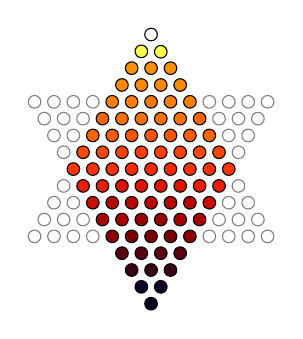
\begin{tikzpicture}
\filldraw [fill=C255] (0.000000,1.708957) circle (0.08); -- 57
\filldraw [fill=C207] (-0.123333,1.495337) circle (0.08); -- 46
\filldraw [fill=C207] (0.123333,1.490204) circle (0.08); -- 46
\filldraw [fill=C110] (-0.246667,1.281718) circle (0.08); -- 24
\filldraw [fill=C110] (0.000000,1.281718) circle (0.08); -- 24
\filldraw [fill=C110] (0.246667,1.281718) circle (0.08); -- 24
\filldraw [fill=C106] (-0.370000,1.068098) circle (0.08); -- 23
\filldraw [fill=C106] (-0.123333,1.068098) circle (0.08); -- 23
\filldraw [fill=C106] (0.123333,1.068098) circle (0.08); -- 23
\filldraw [fill=C106] (0.370000,1.068098) circle (0.08); -- 23
\draw [color=gray] (-1.480000,0.854478) circle (0.08); 
\draw [color=gray] (-1.233333,0.854478) circle (0.08); 
\draw [color=gray] (-0.986667,0.854478) circle (0.08); 
\draw [color=gray] (-0.740000,0.854478) circle (0.08); 
\filldraw [fill=C102] (-0.493333,0.854478) circle (0.08); -- 22
\filldraw [fill=C102] (-0.246667,0.854478) circle (0.08); -- 22
\filldraw [fill=C97] (0.000000,0.854478) circle (0.08); -- 21
\filldraw [fill=C102] (0.246667,0.854478) circle (0.08); -- 22
\filldraw [fill=C102] (0.493333,0.854478) circle (0.08); -- 22
\draw [color=gray] (0.740000,0.854478) circle (0.08); 
\draw [color=gray] (0.986667,0.854478) circle (0.08); 
\draw [color=gray] (1.233333,0.854478) circle (0.08); 
\draw [color=gray] (1.480000,0.854478) circle (0.08); 
\draw [color=gray] (-1.356667,0.640859) circle (0.08); 
\draw [color=gray] (-1.110000,0.640859) circle (0.08); 
\draw [color=gray] (-0.863333,0.640859) circle (0.08); 
\filldraw [fill=C88] (-0.616667,0.640859) circle (0.08); -- 19
\filldraw [fill=C93] (-0.370000,0.640859) circle (0.08); -- 20
\filldraw [fill=C93] (-0.123333,0.640859) circle (0.08); -- 20
\filldraw [fill=C93] (0.123333,0.640859) circle (0.08); -- 20
\filldraw [fill=C93] (0.370000,0.640859) circle (0.08); -- 20
\filldraw [fill=C88] (0.616667,0.640859) circle (0.08); -- 19
\draw [color=gray] (0.863333,0.640859) circle (0.08); 
\draw [color=gray] (1.110000,0.640859) circle (0.08); 
\draw [color=gray] (1.356667,0.640859) circle (0.08); 
\draw [color=gray] (-1.233333,0.427239) circle (0.08); 
\draw [color=gray] (-0.986667,0.427239) circle (0.08); 
\filldraw [fill=C88] (-0.740000,0.427239) circle (0.08); -- 19
\filldraw [fill=C84] (-0.493333,0.427239) circle (0.08); -- 18
\filldraw [fill=C80] (-0.246667,0.427239) circle (0.08); -- 17
\filldraw [fill=C80] (0.000000,0.427239) circle (0.08); -- 17
\filldraw [fill=C80] (0.246667,0.427239) circle (0.08); -- 17
\filldraw [fill=C84] (0.493333,0.427239) circle (0.08); -- 18
\filldraw [fill=C88] (0.740000,0.427239) circle (0.08); -- 19
\draw [color=gray] (0.986667,0.427239) circle (0.08); 
\draw [color=gray] (1.233333,0.427239) circle (0.08); 
\draw [color=gray] (-1.110000,0.213620) circle (0.08); 
\filldraw [fill=C75] (-0.863333,0.213620) circle (0.08); -- 16
\filldraw [fill=C75] (-0.616667,0.213620) circle (0.08); -- 16
\filldraw [fill=C71] (-0.370000,0.213620) circle (0.08); -- 15
\filldraw [fill=C71] (-0.123333,0.213620) circle (0.08); -- 15
\filldraw [fill=C71] (0.123333,0.213620) circle (0.08); -- 15
\filldraw [fill=C71] (0.370000,0.213620) circle (0.08); -- 15
\filldraw [fill=C75] (0.616667,0.213620) circle (0.08); -- 16
\filldraw [fill=C75] (0.863333,0.213620) circle (0.08); -- 16
\draw [color=gray] (1.110000,0.213620) circle (0.08); 
\filldraw [fill=C66] (-0.986667,0.000000) circle (0.08); -- 14
\filldraw [fill=C62] (-0.740000,0.000000) circle (0.08); -- 13
\filldraw [fill=C62] (-0.493333,0.000000) circle (0.08); -- 13
\filldraw [fill=C58] (-0.246667,0.000000) circle (0.08); -- 12
\filldraw [fill=C58] (0.000000,0.000000) circle (0.08); -- 12
\filldraw [fill=C58] (0.246667,0.000000) circle (0.08); -- 12
\filldraw [fill=C62] (0.493333,0.000000) circle (0.08); -- 13
\filldraw [fill=C62] (0.740000,0.000000) circle (0.08); -- 13
\filldraw [fill=C66] (0.986667,0.000000) circle (0.08); -- 14
\draw [color=gray] (-1.110000,-0.213620) circle (0.08); 
\filldraw [fill=C53] (-0.863333,-0.213620) circle (0.08); -- 11
\filldraw [fill=C53] (-0.616667,-0.213620) circle (0.08); -- 11
\filldraw [fill=C49] (-0.370000,-0.213620) circle (0.08); -- 10
\filldraw [fill=C49] (-0.123333,-0.213620) circle (0.08); -- 10
\filldraw [fill=C49] (0.123333,-0.213620) circle (0.08); -- 10
\filldraw [fill=C49] (0.370000,-0.213620) circle (0.08); -- 10
\filldraw [fill=C53] (0.616667,-0.213620) circle (0.08); -- 11
\filldraw [fill=C53] (0.863333,-0.213620) circle (0.08); -- 11
\draw [color=gray] (1.110000,-0.213620) circle (0.08); 
\draw [color=gray] (-1.233333,-0.427239) circle (0.08); 
\draw [color=gray] (-0.986667,-0.427239) circle (0.08); 
\filldraw [fill=C44] (-0.740000,-0.427239) circle (0.08); -- 9
\filldraw [fill=C40] (-0.493333,-0.427239) circle (0.08); -- 8
\filldraw [fill=C40] (-0.246667,-0.427239) circle (0.08); -- 8
\filldraw [fill=C40] (0.000000,-0.427239) circle (0.08); -- 8
\filldraw [fill=C40] (0.246667,-0.427239) circle (0.08); -- 8
\filldraw [fill=C40] (0.493333,-0.427239) circle (0.08); -- 8
\filldraw [fill=C44] (0.740000,-0.427239) circle (0.08); -- 9
\draw [color=gray] (0.986667,-0.427239) circle (0.08); 
\draw [color=gray] (1.233333,-0.427239) circle (0.08); 
\draw [color=gray] (-1.356667,-0.640859) circle (0.08); 
\draw [color=gray] (-1.110000,-0.640859) circle (0.08); 
\draw [color=gray] (-0.863333,-0.640859) circle (0.08); 
\filldraw [fill=C36] (-0.616667,-0.640859) circle (0.08); -- 7
\filldraw [fill=C36] (-0.370000,-0.640859) circle (0.08); -- 7
\filldraw [fill=C31] (-0.123333,-0.640859) circle (0.08); -- 6
\filldraw [fill=C31] (0.123333,-0.640859) circle (0.08); -- 6
\filldraw [fill=C36] (0.370000,-0.640859) circle (0.08); -- 7
\filldraw [fill=C36] (0.616667,-0.640859) circle (0.08); -- 7
\draw [color=gray] (0.863333,-0.640859) circle (0.08); 
\draw [color=gray] (1.110000,-0.640859) circle (0.08); 
\draw [color=gray] (1.356667,-0.640859) circle (0.08); 
\draw [color=gray] (-1.480000,-0.854478) circle (0.08); 
\draw [color=gray] (-1.233333,-0.854478) circle (0.08); 
\draw [color=gray] (-0.986667,-0.854478) circle (0.08); 
\draw [color=gray] (-0.740000,-0.854478) circle (0.08); 
\filldraw [fill=C27] (-0.493333,-0.854478) circle (0.08); -- 5
\filldraw [fill=C22] (-0.246667,-0.854478) circle (0.08); -- 4
\filldraw [fill=C22] (0.000000,-0.854478) circle (0.08); -- 4
\filldraw [fill=C22] (0.246667,-0.854478) circle (0.08); -- 4
\filldraw [fill=C27] (0.493333,-0.854478) circle (0.08); -- 5
\draw [color=gray] (0.740000,-0.854478) circle (0.08); 
\draw [color=gray] (0.986667,-0.854478) circle (0.08); 
\draw [color=gray] (1.233333,-0.854478) circle (0.08); 
\draw [color=gray] (1.480000,-0.854478) circle (0.08); 
\filldraw [fill=C18] (-0.370000,-1.068099) circle (0.08); -- 3
\filldraw [fill=C18] (-0.123333,-1.068099) circle (0.08); -- 3
\filldraw [fill=C18] (0.123333,-1.068099) circle (0.08); -- 3
\filldraw [fill=C18] (0.370000,-1.068099) circle (0.08); -- 3
\filldraw [fill=C14] (-0.246667,-1.281718) circle (0.08); -- 2
\filldraw [fill=C14] (0.000000,-1.281718) circle (0.08); -- 2
\filldraw [fill=C14] (0.246667,-1.281718) circle (0.08); -- 2
\filldraw [fill=C9] (-0.123333,-1.495338) circle (0.08); -- 1
\filldraw [fill=C9] (0.123333,-1.495338) circle (0.08); -- 1
\filldraw [fill=C5] (0.000000,-1.708957) circle (0.08); -- 0
\end{tikzpicture}

\caption{Our hand-tuned distance function. Pegs placed in the brighter
  positions give a lower score. Our bots use a search algorithm to
  find moves that place all pegs in the darkest positions, i.e.~it
  finds the moves that maximize the board evaluation function.}
\label{handtuned}
\end{figure}

The problem is that it's difficult to get a feel for how this function
acts when summed up over all pegs. Consider the case when the three
pegs at the top of the star are still in their starting position and
the seven other pegs are closer to the goal. There are two clusters of
pegs and if the board evaluation function has not been properly
designed then only the cluster closer to the goal will keep moving.
The cluster still in the starting position will only start moving
later in the game, when there are less opportunities for jumps.

The genetic algorithm that we used is shown in figure \ref{genalg}. It
never returns, but in our program it prints the most fit of each
generation. The algorithm is called with a population of (almost)
completely random individuals. To speed up the process the initial
individuals are not random in the start and goal positions. Figure
\ref{genpop0} shows a first-generation individual. The algorithm
measures the fitness of all individuals in the population and only the
most fit $20\%$ is kept. These individuals then mix to create a new
population with as many individuals as in the original population.
There is a $6.67\%$ chance that one of the new individuals will have
mutations. The mutations are guided so that it is less likely that
they will be detrimental.

The algorithm is not foolproof. Sometimes the surviving populations
are hopeless--they never start to have positive fitness values. If
that happens a new random population needs to be created.

\begin{figure}
\begin{algorithmic}
\Function{Genetic-Algorithm}{population, fitness-fn}
\While{$\top$}
 \State survivors = \textsc{Most-Fit}(population, fitness-fn, $1/5$)
 \State new-population = \emph{nil}
 \For{$\textrm{i} = 0 \to |\textrm{survivors}|$}
   \State x = \textsc{Random-Select}(survivors)
   \State y = \textsc{Random-Select}(survivors)
   \State child = \textsc{Reproduce}(x, y)
   \If{$\textsc{Random-Integer}(15)=0$}
     \State \textsc{Mutate}(child)
   \EndIf
   \State new-population[i] = child
 \EndFor
\EndWhile
\EndFunction
\\
\Function{Reproduce}{x, y}
\State z = \emph{nil}
\For{$\textrm{i} = 0 \to |\textrm{x}|$}
 \If{$\textsc{Random-Integer}(2) = 0$}
  \State z[i] = x[i]
 \Else
  \State z[i] = y[i]
 \EndIf
\EndFor
\State \Return z
\EndFunction
\\
\Function{Mutate}{x}
\State goal-positions = \emph{The positions in the player's goal}
\For{$\textrm{i} = 0 \to |\textrm{x}|$}
 \If{$\textsc{Random-Integer}(10) = 0$}
  \State $\textrm{v} = \textsc{Random-Integer}(50) - 25$
  \If{$\textrm{v} > 0 \vee \textrm{i} \in \textrm{goal-positions}$}
    \State x[i] = v
  \EndIf
 \EndIf
\EndFor
\ForAll{$\textrm{i} \in \textrm{goal-positions}$}
 \State x[i] = $\textsc{Min}(\textrm{x}[\textrm{i}], 5)$
\EndFor
\EndFunction
\end{algorithmic}

\caption{The genetic algorithm we used to derive a better board
  evaluation function. It is losely based on an algorithm from
  \cite{aimodern}.}
\label{genalg}
\end{figure}

The fitness function is the key to this genetic algorithm. Figure
\ref{fitness} shows that the early generations are not very successful
at all. Then after a while some individuals start winning games and
the general fitness of their offspring increases dramatically. Figure
\ref{winning} shows the rate at which the populations win. Our fitness
function is shown in figure \ref{fitnessfn}.

The \textsc{Simulation} function runs a game between two bots. In our
case it runs the generated bot against our hand-tuned bot. Both bots
are using a trivial search function that merely sorts all available
moves by the board evaluation function and does no lookahead. If we
used a more advanced search algorithm it would take much longer to run
the genetic algorithm, and we do not have the computing resources
required for that. Individuals from the early generations are likely
going to leave some pegs behind in the starting position, which
prevents either player from winning. In this case the simulation is
restarted.

The fitness function runs two simulations per individual and averages
the score. This gives an adequate and fast estimate for the early
generations. Later when the fitness function detects that the
individual is good at winning (it has an aggregate score over $300$)
it will switch over to running five simulations. This gives more
accurate estimates of an individual's fitness and decreases the
likelihood that a good individual will be penalized for what can be
considered as bad luck.

If the individual wins a simulation it is awarded $500-p$ points,
where $p$ is how many plies it needed to win. If it loses it is
penalized with $d$ points, where $d$ is a measure of how far away it
was from winning. This is computed using the same board evaluation
function that drives the bot used in the simulation. Thusly when the
bot populations are losing, they will try to be as close to winning as
possible. Later when they are winning they will be trying to win with
as few plies as possible.

\begin{figure}
\begin{algorithmic}
\Function{Fitness}{individual}
\State score = 0
\State iteration = 0
\While{$\top$}
 \If{$\textrm{iterations} = 2 \wedge \textrm{score} < 300$}
   \State \Return $\textrm{score} / 2$
 \ElsIf{$\textrm{iterations} = 5$}
   \State \Return $\textrm{score} / 5$
 \EndIf
 \State $\textrm{winner}, \textrm{plies}, \textrm{distance} = \textsc{Simulation}(\textrm{individual})$
 \If{$\textrm{winner} = \textrm{individual}$}
   \State $\textrm{score} = \textrm{score} + (500 - \textrm{plies})$
 \Else
   \State $\textrm{score} = \textrm{score} - \textrm{distance}$
 \EndIf
\EndWhile
\EndFunction
\end{algorithmic}
\caption{The fitness function computes a fitness score for an
  individual by having it play against a pre-defined bot.}
\label{fitnessfn}
\end{figure}


\begin{figure}
\centering
\includegraphics{population-fitness.pdf}
\caption{The fitness of the populations generated by the genetic
  algorithm improves over time. A lost game gives a negative fitness
  which gets closer to zero the closer the individual was to winning.
  Positive fitness means the game was won. The fewer moves were
  used, the higher the fitness becomes.}
\label{fitness}
\end{figure}

\begin{figure}
\centering
\includegraphics{population-winning-percentage.pdf}
\caption{The percentage of games won by the populations generated by
  the genetic algorithm.}
\label{winning}
\end{figure}

Figures \ref{genpop0}, \ref{genpop51}, \ref{genpop2427} and
\ref{genpop7822} show distance functions from different generations.
The first and second functions are not very useful in themselves, but
provide a point of comparison. It is interesting to note that in the
latter generations the genetic algorithm has built a path of darker
positions leading up the goal. Another noteworthy point is the darker
position in the lower right corner. There does not appear to be any
benefit to having a peg in this position. This is most likely an
artifact caused by the fitness function we used: in most two-player
games it is unlikely that there will be a peg in this position, so
there has been no evolutionary pressure to make this position lighter.
This will be bad in games with more than two players.

The genetic algorithm is easily adapted to simulate games between
three players. Figure \ref{gen3pop3594} shows an individual from such
a simulation. It is remarkably similar to the two-player individual
from figure \ref{genpop7822}. A three-player game exercises more of
the positions on the board and therefore places greater demands on the
individual. The dark positions are no longer isolated from the rest of
the board: they are connected to the goal by some path. Running
simulations with three players not only requires more CPU time, but
also requires more generations before it gets good results (figures
\ref{fitness} and \ref{winning}). The results for four players were
promising, but could not be completed due to lack of time. Games with
more than four players have not been attempted.

\begin{figure}
\centering
\definecolor{C0}{rgb}{0.000000,0.000000,0.000000}
\definecolor{C1}{rgb}{0.000000,0.000000,0.094118}
\definecolor{C2}{rgb}{0.000000,0.000000,0.094118}
\definecolor{C3}{rgb}{0.000000,0.000000,0.109804}
\definecolor{C4}{rgb}{0.000000,0.000000,0.125490}
\definecolor{C5}{rgb}{0.000000,0.000000,0.125490}
\definecolor{C6}{rgb}{0.000000,0.000000,0.141176}
\definecolor{C7}{rgb}{0.000000,0.000000,0.156863}
\definecolor{C8}{rgb}{0.031373,0.000000,0.156863}
\definecolor{C9}{rgb}{0.062745,0.000000,0.141176}
\definecolor{C10}{rgb}{0.094118,0.000000,0.141176}
\definecolor{C11}{rgb}{0.125490,0.000000,0.125490}
\definecolor{C12}{rgb}{0.156863,0.000000,0.109804}
\definecolor{C13}{rgb}{0.188235,0.000000,0.109804}
\definecolor{C14}{rgb}{0.219608,0.000000,0.094118}
\definecolor{C15}{rgb}{0.250980,0.000000,0.078431}
\definecolor{C16}{rgb}{0.282353,0.000000,0.078431}
\definecolor{C17}{rgb}{0.313725,0.000000,0.062745}
\definecolor{C18}{rgb}{0.345098,0.000000,0.062745}
\definecolor{C19}{rgb}{0.376471,0.000000,0.047059}
\definecolor{C20}{rgb}{0.407843,0.000000,0.031373}
\definecolor{C21}{rgb}{0.439216,0.000000,0.031373}
\definecolor{C22}{rgb}{0.470588,0.000000,0.015686}
\definecolor{C23}{rgb}{0.501961,0.000000,0.000000}
\definecolor{C24}{rgb}{0.501961,0.000000,0.000000}
\definecolor{C25}{rgb}{0.517647,0.000000,0.000000}
\definecolor{C26}{rgb}{0.533333,0.000000,0.000000}
\definecolor{C27}{rgb}{0.549020,0.000000,0.000000}
\definecolor{C28}{rgb}{0.564706,0.000000,0.000000}
\definecolor{C29}{rgb}{0.564706,0.000000,0.000000}
\definecolor{C30}{rgb}{0.580392,0.000000,0.000000}
\definecolor{C31}{rgb}{0.596078,0.000000,0.000000}
\definecolor{C32}{rgb}{0.611765,0.000000,0.000000}
\definecolor{C33}{rgb}{0.627451,0.000000,0.000000}
\definecolor{C34}{rgb}{0.627451,0.000000,0.000000}
\definecolor{C35}{rgb}{0.643137,0.000000,0.000000}
\definecolor{C36}{rgb}{0.658824,0.000000,0.000000}
\definecolor{C37}{rgb}{0.674510,0.000000,0.000000}
\definecolor{C38}{rgb}{0.690196,0.000000,0.000000}
\definecolor{C39}{rgb}{0.705882,0.000000,0.000000}
\definecolor{C40}{rgb}{0.721569,0.015686,0.000000}
\definecolor{C41}{rgb}{0.737255,0.015686,0.000000}
\definecolor{C42}{rgb}{0.752941,0.031373,0.000000}
\definecolor{C43}{rgb}{0.768627,0.031373,0.000000}
\definecolor{C44}{rgb}{0.784314,0.047059,0.000000}
\definecolor{C45}{rgb}{0.800000,0.047059,0.000000}
\definecolor{C46}{rgb}{0.815686,0.062745,0.000000}
\definecolor{C47}{rgb}{0.831373,0.062745,0.000000}
\definecolor{C48}{rgb}{0.847059,0.078431,0.000000}
\definecolor{C49}{rgb}{0.862745,0.078431,0.000000}
\definecolor{C50}{rgb}{0.878431,0.094118,0.000000}
\definecolor{C51}{rgb}{0.894118,0.094118,0.000000}
\definecolor{C52}{rgb}{0.909804,0.109804,0.000000}
\definecolor{C53}{rgb}{0.925490,0.109804,0.000000}
\definecolor{C54}{rgb}{0.941176,0.125490,0.000000}
\definecolor{C55}{rgb}{0.956863,0.125490,0.000000}
\definecolor{C56}{rgb}{0.988235,0.141176,0.000000}
\definecolor{C57}{rgb}{0.988235,0.141176,0.000000}
\definecolor{C58}{rgb}{0.988235,0.156863,0.000000}
\definecolor{C59}{rgb}{0.988235,0.156863,0.000000}
\definecolor{C60}{rgb}{0.988235,0.172549,0.000000}
\definecolor{C61}{rgb}{0.988235,0.172549,0.000000}
\definecolor{C62}{rgb}{0.988235,0.188235,0.000000}
\definecolor{C63}{rgb}{0.988235,0.188235,0.000000}
\definecolor{C64}{rgb}{0.988235,0.203922,0.000000}
\definecolor{C65}{rgb}{0.988235,0.203922,0.000000}
\definecolor{C66}{rgb}{0.988235,0.219608,0.000000}
\definecolor{C67}{rgb}{0.988235,0.219608,0.000000}
\definecolor{C68}{rgb}{0.988235,0.235294,0.000000}
\definecolor{C69}{rgb}{0.988235,0.235294,0.000000}
\definecolor{C70}{rgb}{0.988235,0.250980,0.000000}
\definecolor{C71}{rgb}{0.988235,0.250980,0.000000}
\definecolor{C72}{rgb}{0.988235,0.266667,0.000000}
\definecolor{C73}{rgb}{0.988235,0.266667,0.000000}
\definecolor{C74}{rgb}{0.988235,0.282353,0.000000}
\definecolor{C75}{rgb}{0.988235,0.282353,0.000000}
\definecolor{C76}{rgb}{0.988235,0.298039,0.000000}
\definecolor{C77}{rgb}{0.988235,0.298039,0.000000}
\definecolor{C78}{rgb}{0.988235,0.313725,0.000000}
\definecolor{C79}{rgb}{0.988235,0.313725,0.000000}
\definecolor{C80}{rgb}{0.988235,0.329412,0.000000}
\definecolor{C81}{rgb}{0.988235,0.329412,0.000000}
\definecolor{C82}{rgb}{0.988235,0.345098,0.000000}
\definecolor{C83}{rgb}{0.988235,0.345098,0.000000}
\definecolor{C84}{rgb}{0.988235,0.360784,0.000000}
\definecolor{C85}{rgb}{0.988235,0.376471,0.000000}
\definecolor{C86}{rgb}{0.988235,0.376471,0.000000}
\definecolor{C87}{rgb}{0.988235,0.392157,0.000000}
\definecolor{C88}{rgb}{0.988235,0.392157,0.000000}
\definecolor{C89}{rgb}{0.988235,0.407843,0.000000}
\definecolor{C90}{rgb}{0.988235,0.407843,0.000000}
\definecolor{C91}{rgb}{0.988235,0.423529,0.000000}
\definecolor{C92}{rgb}{0.988235,0.423529,0.000000}
\definecolor{C93}{rgb}{0.988235,0.439216,0.000000}
\definecolor{C94}{rgb}{0.988235,0.439216,0.000000}
\definecolor{C95}{rgb}{0.988235,0.454902,0.000000}
\definecolor{C96}{rgb}{0.988235,0.454902,0.000000}
\definecolor{C97}{rgb}{0.988235,0.470588,0.000000}
\definecolor{C98}{rgb}{0.988235,0.470588,0.000000}
\definecolor{C99}{rgb}{0.988235,0.486275,0.000000}
\definecolor{C100}{rgb}{0.988235,0.486275,0.000000}
\definecolor{C101}{rgb}{0.988235,0.501961,0.000000}
\definecolor{C102}{rgb}{0.988235,0.501961,0.000000}
\definecolor{C103}{rgb}{0.988235,0.517647,0.000000}
\definecolor{C104}{rgb}{0.988235,0.517647,0.000000}
\definecolor{C105}{rgb}{0.988235,0.533333,0.000000}
\definecolor{C106}{rgb}{0.988235,0.533333,0.000000}
\definecolor{C107}{rgb}{0.988235,0.549020,0.000000}
\definecolor{C108}{rgb}{0.988235,0.549020,0.000000}
\definecolor{C109}{rgb}{0.988235,0.564706,0.000000}
\definecolor{C110}{rgb}{0.988235,0.564706,0.000000}
\definecolor{C111}{rgb}{0.988235,0.580392,0.000000}
\definecolor{C112}{rgb}{0.988235,0.596078,0.000000}
\definecolor{C113}{rgb}{0.988235,0.596078,0.000000}
\definecolor{C114}{rgb}{0.988235,0.611765,0.000000}
\definecolor{C115}{rgb}{0.988235,0.611765,0.000000}
\definecolor{C116}{rgb}{0.988235,0.627451,0.000000}
\definecolor{C117}{rgb}{0.988235,0.627451,0.000000}
\definecolor{C118}{rgb}{0.988235,0.643137,0.000000}
\definecolor{C119}{rgb}{0.988235,0.643137,0.000000}
\definecolor{C120}{rgb}{0.988235,0.658824,0.000000}
\definecolor{C121}{rgb}{0.988235,0.658824,0.000000}
\definecolor{C122}{rgb}{0.988235,0.674510,0.000000}
\definecolor{C123}{rgb}{0.988235,0.674510,0.000000}
\definecolor{C124}{rgb}{0.988235,0.690196,0.000000}
\definecolor{C125}{rgb}{0.988235,0.690196,0.000000}
\definecolor{C126}{rgb}{0.988235,0.705882,0.000000}
\definecolor{C127}{rgb}{0.988235,0.705882,0.000000}
\definecolor{C128}{rgb}{0.988235,0.721569,0.000000}
\definecolor{C129}{rgb}{0.988235,0.721569,0.000000}
\definecolor{C130}{rgb}{0.988235,0.737255,0.000000}
\definecolor{C131}{rgb}{0.988235,0.737255,0.000000}
\definecolor{C132}{rgb}{0.988235,0.752941,0.000000}
\definecolor{C133}{rgb}{0.988235,0.752941,0.000000}
\definecolor{C134}{rgb}{0.988235,0.768627,0.000000}
\definecolor{C135}{rgb}{0.988235,0.768627,0.000000}
\definecolor{C136}{rgb}{0.988235,0.784314,0.000000}
\definecolor{C137}{rgb}{0.988235,0.784314,0.000000}
\definecolor{C138}{rgb}{0.988235,0.800000,0.000000}
\definecolor{C139}{rgb}{0.988235,0.815686,0.000000}
\definecolor{C140}{rgb}{0.988235,0.815686,0.000000}
\definecolor{C141}{rgb}{0.988235,0.815686,0.000000}
\definecolor{C142}{rgb}{0.988235,0.815686,0.000000}
\definecolor{C143}{rgb}{0.988235,0.815686,0.000000}
\definecolor{C144}{rgb}{0.988235,0.831373,0.000000}
\definecolor{C145}{rgb}{0.988235,0.831373,0.000000}
\definecolor{C146}{rgb}{0.988235,0.831373,0.000000}
\definecolor{C147}{rgb}{0.988235,0.831373,0.000000}
\definecolor{C148}{rgb}{0.988235,0.847059,0.000000}
\definecolor{C149}{rgb}{0.988235,0.847059,0.000000}
\definecolor{C150}{rgb}{0.988235,0.847059,0.000000}
\definecolor{C151}{rgb}{0.988235,0.847059,0.000000}
\definecolor{C152}{rgb}{0.988235,0.847059,0.000000}
\definecolor{C153}{rgb}{0.988235,0.862745,0.000000}
\definecolor{C154}{rgb}{0.988235,0.862745,0.000000}
\definecolor{C155}{rgb}{0.988235,0.862745,0.000000}
\definecolor{C156}{rgb}{0.988235,0.862745,0.000000}
\definecolor{C157}{rgb}{0.988235,0.878431,0.000000}
\definecolor{C158}{rgb}{0.988235,0.878431,0.000000}
\definecolor{C159}{rgb}{0.988235,0.878431,0.000000}
\definecolor{C160}{rgb}{0.988235,0.878431,0.000000}
\definecolor{C161}{rgb}{0.988235,0.894118,0.000000}
\definecolor{C162}{rgb}{0.988235,0.894118,0.000000}
\definecolor{C163}{rgb}{0.988235,0.894118,0.000000}
\definecolor{C164}{rgb}{0.988235,0.894118,0.000000}
\definecolor{C165}{rgb}{0.988235,0.894118,0.000000}
\definecolor{C166}{rgb}{0.988235,0.909804,0.000000}
\definecolor{C167}{rgb}{0.988235,0.909804,0.000000}
\definecolor{C168}{rgb}{0.988235,0.909804,0.000000}
\definecolor{C169}{rgb}{0.988235,0.909804,0.000000}
\definecolor{C170}{rgb}{0.988235,0.925490,0.000000}
\definecolor{C171}{rgb}{0.988235,0.925490,0.000000}
\definecolor{C172}{rgb}{0.988235,0.925490,0.000000}
\definecolor{C173}{rgb}{0.988235,0.925490,0.000000}
\definecolor{C174}{rgb}{0.988235,0.941176,0.000000}
\definecolor{C175}{rgb}{0.988235,0.941176,0.000000}
\definecolor{C176}{rgb}{0.988235,0.941176,0.000000}
\definecolor{C177}{rgb}{0.988235,0.941176,0.000000}
\definecolor{C178}{rgb}{0.988235,0.941176,0.000000}
\definecolor{C179}{rgb}{0.988235,0.956863,0.000000}
\definecolor{C180}{rgb}{0.988235,0.956863,0.000000}
\definecolor{C181}{rgb}{0.988235,0.956863,0.000000}
\definecolor{C182}{rgb}{0.988235,0.956863,0.000000}
\definecolor{C183}{rgb}{0.988235,0.972549,0.000000}
\definecolor{C184}{rgb}{0.988235,0.972549,0.000000}
\definecolor{C185}{rgb}{0.988235,0.972549,0.000000}
\definecolor{C186}{rgb}{0.988235,0.972549,0.000000}
\definecolor{C187}{rgb}{0.988235,0.988235,0.000000}
\definecolor{C188}{rgb}{0.988235,0.988235,0.015686}
\definecolor{C189}{rgb}{0.988235,0.988235,0.031373}
\definecolor{C190}{rgb}{0.988235,0.988235,0.047059}
\definecolor{C191}{rgb}{0.988235,0.988235,0.062745}
\definecolor{C192}{rgb}{0.988235,0.988235,0.078431}
\definecolor{C193}{rgb}{0.988235,0.988235,0.094118}
\definecolor{C194}{rgb}{0.988235,0.988235,0.109804}
\definecolor{C195}{rgb}{0.988235,0.988235,0.125490}
\definecolor{C196}{rgb}{0.988235,0.988235,0.141176}
\definecolor{C197}{rgb}{0.988235,0.988235,0.156863}
\definecolor{C198}{rgb}{0.988235,0.988235,0.156863}
\definecolor{C199}{rgb}{0.988235,0.988235,0.172549}
\definecolor{C200}{rgb}{0.988235,0.988235,0.188235}
\definecolor{C201}{rgb}{0.988235,0.988235,0.203922}
\definecolor{C202}{rgb}{0.988235,0.988235,0.219608}
\definecolor{C203}{rgb}{0.988235,0.988235,0.235294}
\definecolor{C204}{rgb}{0.988235,0.988235,0.250980}
\definecolor{C205}{rgb}{0.988235,0.988235,0.266667}
\definecolor{C206}{rgb}{0.988235,0.988235,0.282353}
\definecolor{C207}{rgb}{0.988235,0.988235,0.298039}
\definecolor{C208}{rgb}{0.988235,0.988235,0.313725}
\definecolor{C209}{rgb}{0.988235,0.988235,0.329412}
\definecolor{C210}{rgb}{0.988235,0.988235,0.329412}
\definecolor{C211}{rgb}{0.988235,0.988235,0.345098}
\definecolor{C212}{rgb}{0.988235,0.988235,0.360784}
\definecolor{C213}{rgb}{0.988235,0.988235,0.376471}
\definecolor{C214}{rgb}{0.988235,0.988235,0.392157}
\definecolor{C215}{rgb}{0.988235,0.988235,0.407843}
\definecolor{C216}{rgb}{0.988235,0.988235,0.423529}
\definecolor{C217}{rgb}{0.988235,0.988235,0.439216}
\definecolor{C218}{rgb}{0.988235,0.988235,0.454902}
\definecolor{C219}{rgb}{0.988235,0.988235,0.470588}
\definecolor{C220}{rgb}{0.988235,0.988235,0.486275}
\definecolor{C221}{rgb}{0.988235,0.988235,0.486275}
\definecolor{C222}{rgb}{0.988235,0.988235,0.501961}
\definecolor{C223}{rgb}{0.988235,0.988235,0.517647}
\definecolor{C224}{rgb}{0.988235,0.988235,0.533333}
\definecolor{C225}{rgb}{0.988235,0.988235,0.549020}
\definecolor{C226}{rgb}{0.988235,0.988235,0.564706}
\definecolor{C227}{rgb}{0.988235,0.988235,0.580392}
\definecolor{C228}{rgb}{0.988235,0.988235,0.596078}
\definecolor{C229}{rgb}{0.988235,0.988235,0.611765}
\definecolor{C230}{rgb}{0.988235,0.988235,0.627451}
\definecolor{C231}{rgb}{0.988235,0.988235,0.643137}
\definecolor{C232}{rgb}{0.988235,0.988235,0.658824}
\definecolor{C233}{rgb}{0.988235,0.988235,0.658824}
\definecolor{C234}{rgb}{0.988235,0.988235,0.674510}
\definecolor{C235}{rgb}{0.988235,0.988235,0.690196}
\definecolor{C236}{rgb}{0.988235,0.988235,0.705882}
\definecolor{C237}{rgb}{0.988235,0.988235,0.721569}
\definecolor{C238}{rgb}{0.988235,0.988235,0.737255}
\definecolor{C239}{rgb}{0.988235,0.988235,0.752941}
\definecolor{C240}{rgb}{0.988235,0.988235,0.768627}
\definecolor{C241}{rgb}{0.988235,0.988235,0.784314}
\definecolor{C242}{rgb}{0.988235,0.988235,0.800000}
\definecolor{C243}{rgb}{0.988235,0.988235,0.815686}
\definecolor{C244}{rgb}{0.988235,0.988235,0.815686}
\definecolor{C245}{rgb}{0.988235,0.988235,0.831373}
\definecolor{C246}{rgb}{0.988235,0.988235,0.847059}
\definecolor{C247}{rgb}{0.988235,0.988235,0.862745}
\definecolor{C248}{rgb}{0.988235,0.988235,0.878431}
\definecolor{C249}{rgb}{0.988235,0.988235,0.894118}
\definecolor{C250}{rgb}{0.988235,0.988235,0.909804}
\definecolor{C251}{rgb}{0.988235,0.988235,0.925490}
\definecolor{C252}{rgb}{0.988235,0.988235,0.941176}
\definecolor{C253}{rgb}{0.988235,0.988235,0.956863}
\definecolor{C254}{rgb}{0.988235,0.988235,0.972549}
\definecolor{C255}{rgb}{0.988235,0.988235,0.988235}

%% vec = (151, 77, 136, 115, 500, 119, 153, 32, 128, 184, 44, 156, 89, 147, 115, 29, 77, 121, 102, 31, 31, 500, 500, 17, 172, 11, 130, 77, 148, 39, 153, 100, 117, 89, 15, 117, 9, 168, 200, 200, 200, 193, 94, 42, 140, 10, 72, 17, 132, 174, 49, 163, 17, 143, 181, 200, 200, 200, 200, 104, 152, 20, 4, 69, 110, 19, 187, 119, 188, 136, 57, 141, 130, 152, 183, 71, 163, 55, 88, 95, 30, 138, 59, 48, 82, 40, 37, 37, 153, 104, 141, 105, 124, 146, 174, 35, 165, 161, 155, 154, 98, 12, 95, 28, 165, 79, 99, 128, 134, 188, 24, 165, 127, 83, 13, 9, 124, 51, 47, 78, 155, 188, 183, 80, 134, 158, 115, 100, 120, 70, 54, 18, 83, 150, 47, 48, 29, 147, 177, 164, 136, 1, 129, 63, 85, 143, 73, 10, 194, 120, 89, 149, 108, 72, 29, 43, 30, 145, 144, 151, 16, 199, 170, 99, 149, 17, 148, 178, 165, 125, 142, 101, 127, 72, 165, 13, 15, 38, 24, 9, 159, 113, 159, 68, 186, 189, 111, 17, 134, 56, 168, 150, 55, 138, 50, 4, 156, 198, 183, 121, 124, 126, 23, 52, 198, 188, 65, 14, 27, 90, 23, 186, 3, 182, 54, 190, 171, 166, 7, 106, 22, 175, 57, 77, 114, 107, 82, 70, 105, 66, 0, 0, 0, 0, 82, 191, 4, 147, 5, 31, 38, 28, 18, 42, 11, 73, 32, 183, 0, 0, 0, 62, 15, 147, 140, 129, 54, 23, 199, 160, 89, 191, 190, 81, 6, 72, 0, 0, 20, 77, 42, 58, 106, 61, 101, 118, 134, 133, 101, 174, 172, 191, 37, 188, 0, 177, 117, 193, 0)
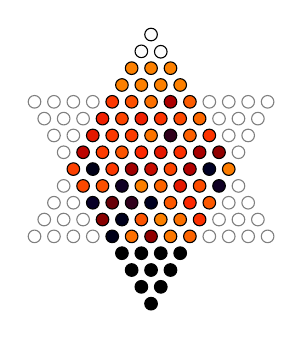
\begin{tikzpicture}
\filldraw [fill=C255] (0.000000,1.708957) circle (0.08); -- 500
\filldraw [fill=C255] (-0.123333,1.495337) circle (0.08); -- 500
\filldraw [fill=C255] (0.123333,1.490204) circle (0.08); -- 500
\filldraw [fill=C102] (-0.246667,1.281718) circle (0.08); -- 200
\filldraw [fill=C102] (0.000000,1.281718) circle (0.08); -- 200
\filldraw [fill=C102] (0.246667,1.281718) circle (0.08); -- 200
\filldraw [fill=C102] (-0.370000,1.068098) circle (0.08); -- 200
\filldraw [fill=C102] (-0.123333,1.068098) circle (0.08); -- 200
\filldraw [fill=C102] (0.123333,1.068098) circle (0.08); -- 200
\filldraw [fill=C102] (0.370000,1.068098) circle (0.08); -- 200
\draw [color=gray] (-1.480000,0.854478) circle (0.08); 
\draw [color=gray] (-1.233333,0.854478) circle (0.08); 
\draw [color=gray] (-0.986667,0.854478) circle (0.08); 
\draw [color=gray] (-0.740000,0.854478) circle (0.08); 
\filldraw [fill=C67] (-0.493333,0.854478) circle (0.08); -- 130
\filldraw [fill=C78] (-0.246667,0.854478) circle (0.08); -- 152
\filldraw [fill=C94] (0.000000,0.854478) circle (0.08); -- 183
\filldraw [fill=C37] (0.246667,0.854478) circle (0.08); -- 71
\filldraw [fill=C84] (0.493333,0.854478) circle (0.08); -- 163
\draw [color=gray] (0.740000,0.854478) circle (0.08); 
\draw [color=gray] (0.986667,0.854478) circle (0.08); 
\draw [color=gray] (1.233333,0.854478) circle (0.08); 
\draw [color=gray] (1.480000,0.854478) circle (0.08); 
\draw [color=gray] (-1.356667,0.640859) circle (0.08); 
\draw [color=gray] (-1.110000,0.640859) circle (0.08); 
\draw [color=gray] (-0.863333,0.640859) circle (0.08); 
\filldraw [fill=C54] (-0.616667,0.640859) circle (0.08); -- 104
\filldraw [fill=C72] (-0.370000,0.640859) circle (0.08); -- 141
\filldraw [fill=C54] (-0.123333,0.640859) circle (0.08); -- 105
\filldraw [fill=C64] (0.123333,0.640859) circle (0.08); -- 124
\filldraw [fill=C75] (0.370000,0.640859) circle (0.08); -- 146
\filldraw [fill=C89] (0.616667,0.640859) circle (0.08); -- 174
\draw [color=gray] (0.863333,0.640859) circle (0.08); 
\draw [color=gray] (1.110000,0.640859) circle (0.08); 
\draw [color=gray] (1.356667,0.640859) circle (0.08); 
\draw [color=gray] (-1.233333,0.427239) circle (0.08); 
\draw [color=gray] (-0.986667,0.427239) circle (0.08); 
\filldraw [fill=C51] (-0.740000,0.427239) circle (0.08); -- 99
\filldraw [fill=C66] (-0.493333,0.427239) circle (0.08); -- 128
\filldraw [fill=C69] (-0.246667,0.427239) circle (0.08); -- 134
\filldraw [fill=C96] (0.000000,0.427239) circle (0.08); -- 188
\filldraw [fill=C13] (0.246667,0.427239) circle (0.08); -- 24
\filldraw [fill=C85] (0.493333,0.427239) circle (0.08); -- 165
\filldraw [fill=C65] (0.740000,0.427239) circle (0.08); -- 127
\draw [color=gray] (0.986667,0.427239) circle (0.08); 
\draw [color=gray] (1.233333,0.427239) circle (0.08); 
\draw [color=gray] (-1.110000,0.213620) circle (0.08); 
\filldraw [fill=C41] (-0.863333,0.213620) circle (0.08); -- 80
\filldraw [fill=C69] (-0.616667,0.213620) circle (0.08); -- 134
\filldraw [fill=C81] (-0.370000,0.213620) circle (0.08); -- 158
\filldraw [fill=C59] (-0.123333,0.213620) circle (0.08); -- 115
\filldraw [fill=C51] (0.123333,0.213620) circle (0.08); -- 100
\filldraw [fill=C62] (0.370000,0.213620) circle (0.08); -- 120
\filldraw [fill=C36] (0.616667,0.213620) circle (0.08); -- 70
\filldraw [fill=C28] (0.863333,0.213620) circle (0.08); -- 54
\draw [color=gray] (1.110000,0.213620) circle (0.08); 
\filldraw [fill=C70] (-0.986667,0.000000) circle (0.08); -- 136
\filldraw [fill=C1] (-0.740000,0.000000) circle (0.08); -- 1
\filldraw [fill=C66] (-0.493333,0.000000) circle (0.08); -- 129
\filldraw [fill=C33] (-0.246667,0.000000) circle (0.08); -- 63
\filldraw [fill=C44] (0.000000,0.000000) circle (0.08); -- 85
\filldraw [fill=C73] (0.246667,0.000000) circle (0.08); -- 143
\filldraw [fill=C38] (0.493333,0.000000) circle (0.08); -- 73
\filldraw [fill=C6] (0.740000,0.000000) circle (0.08); -- 10
\filldraw [fill=C99] (0.986667,0.000000) circle (0.08); -- 194
\draw [color=gray] (-1.110000,-0.213620) circle (0.08); 
\filldraw [fill=C74] (-0.863333,-0.213620) circle (0.08); -- 144
\filldraw [fill=C78] (-0.616667,-0.213620) circle (0.08); -- 151
\filldraw [fill=C9] (-0.370000,-0.213620) circle (0.08); -- 16
\filldraw [fill=C102] (-0.123333,-0.213620) circle (0.08); -- 199
\filldraw [fill=C87] (0.123333,-0.213620) circle (0.08); -- 170
\filldraw [fill=C51] (0.370000,-0.213620) circle (0.08); -- 99
\filldraw [fill=C76] (0.616667,-0.213620) circle (0.08); -- 149
\filldraw [fill=C9] (0.863333,-0.213620) circle (0.08); -- 17
\draw [color=gray] (1.110000,-0.213620) circle (0.08); 
\draw [color=gray] (-1.233333,-0.427239) circle (0.08); 
\draw [color=gray] (-0.986667,-0.427239) circle (0.08); 
\filldraw [fill=C8] (-0.740000,-0.427239) circle (0.08); -- 15
\filldraw [fill=C20] (-0.493333,-0.427239) circle (0.08); -- 38
\filldraw [fill=C13] (-0.246667,-0.427239) circle (0.08); -- 24
\filldraw [fill=C5] (0.000000,-0.427239) circle (0.08); -- 9
\filldraw [fill=C82] (0.246667,-0.427239) circle (0.08); -- 159
\filldraw [fill=C58] (0.493333,-0.427239) circle (0.08); -- 113
\filldraw [fill=C82] (0.740000,-0.427239) circle (0.08); -- 159
\draw [color=gray] (0.986667,-0.427239) circle (0.08); 
\draw [color=gray] (1.233333,-0.427239) circle (0.08); 
\draw [color=gray] (-1.356667,-0.640859) circle (0.08); 
\draw [color=gray] (-1.110000,-0.640859) circle (0.08); 
\draw [color=gray] (-0.863333,-0.640859) circle (0.08); 
\filldraw [fill=C26] (-0.616667,-0.640859) circle (0.08); -- 50
\filldraw [fill=C3] (-0.370000,-0.640859) circle (0.08); -- 4
\filldraw [fill=C80] (-0.123333,-0.640859) circle (0.08); -- 156
\filldraw [fill=C101] (0.123333,-0.640859) circle (0.08); -- 198
\filldraw [fill=C94] (0.370000,-0.640859) circle (0.08); -- 183
\filldraw [fill=C62] (0.616667,-0.640859) circle (0.08); -- 121
\draw [color=gray] (0.863333,-0.640859) circle (0.08); 
\draw [color=gray] (1.110000,-0.640859) circle (0.08); 
\draw [color=gray] (1.356667,-0.640859) circle (0.08); 
\draw [color=gray] (-1.480000,-0.854478) circle (0.08); 
\draw [color=gray] (-1.233333,-0.854478) circle (0.08); 
\draw [color=gray] (-0.986667,-0.854478) circle (0.08); 
\draw [color=gray] (-0.740000,-0.854478) circle (0.08); 
\filldraw [fill=C2] (-0.493333,-0.854478) circle (0.08); -- 3
\filldraw [fill=C93] (-0.246667,-0.854478) circle (0.08); -- 182
\filldraw [fill=C28] (0.000000,-0.854478) circle (0.08); -- 54
\filldraw [fill=C97] (0.246667,-0.854478) circle (0.08); -- 190
\filldraw [fill=C88] (0.493333,-0.854478) circle (0.08); -- 171
\draw [color=gray] (0.740000,-0.854478) circle (0.08); 
\draw [color=gray] (0.986667,-0.854478) circle (0.08); 
\draw [color=gray] (1.233333,-0.854478) circle (0.08); 
\draw [color=gray] (1.480000,-0.854478) circle (0.08); 
\filldraw [fill=C0] (-0.370000,-1.068099) circle (0.08); -- 0
\filldraw [fill=C0] (-0.123333,-1.068099) circle (0.08); -- 0
\filldraw [fill=C0] (0.123333,-1.068099) circle (0.08); -- 0
\filldraw [fill=C0] (0.370000,-1.068099) circle (0.08); -- 0
\filldraw [fill=C0] (-0.246667,-1.281718) circle (0.08); -- 0
\filldraw [fill=C0] (0.000000,-1.281718) circle (0.08); -- 0
\filldraw [fill=C0] (0.246667,-1.281718) circle (0.08); -- 0
\filldraw [fill=C0] (-0.123333,-1.495338) circle (0.08); -- 0
\filldraw [fill=C0] (0.123333,-1.495338) circle (0.08); -- 0
\filldraw [fill=C0] (0.000000,-1.708957) circle (0.08); -- 0
\end{tikzpicture}

\caption{The most fit distance function at generation 0. The first
  generation is fully random except for the start and goal positions.
  This individual did not win any games at all.}
\label{genpop0}
\end{figure}

\begin{figure}
\centering
\definecolor{C0}{rgb}{0.000000,0.000000,0.000000}
\definecolor{C1}{rgb}{0.000000,0.000000,0.094118}
\definecolor{C2}{rgb}{0.000000,0.000000,0.094118}
\definecolor{C3}{rgb}{0.000000,0.000000,0.109804}
\definecolor{C4}{rgb}{0.000000,0.000000,0.125490}
\definecolor{C5}{rgb}{0.000000,0.000000,0.125490}
\definecolor{C6}{rgb}{0.000000,0.000000,0.141176}
\definecolor{C7}{rgb}{0.000000,0.000000,0.156863}
\definecolor{C8}{rgb}{0.031373,0.000000,0.156863}
\definecolor{C9}{rgb}{0.062745,0.000000,0.141176}
\definecolor{C10}{rgb}{0.094118,0.000000,0.141176}
\definecolor{C11}{rgb}{0.125490,0.000000,0.125490}
\definecolor{C12}{rgb}{0.156863,0.000000,0.109804}
\definecolor{C13}{rgb}{0.188235,0.000000,0.109804}
\definecolor{C14}{rgb}{0.219608,0.000000,0.094118}
\definecolor{C15}{rgb}{0.250980,0.000000,0.078431}
\definecolor{C16}{rgb}{0.282353,0.000000,0.078431}
\definecolor{C17}{rgb}{0.313725,0.000000,0.062745}
\definecolor{C18}{rgb}{0.345098,0.000000,0.062745}
\definecolor{C19}{rgb}{0.376471,0.000000,0.047059}
\definecolor{C20}{rgb}{0.407843,0.000000,0.031373}
\definecolor{C21}{rgb}{0.439216,0.000000,0.031373}
\definecolor{C22}{rgb}{0.470588,0.000000,0.015686}
\definecolor{C23}{rgb}{0.501961,0.000000,0.000000}
\definecolor{C24}{rgb}{0.501961,0.000000,0.000000}
\definecolor{C25}{rgb}{0.517647,0.000000,0.000000}
\definecolor{C26}{rgb}{0.533333,0.000000,0.000000}
\definecolor{C27}{rgb}{0.549020,0.000000,0.000000}
\definecolor{C28}{rgb}{0.564706,0.000000,0.000000}
\definecolor{C29}{rgb}{0.564706,0.000000,0.000000}
\definecolor{C30}{rgb}{0.580392,0.000000,0.000000}
\definecolor{C31}{rgb}{0.596078,0.000000,0.000000}
\definecolor{C32}{rgb}{0.611765,0.000000,0.000000}
\definecolor{C33}{rgb}{0.627451,0.000000,0.000000}
\definecolor{C34}{rgb}{0.627451,0.000000,0.000000}
\definecolor{C35}{rgb}{0.643137,0.000000,0.000000}
\definecolor{C36}{rgb}{0.658824,0.000000,0.000000}
\definecolor{C37}{rgb}{0.674510,0.000000,0.000000}
\definecolor{C38}{rgb}{0.690196,0.000000,0.000000}
\definecolor{C39}{rgb}{0.705882,0.000000,0.000000}
\definecolor{C40}{rgb}{0.721569,0.015686,0.000000}
\definecolor{C41}{rgb}{0.737255,0.015686,0.000000}
\definecolor{C42}{rgb}{0.752941,0.031373,0.000000}
\definecolor{C43}{rgb}{0.768627,0.031373,0.000000}
\definecolor{C44}{rgb}{0.784314,0.047059,0.000000}
\definecolor{C45}{rgb}{0.800000,0.047059,0.000000}
\definecolor{C46}{rgb}{0.815686,0.062745,0.000000}
\definecolor{C47}{rgb}{0.831373,0.062745,0.000000}
\definecolor{C48}{rgb}{0.847059,0.078431,0.000000}
\definecolor{C49}{rgb}{0.862745,0.078431,0.000000}
\definecolor{C50}{rgb}{0.878431,0.094118,0.000000}
\definecolor{C51}{rgb}{0.894118,0.094118,0.000000}
\definecolor{C52}{rgb}{0.909804,0.109804,0.000000}
\definecolor{C53}{rgb}{0.925490,0.109804,0.000000}
\definecolor{C54}{rgb}{0.941176,0.125490,0.000000}
\definecolor{C55}{rgb}{0.956863,0.125490,0.000000}
\definecolor{C56}{rgb}{0.988235,0.141176,0.000000}
\definecolor{C57}{rgb}{0.988235,0.141176,0.000000}
\definecolor{C58}{rgb}{0.988235,0.156863,0.000000}
\definecolor{C59}{rgb}{0.988235,0.156863,0.000000}
\definecolor{C60}{rgb}{0.988235,0.172549,0.000000}
\definecolor{C61}{rgb}{0.988235,0.172549,0.000000}
\definecolor{C62}{rgb}{0.988235,0.188235,0.000000}
\definecolor{C63}{rgb}{0.988235,0.188235,0.000000}
\definecolor{C64}{rgb}{0.988235,0.203922,0.000000}
\definecolor{C65}{rgb}{0.988235,0.203922,0.000000}
\definecolor{C66}{rgb}{0.988235,0.219608,0.000000}
\definecolor{C67}{rgb}{0.988235,0.219608,0.000000}
\definecolor{C68}{rgb}{0.988235,0.235294,0.000000}
\definecolor{C69}{rgb}{0.988235,0.235294,0.000000}
\definecolor{C70}{rgb}{0.988235,0.250980,0.000000}
\definecolor{C71}{rgb}{0.988235,0.250980,0.000000}
\definecolor{C72}{rgb}{0.988235,0.266667,0.000000}
\definecolor{C73}{rgb}{0.988235,0.266667,0.000000}
\definecolor{C74}{rgb}{0.988235,0.282353,0.000000}
\definecolor{C75}{rgb}{0.988235,0.282353,0.000000}
\definecolor{C76}{rgb}{0.988235,0.298039,0.000000}
\definecolor{C77}{rgb}{0.988235,0.298039,0.000000}
\definecolor{C78}{rgb}{0.988235,0.313725,0.000000}
\definecolor{C79}{rgb}{0.988235,0.313725,0.000000}
\definecolor{C80}{rgb}{0.988235,0.329412,0.000000}
\definecolor{C81}{rgb}{0.988235,0.329412,0.000000}
\definecolor{C82}{rgb}{0.988235,0.345098,0.000000}
\definecolor{C83}{rgb}{0.988235,0.345098,0.000000}
\definecolor{C84}{rgb}{0.988235,0.360784,0.000000}
\definecolor{C85}{rgb}{0.988235,0.376471,0.000000}
\definecolor{C86}{rgb}{0.988235,0.376471,0.000000}
\definecolor{C87}{rgb}{0.988235,0.392157,0.000000}
\definecolor{C88}{rgb}{0.988235,0.392157,0.000000}
\definecolor{C89}{rgb}{0.988235,0.407843,0.000000}
\definecolor{C90}{rgb}{0.988235,0.407843,0.000000}
\definecolor{C91}{rgb}{0.988235,0.423529,0.000000}
\definecolor{C92}{rgb}{0.988235,0.423529,0.000000}
\definecolor{C93}{rgb}{0.988235,0.439216,0.000000}
\definecolor{C94}{rgb}{0.988235,0.439216,0.000000}
\definecolor{C95}{rgb}{0.988235,0.454902,0.000000}
\definecolor{C96}{rgb}{0.988235,0.454902,0.000000}
\definecolor{C97}{rgb}{0.988235,0.470588,0.000000}
\definecolor{C98}{rgb}{0.988235,0.470588,0.000000}
\definecolor{C99}{rgb}{0.988235,0.486275,0.000000}
\definecolor{C100}{rgb}{0.988235,0.486275,0.000000}
\definecolor{C101}{rgb}{0.988235,0.501961,0.000000}
\definecolor{C102}{rgb}{0.988235,0.501961,0.000000}
\definecolor{C103}{rgb}{0.988235,0.517647,0.000000}
\definecolor{C104}{rgb}{0.988235,0.517647,0.000000}
\definecolor{C105}{rgb}{0.988235,0.533333,0.000000}
\definecolor{C106}{rgb}{0.988235,0.533333,0.000000}
\definecolor{C107}{rgb}{0.988235,0.549020,0.000000}
\definecolor{C108}{rgb}{0.988235,0.549020,0.000000}
\definecolor{C109}{rgb}{0.988235,0.564706,0.000000}
\definecolor{C110}{rgb}{0.988235,0.564706,0.000000}
\definecolor{C111}{rgb}{0.988235,0.580392,0.000000}
\definecolor{C112}{rgb}{0.988235,0.596078,0.000000}
\definecolor{C113}{rgb}{0.988235,0.596078,0.000000}
\definecolor{C114}{rgb}{0.988235,0.611765,0.000000}
\definecolor{C115}{rgb}{0.988235,0.611765,0.000000}
\definecolor{C116}{rgb}{0.988235,0.627451,0.000000}
\definecolor{C117}{rgb}{0.988235,0.627451,0.000000}
\definecolor{C118}{rgb}{0.988235,0.643137,0.000000}
\definecolor{C119}{rgb}{0.988235,0.643137,0.000000}
\definecolor{C120}{rgb}{0.988235,0.658824,0.000000}
\definecolor{C121}{rgb}{0.988235,0.658824,0.000000}
\definecolor{C122}{rgb}{0.988235,0.674510,0.000000}
\definecolor{C123}{rgb}{0.988235,0.674510,0.000000}
\definecolor{C124}{rgb}{0.988235,0.690196,0.000000}
\definecolor{C125}{rgb}{0.988235,0.690196,0.000000}
\definecolor{C126}{rgb}{0.988235,0.705882,0.000000}
\definecolor{C127}{rgb}{0.988235,0.705882,0.000000}
\definecolor{C128}{rgb}{0.988235,0.721569,0.000000}
\definecolor{C129}{rgb}{0.988235,0.721569,0.000000}
\definecolor{C130}{rgb}{0.988235,0.737255,0.000000}
\definecolor{C131}{rgb}{0.988235,0.737255,0.000000}
\definecolor{C132}{rgb}{0.988235,0.752941,0.000000}
\definecolor{C133}{rgb}{0.988235,0.752941,0.000000}
\definecolor{C134}{rgb}{0.988235,0.768627,0.000000}
\definecolor{C135}{rgb}{0.988235,0.768627,0.000000}
\definecolor{C136}{rgb}{0.988235,0.784314,0.000000}
\definecolor{C137}{rgb}{0.988235,0.784314,0.000000}
\definecolor{C138}{rgb}{0.988235,0.800000,0.000000}
\definecolor{C139}{rgb}{0.988235,0.815686,0.000000}
\definecolor{C140}{rgb}{0.988235,0.815686,0.000000}
\definecolor{C141}{rgb}{0.988235,0.815686,0.000000}
\definecolor{C142}{rgb}{0.988235,0.815686,0.000000}
\definecolor{C143}{rgb}{0.988235,0.815686,0.000000}
\definecolor{C144}{rgb}{0.988235,0.831373,0.000000}
\definecolor{C145}{rgb}{0.988235,0.831373,0.000000}
\definecolor{C146}{rgb}{0.988235,0.831373,0.000000}
\definecolor{C147}{rgb}{0.988235,0.831373,0.000000}
\definecolor{C148}{rgb}{0.988235,0.847059,0.000000}
\definecolor{C149}{rgb}{0.988235,0.847059,0.000000}
\definecolor{C150}{rgb}{0.988235,0.847059,0.000000}
\definecolor{C151}{rgb}{0.988235,0.847059,0.000000}
\definecolor{C152}{rgb}{0.988235,0.847059,0.000000}
\definecolor{C153}{rgb}{0.988235,0.862745,0.000000}
\definecolor{C154}{rgb}{0.988235,0.862745,0.000000}
\definecolor{C155}{rgb}{0.988235,0.862745,0.000000}
\definecolor{C156}{rgb}{0.988235,0.862745,0.000000}
\definecolor{C157}{rgb}{0.988235,0.878431,0.000000}
\definecolor{C158}{rgb}{0.988235,0.878431,0.000000}
\definecolor{C159}{rgb}{0.988235,0.878431,0.000000}
\definecolor{C160}{rgb}{0.988235,0.878431,0.000000}
\definecolor{C161}{rgb}{0.988235,0.894118,0.000000}
\definecolor{C162}{rgb}{0.988235,0.894118,0.000000}
\definecolor{C163}{rgb}{0.988235,0.894118,0.000000}
\definecolor{C164}{rgb}{0.988235,0.894118,0.000000}
\definecolor{C165}{rgb}{0.988235,0.894118,0.000000}
\definecolor{C166}{rgb}{0.988235,0.909804,0.000000}
\definecolor{C167}{rgb}{0.988235,0.909804,0.000000}
\definecolor{C168}{rgb}{0.988235,0.909804,0.000000}
\definecolor{C169}{rgb}{0.988235,0.909804,0.000000}
\definecolor{C170}{rgb}{0.988235,0.925490,0.000000}
\definecolor{C171}{rgb}{0.988235,0.925490,0.000000}
\definecolor{C172}{rgb}{0.988235,0.925490,0.000000}
\definecolor{C173}{rgb}{0.988235,0.925490,0.000000}
\definecolor{C174}{rgb}{0.988235,0.941176,0.000000}
\definecolor{C175}{rgb}{0.988235,0.941176,0.000000}
\definecolor{C176}{rgb}{0.988235,0.941176,0.000000}
\definecolor{C177}{rgb}{0.988235,0.941176,0.000000}
\definecolor{C178}{rgb}{0.988235,0.941176,0.000000}
\definecolor{C179}{rgb}{0.988235,0.956863,0.000000}
\definecolor{C180}{rgb}{0.988235,0.956863,0.000000}
\definecolor{C181}{rgb}{0.988235,0.956863,0.000000}
\definecolor{C182}{rgb}{0.988235,0.956863,0.000000}
\definecolor{C183}{rgb}{0.988235,0.972549,0.000000}
\definecolor{C184}{rgb}{0.988235,0.972549,0.000000}
\definecolor{C185}{rgb}{0.988235,0.972549,0.000000}
\definecolor{C186}{rgb}{0.988235,0.972549,0.000000}
\definecolor{C187}{rgb}{0.988235,0.988235,0.000000}
\definecolor{C188}{rgb}{0.988235,0.988235,0.015686}
\definecolor{C189}{rgb}{0.988235,0.988235,0.031373}
\definecolor{C190}{rgb}{0.988235,0.988235,0.047059}
\definecolor{C191}{rgb}{0.988235,0.988235,0.062745}
\definecolor{C192}{rgb}{0.988235,0.988235,0.078431}
\definecolor{C193}{rgb}{0.988235,0.988235,0.094118}
\definecolor{C194}{rgb}{0.988235,0.988235,0.109804}
\definecolor{C195}{rgb}{0.988235,0.988235,0.125490}
\definecolor{C196}{rgb}{0.988235,0.988235,0.141176}
\definecolor{C197}{rgb}{0.988235,0.988235,0.156863}
\definecolor{C198}{rgb}{0.988235,0.988235,0.156863}
\definecolor{C199}{rgb}{0.988235,0.988235,0.172549}
\definecolor{C200}{rgb}{0.988235,0.988235,0.188235}
\definecolor{C201}{rgb}{0.988235,0.988235,0.203922}
\definecolor{C202}{rgb}{0.988235,0.988235,0.219608}
\definecolor{C203}{rgb}{0.988235,0.988235,0.235294}
\definecolor{C204}{rgb}{0.988235,0.988235,0.250980}
\definecolor{C205}{rgb}{0.988235,0.988235,0.266667}
\definecolor{C206}{rgb}{0.988235,0.988235,0.282353}
\definecolor{C207}{rgb}{0.988235,0.988235,0.298039}
\definecolor{C208}{rgb}{0.988235,0.988235,0.313725}
\definecolor{C209}{rgb}{0.988235,0.988235,0.329412}
\definecolor{C210}{rgb}{0.988235,0.988235,0.329412}
\definecolor{C211}{rgb}{0.988235,0.988235,0.345098}
\definecolor{C212}{rgb}{0.988235,0.988235,0.360784}
\definecolor{C213}{rgb}{0.988235,0.988235,0.376471}
\definecolor{C214}{rgb}{0.988235,0.988235,0.392157}
\definecolor{C215}{rgb}{0.988235,0.988235,0.407843}
\definecolor{C216}{rgb}{0.988235,0.988235,0.423529}
\definecolor{C217}{rgb}{0.988235,0.988235,0.439216}
\definecolor{C218}{rgb}{0.988235,0.988235,0.454902}
\definecolor{C219}{rgb}{0.988235,0.988235,0.470588}
\definecolor{C220}{rgb}{0.988235,0.988235,0.486275}
\definecolor{C221}{rgb}{0.988235,0.988235,0.486275}
\definecolor{C222}{rgb}{0.988235,0.988235,0.501961}
\definecolor{C223}{rgb}{0.988235,0.988235,0.517647}
\definecolor{C224}{rgb}{0.988235,0.988235,0.533333}
\definecolor{C225}{rgb}{0.988235,0.988235,0.549020}
\definecolor{C226}{rgb}{0.988235,0.988235,0.564706}
\definecolor{C227}{rgb}{0.988235,0.988235,0.580392}
\definecolor{C228}{rgb}{0.988235,0.988235,0.596078}
\definecolor{C229}{rgb}{0.988235,0.988235,0.611765}
\definecolor{C230}{rgb}{0.988235,0.988235,0.627451}
\definecolor{C231}{rgb}{0.988235,0.988235,0.643137}
\definecolor{C232}{rgb}{0.988235,0.988235,0.658824}
\definecolor{C233}{rgb}{0.988235,0.988235,0.658824}
\definecolor{C234}{rgb}{0.988235,0.988235,0.674510}
\definecolor{C235}{rgb}{0.988235,0.988235,0.690196}
\definecolor{C236}{rgb}{0.988235,0.988235,0.705882}
\definecolor{C237}{rgb}{0.988235,0.988235,0.721569}
\definecolor{C238}{rgb}{0.988235,0.988235,0.737255}
\definecolor{C239}{rgb}{0.988235,0.988235,0.752941}
\definecolor{C240}{rgb}{0.988235,0.988235,0.768627}
\definecolor{C241}{rgb}{0.988235,0.988235,0.784314}
\definecolor{C242}{rgb}{0.988235,0.988235,0.800000}
\definecolor{C243}{rgb}{0.988235,0.988235,0.815686}
\definecolor{C244}{rgb}{0.988235,0.988235,0.815686}
\definecolor{C245}{rgb}{0.988235,0.988235,0.831373}
\definecolor{C246}{rgb}{0.988235,0.988235,0.847059}
\definecolor{C247}{rgb}{0.988235,0.988235,0.862745}
\definecolor{C248}{rgb}{0.988235,0.988235,0.878431}
\definecolor{C249}{rgb}{0.988235,0.988235,0.894118}
\definecolor{C250}{rgb}{0.988235,0.988235,0.909804}
\definecolor{C251}{rgb}{0.988235,0.988235,0.925490}
\definecolor{C252}{rgb}{0.988235,0.988235,0.941176}
\definecolor{C253}{rgb}{0.988235,0.988235,0.956863}
\definecolor{C254}{rgb}{0.988235,0.988235,0.972549}
\definecolor{C255}{rgb}{0.988235,0.988235,0.988235}

%% vec = (57, 172, 14, 115, 500, 119, 122, 151, 105, 184, 160, 152, 89, 113, 23, 135, 65, 121, 102, 31, 143, 500, 476, 17, 172, 84, 130, 102, 148, 27, 120, 100, 117, 5, 15, 43, 19, 168, 200, 200, 200, 18, 93, 143, 105, 10, 72, 5, 28, 69, 139, 183, 17, 127, 88, 214, 200, 188, 200, 104, 132, 38, 4, 77, 96, 19, 187, 115, 198, 164, 82, 141, 110, 77, 160, 95, 163, 55, 89, 38, 30, 138, 178, 48, 82, 40, 123, 37, 153, 104, 60, 105, 141, 63, 174, 140, 124, 32, 4, 154, 98, 106, 93, 28, 165, 153, 99, 128, 28, 52, 45, 165, 79, 85, 170, 9, 108, 51, 47, 45, 138, 188, 183, 128, 73, 44, 33, 142, 120, 188, 54, 74, 174, 150, 47, 197, 193, 104, 117, 176, 136, 9, 195, 70, 100, 166, 73, 84, 77, 46, 90, 134, 108, 17, 29, 132, 180, 135, 144, 179, 106, 17, 170, 50, 111, 135, 151, 72, 103, 118, 192, 101, 66, 72, 151, 13, 211, 80, 24, 27, 159, 112, 49, 73, 16, 189, 111, 102, 64, 56, 168, 139, 174, 121, 60, 199, 12, 193, 183, 83, 124, 107, 23, 52, 22, 163, 65, 117, 140, 90, 204, 168, 106, 182, 14, 183, 100, 166, 7, 106, 184, 131, 130, 77, 122, 87, 103, 83, 105, 68, 0, 0, 0, 0, 112, 191, 85, 147, 164, 41, 20, 28, 146, 42, 11, 48, 156, 183, 5, -10, 0, 53, 15, 146, 9, 197, 38, 23, 89, 58, 181, 191, 111, 94, 96, 109, 0, 0, 20, 77, 75, 56, 174, 61, 153, 118, 134, 133, 101, 1, 172, 13, 37, 174, -12, 177, 117, 193, 130)
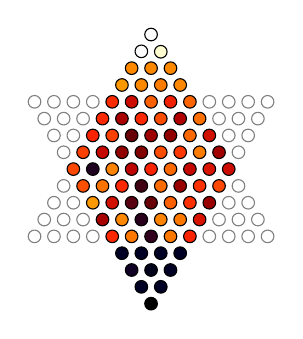
\begin{tikzpicture}
\filldraw [fill=C255] (0.000000,1.708957) circle (0.08); -- 500
\filldraw [fill=C255] (-0.123333,1.495337) circle (0.08); -- 500
\filldraw [fill=C244] (0.123333,1.490204) circle (0.08); -- 476
\filldraw [fill=C106] (-0.246667,1.281718) circle (0.08); -- 200
\filldraw [fill=C106] (0.000000,1.281718) circle (0.08); -- 200
\filldraw [fill=C106] (0.246667,1.281718) circle (0.08); -- 200
\filldraw [fill=C113] (-0.370000,1.068098) circle (0.08); -- 214
\filldraw [fill=C106] (-0.123333,1.068098) circle (0.08); -- 200
\filldraw [fill=C100] (0.123333,1.068098) circle (0.08); -- 188
\filldraw [fill=C106] (0.370000,1.068098) circle (0.08); -- 200
\draw [color=gray] (-1.480000,0.854478) circle (0.08); 
\draw [color=gray] (-1.233333,0.854478) circle (0.08); 
\draw [color=gray] (-0.986667,0.854478) circle (0.08); 
\draw [color=gray] (-0.740000,0.854478) circle (0.08); 
\filldraw [fill=C61] (-0.493333,0.854478) circle (0.08); -- 110
\filldraw [fill=C45] (-0.246667,0.854478) circle (0.08); -- 77
\filldraw [fill=C86] (0.000000,0.854478) circle (0.08); -- 160
\filldraw [fill=C54] (0.246667,0.854478) circle (0.08); -- 95
\filldraw [fill=C88] (0.493333,0.854478) circle (0.08); -- 163
\draw [color=gray] (0.740000,0.854478) circle (0.08); 
\draw [color=gray] (0.986667,0.854478) circle (0.08); 
\draw [color=gray] (1.233333,0.854478) circle (0.08); 
\draw [color=gray] (1.480000,0.854478) circle (0.08); 
\draw [color=gray] (-1.356667,0.640859) circle (0.08); 
\draw [color=gray] (-1.110000,0.640859) circle (0.08); 
\draw [color=gray] (-0.863333,0.640859) circle (0.08); 
\filldraw [fill=C58] (-0.616667,0.640859) circle (0.08); -- 104
\filldraw [fill=C36] (-0.370000,0.640859) circle (0.08); -- 60
\filldraw [fill=C59] (-0.123333,0.640859) circle (0.08); -- 105
\filldraw [fill=C77] (0.123333,0.640859) circle (0.08); -- 141
\filldraw [fill=C38] (0.370000,0.640859) circle (0.08); -- 63
\filldraw [fill=C93] (0.616667,0.640859) circle (0.08); -- 174
\draw [color=gray] (0.863333,0.640859) circle (0.08); 
\draw [color=gray] (1.110000,0.640859) circle (0.08); 
\draw [color=gray] (1.356667,0.640859) circle (0.08); 
\draw [color=gray] (-1.233333,0.427239) circle (0.08); 
\draw [color=gray] (-0.986667,0.427239) circle (0.08); 
\filldraw [fill=C56] (-0.740000,0.427239) circle (0.08); -- 99
\filldraw [fill=C70] (-0.493333,0.427239) circle (0.08); -- 128
\filldraw [fill=C20] (-0.246667,0.427239) circle (0.08); -- 28
\filldraw [fill=C32] (0.000000,0.427239) circle (0.08); -- 52
\filldraw [fill=C29] (0.246667,0.427239) circle (0.08); -- 45
\filldraw [fill=C89] (0.493333,0.427239) circle (0.08); -- 165
\filldraw [fill=C46] (0.740000,0.427239) circle (0.08); -- 79
\draw [color=gray] (0.986667,0.427239) circle (0.08); 
\draw [color=gray] (1.233333,0.427239) circle (0.08); 
\draw [color=gray] (-1.110000,0.213620) circle (0.08); 
\filldraw [fill=C70] (-0.863333,0.213620) circle (0.08); -- 128
\filldraw [fill=C43] (-0.616667,0.213620) circle (0.08); -- 73
\filldraw [fill=C28] (-0.370000,0.213620) circle (0.08); -- 44
\filldraw [fill=C23] (-0.123333,0.213620) circle (0.08); -- 33
\filldraw [fill=C77] (0.123333,0.213620) circle (0.08); -- 142
\filldraw [fill=C66] (0.370000,0.213620) circle (0.08); -- 120
\filldraw [fill=C100] (0.616667,0.213620) circle (0.08); -- 188
\filldraw [fill=C33] (0.863333,0.213620) circle (0.08); -- 54
\draw [color=gray] (1.110000,0.213620) circle (0.08); 
\filldraw [fill=C74] (-0.986667,0.000000) circle (0.08); -- 136
\filldraw [fill=C11] (-0.740000,0.000000) circle (0.08); -- 9
\filldraw [fill=C104] (-0.493333,0.000000) circle (0.08); -- 195
\filldraw [fill=C41] (-0.246667,0.000000) circle (0.08); -- 70
\filldraw [fill=C56] (0.000000,0.000000) circle (0.08); -- 100
\filldraw [fill=C89] (0.246667,0.000000) circle (0.08); -- 166
\filldraw [fill=C43] (0.493333,0.000000) circle (0.08); -- 73
\filldraw [fill=C48] (0.740000,0.000000) circle (0.08); -- 84
\filldraw [fill=C45] (0.986667,0.000000) circle (0.08); -- 77
\draw [color=gray] (-1.110000,-0.213620) circle (0.08); 
\filldraw [fill=C78] (-0.863333,-0.213620) circle (0.08); -- 144
\filldraw [fill=C96] (-0.616667,-0.213620) circle (0.08); -- 179
\filldraw [fill=C59] (-0.370000,-0.213620) circle (0.08); -- 106
\filldraw [fill=C15] (-0.123333,-0.213620) circle (0.08); -- 17
\filldraw [fill=C91] (0.123333,-0.213620) circle (0.08); -- 170
\filldraw [fill=C31] (0.370000,-0.213620) circle (0.08); -- 50
\filldraw [fill=C62] (0.616667,-0.213620) circle (0.08); -- 111
\filldraw [fill=C74] (0.863333,-0.213620) circle (0.08); -- 135
\draw [color=gray] (1.110000,-0.213620) circle (0.08); 
\draw [color=gray] (-1.233333,-0.427239) circle (0.08); 
\draw [color=gray] (-0.986667,-0.427239) circle (0.08); 
\filldraw [fill=C112] (-0.740000,-0.427239) circle (0.08); -- 211
\filldraw [fill=C46] (-0.493333,-0.427239) circle (0.08); -- 80
\filldraw [fill=C18] (-0.246667,-0.427239) circle (0.08); -- 24
\filldraw [fill=C20] (0.000000,-0.427239) circle (0.08); -- 27
\filldraw [fill=C86] (0.246667,-0.427239) circle (0.08); -- 159
\filldraw [fill=C62] (0.493333,-0.427239) circle (0.08); -- 112
\filldraw [fill=C31] (0.740000,-0.427239) circle (0.08); -- 49
\draw [color=gray] (0.986667,-0.427239) circle (0.08); 
\draw [color=gray] (1.233333,-0.427239) circle (0.08); 
\draw [color=gray] (-1.356667,-0.640859) circle (0.08); 
\draw [color=gray] (-1.110000,-0.640859) circle (0.08); 
\draw [color=gray] (-0.863333,-0.640859) circle (0.08); 
\filldraw [fill=C36] (-0.616667,-0.640859) circle (0.08); -- 60
\filldraw [fill=C106] (-0.370000,-0.640859) circle (0.08); -- 199
\filldraw [fill=C12] (-0.123333,-0.640859) circle (0.08); -- 12
\filldraw [fill=C103] (0.123333,-0.640859) circle (0.08); -- 193
\filldraw [fill=C98] (0.370000,-0.640859) circle (0.08); -- 183
\filldraw [fill=C48] (0.616667,-0.640859) circle (0.08); -- 83
\draw [color=gray] (0.863333,-0.640859) circle (0.08); 
\draw [color=gray] (1.110000,-0.640859) circle (0.08); 
\draw [color=gray] (1.356667,-0.640859) circle (0.08); 
\draw [color=gray] (-1.480000,-0.854478) circle (0.08); 
\draw [color=gray] (-1.233333,-0.854478) circle (0.08); 
\draw [color=gray] (-0.986667,-0.854478) circle (0.08); 
\draw [color=gray] (-0.740000,-0.854478) circle (0.08); 
\filldraw [fill=C59] (-0.493333,-0.854478) circle (0.08); -- 106
\filldraw [fill=C97] (-0.246667,-0.854478) circle (0.08); -- 182
\filldraw [fill=C13] (0.000000,-0.854478) circle (0.08); -- 14
\filldraw [fill=C98] (0.246667,-0.854478) circle (0.08); -- 183
\filldraw [fill=C56] (0.493333,-0.854478) circle (0.08); -- 100
\draw [color=gray] (0.740000,-0.854478) circle (0.08); 
\draw [color=gray] (0.986667,-0.854478) circle (0.08); 
\draw [color=gray] (1.233333,-0.854478) circle (0.08); 
\draw [color=gray] (1.480000,-0.854478) circle (0.08); 
\filldraw [fill=C6] (-0.370000,-1.068099) circle (0.08); -- 0
\filldraw [fill=C6] (-0.123333,-1.068099) circle (0.08); -- 0
\filldraw [fill=C6] (0.123333,-1.068099) circle (0.08); -- 0
\filldraw [fill=C6] (0.370000,-1.068099) circle (0.08); -- 0
\filldraw [fill=C9] (-0.246667,-1.281718) circle (0.08); -- 5
\filldraw [fill=C1] (0.000000,-1.281718) circle (0.08); -- -10
\filldraw [fill=C6] (0.246667,-1.281718) circle (0.08); -- 0
\filldraw [fill=C6] (-0.123333,-1.495338) circle (0.08); -- 0
\filldraw [fill=C6] (0.123333,-1.495338) circle (0.08); -- 0
\filldraw [fill=C0] (0.000000,-1.708957) circle (0.08); -- -12
\end{tikzpicture}

\caption{This is the first individual that has actually won a game
  against our hand-tuned bot. It is from generation 51.}
\label{genpop51}
\end{figure}

\begin{figure}
\centering
\definecolor{C0}{rgb}{0.000000,0.000000,0.000000}
\definecolor{C1}{rgb}{0.000000,0.000000,0.094118}
\definecolor{C2}{rgb}{0.000000,0.000000,0.094118}
\definecolor{C3}{rgb}{0.000000,0.000000,0.109804}
\definecolor{C4}{rgb}{0.000000,0.000000,0.125490}
\definecolor{C5}{rgb}{0.000000,0.000000,0.125490}
\definecolor{C6}{rgb}{0.000000,0.000000,0.141176}
\definecolor{C7}{rgb}{0.000000,0.000000,0.156863}
\definecolor{C8}{rgb}{0.031373,0.000000,0.156863}
\definecolor{C9}{rgb}{0.062745,0.000000,0.141176}
\definecolor{C10}{rgb}{0.094118,0.000000,0.141176}
\definecolor{C11}{rgb}{0.125490,0.000000,0.125490}
\definecolor{C12}{rgb}{0.156863,0.000000,0.109804}
\definecolor{C13}{rgb}{0.188235,0.000000,0.109804}
\definecolor{C14}{rgb}{0.219608,0.000000,0.094118}
\definecolor{C15}{rgb}{0.250980,0.000000,0.078431}
\definecolor{C16}{rgb}{0.282353,0.000000,0.078431}
\definecolor{C17}{rgb}{0.313725,0.000000,0.062745}
\definecolor{C18}{rgb}{0.345098,0.000000,0.062745}
\definecolor{C19}{rgb}{0.376471,0.000000,0.047059}
\definecolor{C20}{rgb}{0.407843,0.000000,0.031373}
\definecolor{C21}{rgb}{0.439216,0.000000,0.031373}
\definecolor{C22}{rgb}{0.470588,0.000000,0.015686}
\definecolor{C23}{rgb}{0.501961,0.000000,0.000000}
\definecolor{C24}{rgb}{0.501961,0.000000,0.000000}
\definecolor{C25}{rgb}{0.517647,0.000000,0.000000}
\definecolor{C26}{rgb}{0.533333,0.000000,0.000000}
\definecolor{C27}{rgb}{0.549020,0.000000,0.000000}
\definecolor{C28}{rgb}{0.564706,0.000000,0.000000}
\definecolor{C29}{rgb}{0.564706,0.000000,0.000000}
\definecolor{C30}{rgb}{0.580392,0.000000,0.000000}
\definecolor{C31}{rgb}{0.596078,0.000000,0.000000}
\definecolor{C32}{rgb}{0.611765,0.000000,0.000000}
\definecolor{C33}{rgb}{0.627451,0.000000,0.000000}
\definecolor{C34}{rgb}{0.627451,0.000000,0.000000}
\definecolor{C35}{rgb}{0.643137,0.000000,0.000000}
\definecolor{C36}{rgb}{0.658824,0.000000,0.000000}
\definecolor{C37}{rgb}{0.674510,0.000000,0.000000}
\definecolor{C38}{rgb}{0.690196,0.000000,0.000000}
\definecolor{C39}{rgb}{0.705882,0.000000,0.000000}
\definecolor{C40}{rgb}{0.721569,0.015686,0.000000}
\definecolor{C41}{rgb}{0.737255,0.015686,0.000000}
\definecolor{C42}{rgb}{0.752941,0.031373,0.000000}
\definecolor{C43}{rgb}{0.768627,0.031373,0.000000}
\definecolor{C44}{rgb}{0.784314,0.047059,0.000000}
\definecolor{C45}{rgb}{0.800000,0.047059,0.000000}
\definecolor{C46}{rgb}{0.815686,0.062745,0.000000}
\definecolor{C47}{rgb}{0.831373,0.062745,0.000000}
\definecolor{C48}{rgb}{0.847059,0.078431,0.000000}
\definecolor{C49}{rgb}{0.862745,0.078431,0.000000}
\definecolor{C50}{rgb}{0.878431,0.094118,0.000000}
\definecolor{C51}{rgb}{0.894118,0.094118,0.000000}
\definecolor{C52}{rgb}{0.909804,0.109804,0.000000}
\definecolor{C53}{rgb}{0.925490,0.109804,0.000000}
\definecolor{C54}{rgb}{0.941176,0.125490,0.000000}
\definecolor{C55}{rgb}{0.956863,0.125490,0.000000}
\definecolor{C56}{rgb}{0.988235,0.141176,0.000000}
\definecolor{C57}{rgb}{0.988235,0.141176,0.000000}
\definecolor{C58}{rgb}{0.988235,0.156863,0.000000}
\definecolor{C59}{rgb}{0.988235,0.156863,0.000000}
\definecolor{C60}{rgb}{0.988235,0.172549,0.000000}
\definecolor{C61}{rgb}{0.988235,0.172549,0.000000}
\definecolor{C62}{rgb}{0.988235,0.188235,0.000000}
\definecolor{C63}{rgb}{0.988235,0.188235,0.000000}
\definecolor{C64}{rgb}{0.988235,0.203922,0.000000}
\definecolor{C65}{rgb}{0.988235,0.203922,0.000000}
\definecolor{C66}{rgb}{0.988235,0.219608,0.000000}
\definecolor{C67}{rgb}{0.988235,0.219608,0.000000}
\definecolor{C68}{rgb}{0.988235,0.235294,0.000000}
\definecolor{C69}{rgb}{0.988235,0.235294,0.000000}
\definecolor{C70}{rgb}{0.988235,0.250980,0.000000}
\definecolor{C71}{rgb}{0.988235,0.250980,0.000000}
\definecolor{C72}{rgb}{0.988235,0.266667,0.000000}
\definecolor{C73}{rgb}{0.988235,0.266667,0.000000}
\definecolor{C74}{rgb}{0.988235,0.282353,0.000000}
\definecolor{C75}{rgb}{0.988235,0.282353,0.000000}
\definecolor{C76}{rgb}{0.988235,0.298039,0.000000}
\definecolor{C77}{rgb}{0.988235,0.298039,0.000000}
\definecolor{C78}{rgb}{0.988235,0.313725,0.000000}
\definecolor{C79}{rgb}{0.988235,0.313725,0.000000}
\definecolor{C80}{rgb}{0.988235,0.329412,0.000000}
\definecolor{C81}{rgb}{0.988235,0.329412,0.000000}
\definecolor{C82}{rgb}{0.988235,0.345098,0.000000}
\definecolor{C83}{rgb}{0.988235,0.345098,0.000000}
\definecolor{C84}{rgb}{0.988235,0.360784,0.000000}
\definecolor{C85}{rgb}{0.988235,0.376471,0.000000}
\definecolor{C86}{rgb}{0.988235,0.376471,0.000000}
\definecolor{C87}{rgb}{0.988235,0.392157,0.000000}
\definecolor{C88}{rgb}{0.988235,0.392157,0.000000}
\definecolor{C89}{rgb}{0.988235,0.407843,0.000000}
\definecolor{C90}{rgb}{0.988235,0.407843,0.000000}
\definecolor{C91}{rgb}{0.988235,0.423529,0.000000}
\definecolor{C92}{rgb}{0.988235,0.423529,0.000000}
\definecolor{C93}{rgb}{0.988235,0.439216,0.000000}
\definecolor{C94}{rgb}{0.988235,0.439216,0.000000}
\definecolor{C95}{rgb}{0.988235,0.454902,0.000000}
\definecolor{C96}{rgb}{0.988235,0.454902,0.000000}
\definecolor{C97}{rgb}{0.988235,0.470588,0.000000}
\definecolor{C98}{rgb}{0.988235,0.470588,0.000000}
\definecolor{C99}{rgb}{0.988235,0.486275,0.000000}
\definecolor{C100}{rgb}{0.988235,0.486275,0.000000}
\definecolor{C101}{rgb}{0.988235,0.501961,0.000000}
\definecolor{C102}{rgb}{0.988235,0.501961,0.000000}
\definecolor{C103}{rgb}{0.988235,0.517647,0.000000}
\definecolor{C104}{rgb}{0.988235,0.517647,0.000000}
\definecolor{C105}{rgb}{0.988235,0.533333,0.000000}
\definecolor{C106}{rgb}{0.988235,0.533333,0.000000}
\definecolor{C107}{rgb}{0.988235,0.549020,0.000000}
\definecolor{C108}{rgb}{0.988235,0.549020,0.000000}
\definecolor{C109}{rgb}{0.988235,0.564706,0.000000}
\definecolor{C110}{rgb}{0.988235,0.564706,0.000000}
\definecolor{C111}{rgb}{0.988235,0.580392,0.000000}
\definecolor{C112}{rgb}{0.988235,0.596078,0.000000}
\definecolor{C113}{rgb}{0.988235,0.596078,0.000000}
\definecolor{C114}{rgb}{0.988235,0.611765,0.000000}
\definecolor{C115}{rgb}{0.988235,0.611765,0.000000}
\definecolor{C116}{rgb}{0.988235,0.627451,0.000000}
\definecolor{C117}{rgb}{0.988235,0.627451,0.000000}
\definecolor{C118}{rgb}{0.988235,0.643137,0.000000}
\definecolor{C119}{rgb}{0.988235,0.643137,0.000000}
\definecolor{C120}{rgb}{0.988235,0.658824,0.000000}
\definecolor{C121}{rgb}{0.988235,0.658824,0.000000}
\definecolor{C122}{rgb}{0.988235,0.674510,0.000000}
\definecolor{C123}{rgb}{0.988235,0.674510,0.000000}
\definecolor{C124}{rgb}{0.988235,0.690196,0.000000}
\definecolor{C125}{rgb}{0.988235,0.690196,0.000000}
\definecolor{C126}{rgb}{0.988235,0.705882,0.000000}
\definecolor{C127}{rgb}{0.988235,0.705882,0.000000}
\definecolor{C128}{rgb}{0.988235,0.721569,0.000000}
\definecolor{C129}{rgb}{0.988235,0.721569,0.000000}
\definecolor{C130}{rgb}{0.988235,0.737255,0.000000}
\definecolor{C131}{rgb}{0.988235,0.737255,0.000000}
\definecolor{C132}{rgb}{0.988235,0.752941,0.000000}
\definecolor{C133}{rgb}{0.988235,0.752941,0.000000}
\definecolor{C134}{rgb}{0.988235,0.768627,0.000000}
\definecolor{C135}{rgb}{0.988235,0.768627,0.000000}
\definecolor{C136}{rgb}{0.988235,0.784314,0.000000}
\definecolor{C137}{rgb}{0.988235,0.784314,0.000000}
\definecolor{C138}{rgb}{0.988235,0.800000,0.000000}
\definecolor{C139}{rgb}{0.988235,0.815686,0.000000}
\definecolor{C140}{rgb}{0.988235,0.815686,0.000000}
\definecolor{C141}{rgb}{0.988235,0.815686,0.000000}
\definecolor{C142}{rgb}{0.988235,0.815686,0.000000}
\definecolor{C143}{rgb}{0.988235,0.815686,0.000000}
\definecolor{C144}{rgb}{0.988235,0.831373,0.000000}
\definecolor{C145}{rgb}{0.988235,0.831373,0.000000}
\definecolor{C146}{rgb}{0.988235,0.831373,0.000000}
\definecolor{C147}{rgb}{0.988235,0.831373,0.000000}
\definecolor{C148}{rgb}{0.988235,0.847059,0.000000}
\definecolor{C149}{rgb}{0.988235,0.847059,0.000000}
\definecolor{C150}{rgb}{0.988235,0.847059,0.000000}
\definecolor{C151}{rgb}{0.988235,0.847059,0.000000}
\definecolor{C152}{rgb}{0.988235,0.847059,0.000000}
\definecolor{C153}{rgb}{0.988235,0.862745,0.000000}
\definecolor{C154}{rgb}{0.988235,0.862745,0.000000}
\definecolor{C155}{rgb}{0.988235,0.862745,0.000000}
\definecolor{C156}{rgb}{0.988235,0.862745,0.000000}
\definecolor{C157}{rgb}{0.988235,0.878431,0.000000}
\definecolor{C158}{rgb}{0.988235,0.878431,0.000000}
\definecolor{C159}{rgb}{0.988235,0.878431,0.000000}
\definecolor{C160}{rgb}{0.988235,0.878431,0.000000}
\definecolor{C161}{rgb}{0.988235,0.894118,0.000000}
\definecolor{C162}{rgb}{0.988235,0.894118,0.000000}
\definecolor{C163}{rgb}{0.988235,0.894118,0.000000}
\definecolor{C164}{rgb}{0.988235,0.894118,0.000000}
\definecolor{C165}{rgb}{0.988235,0.894118,0.000000}
\definecolor{C166}{rgb}{0.988235,0.909804,0.000000}
\definecolor{C167}{rgb}{0.988235,0.909804,0.000000}
\definecolor{C168}{rgb}{0.988235,0.909804,0.000000}
\definecolor{C169}{rgb}{0.988235,0.909804,0.000000}
\definecolor{C170}{rgb}{0.988235,0.925490,0.000000}
\definecolor{C171}{rgb}{0.988235,0.925490,0.000000}
\definecolor{C172}{rgb}{0.988235,0.925490,0.000000}
\definecolor{C173}{rgb}{0.988235,0.925490,0.000000}
\definecolor{C174}{rgb}{0.988235,0.941176,0.000000}
\definecolor{C175}{rgb}{0.988235,0.941176,0.000000}
\definecolor{C176}{rgb}{0.988235,0.941176,0.000000}
\definecolor{C177}{rgb}{0.988235,0.941176,0.000000}
\definecolor{C178}{rgb}{0.988235,0.941176,0.000000}
\definecolor{C179}{rgb}{0.988235,0.956863,0.000000}
\definecolor{C180}{rgb}{0.988235,0.956863,0.000000}
\definecolor{C181}{rgb}{0.988235,0.956863,0.000000}
\definecolor{C182}{rgb}{0.988235,0.956863,0.000000}
\definecolor{C183}{rgb}{0.988235,0.972549,0.000000}
\definecolor{C184}{rgb}{0.988235,0.972549,0.000000}
\definecolor{C185}{rgb}{0.988235,0.972549,0.000000}
\definecolor{C186}{rgb}{0.988235,0.972549,0.000000}
\definecolor{C187}{rgb}{0.988235,0.988235,0.000000}
\definecolor{C188}{rgb}{0.988235,0.988235,0.015686}
\definecolor{C189}{rgb}{0.988235,0.988235,0.031373}
\definecolor{C190}{rgb}{0.988235,0.988235,0.047059}
\definecolor{C191}{rgb}{0.988235,0.988235,0.062745}
\definecolor{C192}{rgb}{0.988235,0.988235,0.078431}
\definecolor{C193}{rgb}{0.988235,0.988235,0.094118}
\definecolor{C194}{rgb}{0.988235,0.988235,0.109804}
\definecolor{C195}{rgb}{0.988235,0.988235,0.125490}
\definecolor{C196}{rgb}{0.988235,0.988235,0.141176}
\definecolor{C197}{rgb}{0.988235,0.988235,0.156863}
\definecolor{C198}{rgb}{0.988235,0.988235,0.156863}
\definecolor{C199}{rgb}{0.988235,0.988235,0.172549}
\definecolor{C200}{rgb}{0.988235,0.988235,0.188235}
\definecolor{C201}{rgb}{0.988235,0.988235,0.203922}
\definecolor{C202}{rgb}{0.988235,0.988235,0.219608}
\definecolor{C203}{rgb}{0.988235,0.988235,0.235294}
\definecolor{C204}{rgb}{0.988235,0.988235,0.250980}
\definecolor{C205}{rgb}{0.988235,0.988235,0.266667}
\definecolor{C206}{rgb}{0.988235,0.988235,0.282353}
\definecolor{C207}{rgb}{0.988235,0.988235,0.298039}
\definecolor{C208}{rgb}{0.988235,0.988235,0.313725}
\definecolor{C209}{rgb}{0.988235,0.988235,0.329412}
\definecolor{C210}{rgb}{0.988235,0.988235,0.329412}
\definecolor{C211}{rgb}{0.988235,0.988235,0.345098}
\definecolor{C212}{rgb}{0.988235,0.988235,0.360784}
\definecolor{C213}{rgb}{0.988235,0.988235,0.376471}
\definecolor{C214}{rgb}{0.988235,0.988235,0.392157}
\definecolor{C215}{rgb}{0.988235,0.988235,0.407843}
\definecolor{C216}{rgb}{0.988235,0.988235,0.423529}
\definecolor{C217}{rgb}{0.988235,0.988235,0.439216}
\definecolor{C218}{rgb}{0.988235,0.988235,0.454902}
\definecolor{C219}{rgb}{0.988235,0.988235,0.470588}
\definecolor{C220}{rgb}{0.988235,0.988235,0.486275}
\definecolor{C221}{rgb}{0.988235,0.988235,0.486275}
\definecolor{C222}{rgb}{0.988235,0.988235,0.501961}
\definecolor{C223}{rgb}{0.988235,0.988235,0.517647}
\definecolor{C224}{rgb}{0.988235,0.988235,0.533333}
\definecolor{C225}{rgb}{0.988235,0.988235,0.549020}
\definecolor{C226}{rgb}{0.988235,0.988235,0.564706}
\definecolor{C227}{rgb}{0.988235,0.988235,0.580392}
\definecolor{C228}{rgb}{0.988235,0.988235,0.596078}
\definecolor{C229}{rgb}{0.988235,0.988235,0.611765}
\definecolor{C230}{rgb}{0.988235,0.988235,0.627451}
\definecolor{C231}{rgb}{0.988235,0.988235,0.643137}
\definecolor{C232}{rgb}{0.988235,0.988235,0.658824}
\definecolor{C233}{rgb}{0.988235,0.988235,0.658824}
\definecolor{C234}{rgb}{0.988235,0.988235,0.674510}
\definecolor{C235}{rgb}{0.988235,0.988235,0.690196}
\definecolor{C236}{rgb}{0.988235,0.988235,0.705882}
\definecolor{C237}{rgb}{0.988235,0.988235,0.721569}
\definecolor{C238}{rgb}{0.988235,0.988235,0.737255}
\definecolor{C239}{rgb}{0.988235,0.988235,0.752941}
\definecolor{C240}{rgb}{0.988235,0.988235,0.768627}
\definecolor{C241}{rgb}{0.988235,0.988235,0.784314}
\definecolor{C242}{rgb}{0.988235,0.988235,0.800000}
\definecolor{C243}{rgb}{0.988235,0.988235,0.815686}
\definecolor{C244}{rgb}{0.988235,0.988235,0.815686}
\definecolor{C245}{rgb}{0.988235,0.988235,0.831373}
\definecolor{C246}{rgb}{0.988235,0.988235,0.847059}
\definecolor{C247}{rgb}{0.988235,0.988235,0.862745}
\definecolor{C248}{rgb}{0.988235,0.988235,0.878431}
\definecolor{C249}{rgb}{0.988235,0.988235,0.894118}
\definecolor{C250}{rgb}{0.988235,0.988235,0.909804}
\definecolor{C251}{rgb}{0.988235,0.988235,0.925490}
\definecolor{C252}{rgb}{0.988235,0.988235,0.941176}
\definecolor{C253}{rgb}{0.988235,0.988235,0.956863}
\definecolor{C254}{rgb}{0.988235,0.988235,0.972549}
\definecolor{C255}{rgb}{0.988235,0.988235,0.988235}

%% vec = (46, 172, 25, 127, 500, 133, 123, 170, 128, 188, 145, 152, 56, 136, 7, 86, 56, 111, 98, 33, 183, 479, 437, 40, 148, 79, 145, 104, 160, 46, 174, 89, 126, 10, 48, 36, 11, 146, 217, 207, 184, 28, 93, 94, 78, 29, 84, 39, 39, 69, 135, 188, 17, 131, 107, 213, 182, 164, 215, 99, 174, 39, 19, 109, 96, 41, 173, 157, 234, 172, 70, 131, 107, 96, 163, 115, 142, 28, 19, 16, 9, 161, 139, 30, 79, 41, 154, 75, 148, 132, 60, 93, 129, 74, 207, 103, 141, 42, 40, 184, 145, 59, 87, 5, 185, 153, 65, 113, 53, 52, 58, 153, 79, 51, 180, 6, 101, 35, 67, 8, 138, 190, 166, 89, 69, 45, 33, 138, 96, 191, 49, 96, 211, 132, 23, 180, 171, 104, 92, 200, 157, 53, 233, 27, 49, 139, 106, 105, 77, 24, 77, 176, 118, 29, 29, 193, 158, 128, 185, 144, 126, 23, 186, 78, 98, 216, 188, 98, 133, 127, 183, 112, 17, 83, 233, 27, 184, 84, 24, 22, 117, 123, 49, 60, 38, 187, 99, 100, 45, 52, 144, 154, 191, 123, 73, 187, 21, 182, 214, 105, 134, 93, 47, 36, 22, 200, 61, 105, 165, 97, 179, 148, 112, 166, 5, 141, 79, 202, 7, 87, 183, 128, 146, 83, 75, 52, 123, 134, 55, 52, -34, 3, 5, 0, 97, 229, 45, 144, 166, 19, 38, 38, 163, 29, 35, 47, 154, 177, 5, -10, -3, 40, 24, 162, 27, 197, 4, 8, 118, 8, 197, 214, 125, 62, 106, 95, 0, 0, 20, 102, 80, 22, 198, 48, 128, 83, 142, 133, 61, 6, 163, 44, 10, 168, -27, 177, 174, 213, 177)
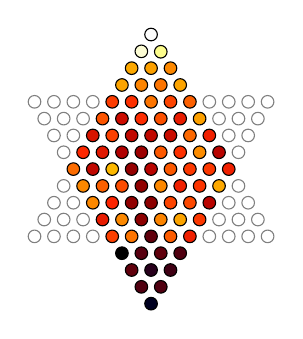
\begin{tikzpicture}
\filldraw [fill=C255] (0.000000,1.708957) circle (0.08); -- 500
\filldraw [fill=C245] (-0.123333,1.495337) circle (0.08); -- 479
\filldraw [fill=C225] (0.123333,1.490204) circle (0.08); -- 437
\filldraw [fill=C120] (-0.246667,1.281718) circle (0.08); -- 217
\filldraw [fill=C116] (0.000000,1.281718) circle (0.08); -- 207
\filldraw [fill=C105] (0.246667,1.281718) circle (0.08); -- 184
\filldraw [fill=C118] (-0.370000,1.068098) circle (0.08); -- 213
\filldraw [fill=C104] (-0.123333,1.068098) circle (0.08); -- 182
\filldraw [fill=C95] (0.123333,1.068098) circle (0.08); -- 164
\filldraw [fill=C119] (0.370000,1.068098) circle (0.08); -- 215
\draw [color=gray] (-1.480000,0.854478) circle (0.08); 
\draw [color=gray] (-1.233333,0.854478) circle (0.08); 
\draw [color=gray] (-0.986667,0.854478) circle (0.08); 
\draw [color=gray] (-0.740000,0.854478) circle (0.08); 
\filldraw [fill=C68] (-0.493333,0.854478) circle (0.08); -- 107
\filldraw [fill=C63] (-0.246667,0.854478) circle (0.08); -- 96
\filldraw [fill=C95] (0.000000,0.854478) circle (0.08); -- 163
\filldraw [fill=C72] (0.246667,0.854478) circle (0.08); -- 115
\filldraw [fill=C85] (0.493333,0.854478) circle (0.08); -- 142
\draw [color=gray] (0.740000,0.854478) circle (0.08); 
\draw [color=gray] (0.986667,0.854478) circle (0.08); 
\draw [color=gray] (1.233333,0.854478) circle (0.08); 
\draw [color=gray] (1.480000,0.854478) circle (0.08); 
\draw [color=gray] (-1.356667,0.640859) circle (0.08); 
\draw [color=gray] (-1.110000,0.640859) circle (0.08); 
\draw [color=gray] (-0.863333,0.640859) circle (0.08); 
\filldraw [fill=C80] (-0.616667,0.640859) circle (0.08); -- 132
\filldraw [fill=C45] (-0.370000,0.640859) circle (0.08); -- 60
\filldraw [fill=C61] (-0.123333,0.640859) circle (0.08); -- 93
\filldraw [fill=C78] (0.123333,0.640859) circle (0.08); -- 129
\filldraw [fill=C52] (0.370000,0.640859) circle (0.08); -- 74
\filldraw [fill=C116] (0.616667,0.640859) circle (0.08); -- 207
\draw [color=gray] (0.863333,0.640859) circle (0.08); 
\draw [color=gray] (1.110000,0.640859) circle (0.08); 
\draw [color=gray] (1.356667,0.640859) circle (0.08); 
\draw [color=gray] (-1.233333,0.427239) circle (0.08); 
\draw [color=gray] (-0.986667,0.427239) circle (0.08); 
\filldraw [fill=C48] (-0.740000,0.427239) circle (0.08); -- 65
\filldraw [fill=C71] (-0.493333,0.427239) circle (0.08); -- 113
\filldraw [fill=C42] (-0.246667,0.427239) circle (0.08); -- 53
\filldraw [fill=C42] (0.000000,0.427239) circle (0.08); -- 52
\filldraw [fill=C44] (0.246667,0.427239) circle (0.08); -- 58
\filldraw [fill=C90] (0.493333,0.427239) circle (0.08); -- 153
\filldraw [fill=C54] (0.740000,0.427239) circle (0.08); -- 79
\draw [color=gray] (0.986667,0.427239) circle (0.08); 
\draw [color=gray] (1.233333,0.427239) circle (0.08); 
\draw [color=gray] (-1.110000,0.213620) circle (0.08); 
\filldraw [fill=C59] (-0.863333,0.213620) circle (0.08); -- 89
\filldraw [fill=C50] (-0.616667,0.213620) circle (0.08); -- 69
\filldraw [fill=C38] (-0.370000,0.213620) circle (0.08); -- 45
\filldraw [fill=C32] (-0.123333,0.213620) circle (0.08); -- 33
\filldraw [fill=C83] (0.123333,0.213620) circle (0.08); -- 138
\filldraw [fill=C63] (0.370000,0.213620) circle (0.08); -- 96
\filldraw [fill=C108] (0.616667,0.213620) circle (0.08); -- 191
\filldraw [fill=C40] (0.863333,0.213620) circle (0.08); -- 49
\draw [color=gray] (1.110000,0.213620) circle (0.08); 
\filldraw [fill=C92] (-0.986667,0.000000) circle (0.08); -- 157
\filldraw [fill=C42] (-0.740000,0.000000) circle (0.08); -- 53
\filldraw [fill=C128] (-0.493333,0.000000) circle (0.08); -- 233
\filldraw [fill=C30] (-0.246667,0.000000) circle (0.08); -- 27
\filldraw [fill=C40] (0.000000,0.000000) circle (0.08); -- 49
\filldraw [fill=C83] (0.246667,0.000000) circle (0.08); -- 139
\filldraw [fill=C67] (0.493333,0.000000) circle (0.08); -- 106
\filldraw [fill=C67] (0.740000,0.000000) circle (0.08); -- 105
\filldraw [fill=C54] (0.986667,0.000000) circle (0.08); -- 77
\draw [color=gray] (-1.110000,-0.213620) circle (0.08); 
\filldraw [fill=C105] (-0.863333,-0.213620) circle (0.08); -- 185
\filldraw [fill=C85] (-0.616667,-0.213620) circle (0.08); -- 144
\filldraw [fill=C77] (-0.370000,-0.213620) circle (0.08); -- 126
\filldraw [fill=C28] (-0.123333,-0.213620) circle (0.08); -- 23
\filldraw [fill=C106] (0.123333,-0.213620) circle (0.08); -- 186
\filldraw [fill=C54] (0.370000,-0.213620) circle (0.08); -- 78
\filldraw [fill=C64] (0.616667,-0.213620) circle (0.08); -- 98
\filldraw [fill=C120] (0.863333,-0.213620) circle (0.08); -- 216
\draw [color=gray] (1.110000,-0.213620) circle (0.08); 
\draw [color=gray] (-1.233333,-0.427239) circle (0.08); 
\draw [color=gray] (-0.986667,-0.427239) circle (0.08); 
\filldraw [fill=C105] (-0.740000,-0.427239) circle (0.08); -- 184
\filldraw [fill=C57] (-0.493333,-0.427239) circle (0.08); -- 84
\filldraw [fill=C28] (-0.246667,-0.427239) circle (0.08); -- 24
\filldraw [fill=C27] (0.000000,-0.427239) circle (0.08); -- 22
\filldraw [fill=C73] (0.246667,-0.427239) circle (0.08); -- 117
\filldraw [fill=C75] (0.493333,-0.427239) circle (0.08); -- 123
\filldraw [fill=C40] (0.740000,-0.427239) circle (0.08); -- 49
\draw [color=gray] (0.986667,-0.427239) circle (0.08); 
\draw [color=gray] (1.233333,-0.427239) circle (0.08); 
\draw [color=gray] (-1.356667,-0.640859) circle (0.08); 
\draw [color=gray] (-1.110000,-0.640859) circle (0.08); 
\draw [color=gray] (-0.863333,-0.640859) circle (0.08); 
\filldraw [fill=C52] (-0.616667,-0.640859) circle (0.08); -- 73
\filldraw [fill=C106] (-0.370000,-0.640859) circle (0.08); -- 187
\filldraw [fill=C27] (-0.123333,-0.640859) circle (0.08); -- 21
\filldraw [fill=C104] (0.123333,-0.640859) circle (0.08); -- 182
\filldraw [fill=C119] (0.370000,-0.640859) circle (0.08); -- 214
\filldraw [fill=C67] (0.616667,-0.640859) circle (0.08); -- 105
\draw [color=gray] (0.863333,-0.640859) circle (0.08); 
\draw [color=gray] (1.110000,-0.640859) circle (0.08); 
\draw [color=gray] (1.356667,-0.640859) circle (0.08); 
\draw [color=gray] (-1.480000,-0.854478) circle (0.08); 
\draw [color=gray] (-1.233333,-0.854478) circle (0.08); 
\draw [color=gray] (-0.986667,-0.854478) circle (0.08); 
\draw [color=gray] (-0.740000,-0.854478) circle (0.08); 
\filldraw [fill=C70] (-0.493333,-0.854478) circle (0.08); -- 112
\filldraw [fill=C96] (-0.246667,-0.854478) circle (0.08); -- 166
\filldraw [fill=C19] (0.000000,-0.854478) circle (0.08); -- 5
\filldraw [fill=C84] (0.246667,-0.854478) circle (0.08); -- 141
\filldraw [fill=C54] (0.493333,-0.854478) circle (0.08); -- 79
\draw [color=gray] (0.740000,-0.854478) circle (0.08); 
\draw [color=gray] (0.986667,-0.854478) circle (0.08); 
\draw [color=gray] (1.233333,-0.854478) circle (0.08); 
\draw [color=gray] (1.480000,-0.854478) circle (0.08); 
\filldraw [fill=C0] (-0.370000,-1.068099) circle (0.08); -- -34
\filldraw [fill=C18] (-0.123333,-1.068099) circle (0.08); -- 3
\filldraw [fill=C19] (0.123333,-1.068099) circle (0.08); -- 5
\filldraw [fill=C17] (0.370000,-1.068099) circle (0.08); -- 0
\filldraw [fill=C19] (-0.246667,-1.281718) circle (0.08); -- 5
\filldraw [fill=C12] (0.000000,-1.281718) circle (0.08); -- -10
\filldraw [fill=C15] (0.246667,-1.281718) circle (0.08); -- -3
\filldraw [fill=C17] (-0.123333,-1.495338) circle (0.08); -- 0
\filldraw [fill=C17] (0.123333,-1.495338) circle (0.08); -- 0
\filldraw [fill=C4] (0.000000,-1.708957) circle (0.08); -- -27
\end{tikzpicture}

\caption{The individuals from generation 2427 won every game they
  played when the genetic algorithm was running. Each individual is
  only tested five times by the algorithm, but more extensive
  experiments show that this individual wins around $99\%$ of the
  games it plays. The fitness of this individual was $416.6$.}
\label{genpop2427}
\end{figure}

\begin{figure}
\centering
\definecolor{C0}{rgb}{0.000000,0.000000,0.000000}
\definecolor{C1}{rgb}{0.000000,0.000000,0.094118}
\definecolor{C2}{rgb}{0.000000,0.000000,0.094118}
\definecolor{C3}{rgb}{0.000000,0.000000,0.109804}
\definecolor{C4}{rgb}{0.000000,0.000000,0.125490}
\definecolor{C5}{rgb}{0.000000,0.000000,0.125490}
\definecolor{C6}{rgb}{0.000000,0.000000,0.141176}
\definecolor{C7}{rgb}{0.000000,0.000000,0.156863}
\definecolor{C8}{rgb}{0.031373,0.000000,0.156863}
\definecolor{C9}{rgb}{0.062745,0.000000,0.141176}
\definecolor{C10}{rgb}{0.094118,0.000000,0.141176}
\definecolor{C11}{rgb}{0.125490,0.000000,0.125490}
\definecolor{C12}{rgb}{0.156863,0.000000,0.109804}
\definecolor{C13}{rgb}{0.188235,0.000000,0.109804}
\definecolor{C14}{rgb}{0.219608,0.000000,0.094118}
\definecolor{C15}{rgb}{0.250980,0.000000,0.078431}
\definecolor{C16}{rgb}{0.282353,0.000000,0.078431}
\definecolor{C17}{rgb}{0.313725,0.000000,0.062745}
\definecolor{C18}{rgb}{0.345098,0.000000,0.062745}
\definecolor{C19}{rgb}{0.376471,0.000000,0.047059}
\definecolor{C20}{rgb}{0.407843,0.000000,0.031373}
\definecolor{C21}{rgb}{0.439216,0.000000,0.031373}
\definecolor{C22}{rgb}{0.470588,0.000000,0.015686}
\definecolor{C23}{rgb}{0.501961,0.000000,0.000000}
\definecolor{C24}{rgb}{0.501961,0.000000,0.000000}
\definecolor{C25}{rgb}{0.517647,0.000000,0.000000}
\definecolor{C26}{rgb}{0.533333,0.000000,0.000000}
\definecolor{C27}{rgb}{0.549020,0.000000,0.000000}
\definecolor{C28}{rgb}{0.564706,0.000000,0.000000}
\definecolor{C29}{rgb}{0.564706,0.000000,0.000000}
\definecolor{C30}{rgb}{0.580392,0.000000,0.000000}
\definecolor{C31}{rgb}{0.596078,0.000000,0.000000}
\definecolor{C32}{rgb}{0.611765,0.000000,0.000000}
\definecolor{C33}{rgb}{0.627451,0.000000,0.000000}
\definecolor{C34}{rgb}{0.627451,0.000000,0.000000}
\definecolor{C35}{rgb}{0.643137,0.000000,0.000000}
\definecolor{C36}{rgb}{0.658824,0.000000,0.000000}
\definecolor{C37}{rgb}{0.674510,0.000000,0.000000}
\definecolor{C38}{rgb}{0.690196,0.000000,0.000000}
\definecolor{C39}{rgb}{0.705882,0.000000,0.000000}
\definecolor{C40}{rgb}{0.721569,0.015686,0.000000}
\definecolor{C41}{rgb}{0.737255,0.015686,0.000000}
\definecolor{C42}{rgb}{0.752941,0.031373,0.000000}
\definecolor{C43}{rgb}{0.768627,0.031373,0.000000}
\definecolor{C44}{rgb}{0.784314,0.047059,0.000000}
\definecolor{C45}{rgb}{0.800000,0.047059,0.000000}
\definecolor{C46}{rgb}{0.815686,0.062745,0.000000}
\definecolor{C47}{rgb}{0.831373,0.062745,0.000000}
\definecolor{C48}{rgb}{0.847059,0.078431,0.000000}
\definecolor{C49}{rgb}{0.862745,0.078431,0.000000}
\definecolor{C50}{rgb}{0.878431,0.094118,0.000000}
\definecolor{C51}{rgb}{0.894118,0.094118,0.000000}
\definecolor{C52}{rgb}{0.909804,0.109804,0.000000}
\definecolor{C53}{rgb}{0.925490,0.109804,0.000000}
\definecolor{C54}{rgb}{0.941176,0.125490,0.000000}
\definecolor{C55}{rgb}{0.956863,0.125490,0.000000}
\definecolor{C56}{rgb}{0.988235,0.141176,0.000000}
\definecolor{C57}{rgb}{0.988235,0.141176,0.000000}
\definecolor{C58}{rgb}{0.988235,0.156863,0.000000}
\definecolor{C59}{rgb}{0.988235,0.156863,0.000000}
\definecolor{C60}{rgb}{0.988235,0.172549,0.000000}
\definecolor{C61}{rgb}{0.988235,0.172549,0.000000}
\definecolor{C62}{rgb}{0.988235,0.188235,0.000000}
\definecolor{C63}{rgb}{0.988235,0.188235,0.000000}
\definecolor{C64}{rgb}{0.988235,0.203922,0.000000}
\definecolor{C65}{rgb}{0.988235,0.203922,0.000000}
\definecolor{C66}{rgb}{0.988235,0.219608,0.000000}
\definecolor{C67}{rgb}{0.988235,0.219608,0.000000}
\definecolor{C68}{rgb}{0.988235,0.235294,0.000000}
\definecolor{C69}{rgb}{0.988235,0.235294,0.000000}
\definecolor{C70}{rgb}{0.988235,0.250980,0.000000}
\definecolor{C71}{rgb}{0.988235,0.250980,0.000000}
\definecolor{C72}{rgb}{0.988235,0.266667,0.000000}
\definecolor{C73}{rgb}{0.988235,0.266667,0.000000}
\definecolor{C74}{rgb}{0.988235,0.282353,0.000000}
\definecolor{C75}{rgb}{0.988235,0.282353,0.000000}
\definecolor{C76}{rgb}{0.988235,0.298039,0.000000}
\definecolor{C77}{rgb}{0.988235,0.298039,0.000000}
\definecolor{C78}{rgb}{0.988235,0.313725,0.000000}
\definecolor{C79}{rgb}{0.988235,0.313725,0.000000}
\definecolor{C80}{rgb}{0.988235,0.329412,0.000000}
\definecolor{C81}{rgb}{0.988235,0.329412,0.000000}
\definecolor{C82}{rgb}{0.988235,0.345098,0.000000}
\definecolor{C83}{rgb}{0.988235,0.345098,0.000000}
\definecolor{C84}{rgb}{0.988235,0.360784,0.000000}
\definecolor{C85}{rgb}{0.988235,0.376471,0.000000}
\definecolor{C86}{rgb}{0.988235,0.376471,0.000000}
\definecolor{C87}{rgb}{0.988235,0.392157,0.000000}
\definecolor{C88}{rgb}{0.988235,0.392157,0.000000}
\definecolor{C89}{rgb}{0.988235,0.407843,0.000000}
\definecolor{C90}{rgb}{0.988235,0.407843,0.000000}
\definecolor{C91}{rgb}{0.988235,0.423529,0.000000}
\definecolor{C92}{rgb}{0.988235,0.423529,0.000000}
\definecolor{C93}{rgb}{0.988235,0.439216,0.000000}
\definecolor{C94}{rgb}{0.988235,0.439216,0.000000}
\definecolor{C95}{rgb}{0.988235,0.454902,0.000000}
\definecolor{C96}{rgb}{0.988235,0.454902,0.000000}
\definecolor{C97}{rgb}{0.988235,0.470588,0.000000}
\definecolor{C98}{rgb}{0.988235,0.470588,0.000000}
\definecolor{C99}{rgb}{0.988235,0.486275,0.000000}
\definecolor{C100}{rgb}{0.988235,0.486275,0.000000}
\definecolor{C101}{rgb}{0.988235,0.501961,0.000000}
\definecolor{C102}{rgb}{0.988235,0.501961,0.000000}
\definecolor{C103}{rgb}{0.988235,0.517647,0.000000}
\definecolor{C104}{rgb}{0.988235,0.517647,0.000000}
\definecolor{C105}{rgb}{0.988235,0.533333,0.000000}
\definecolor{C106}{rgb}{0.988235,0.533333,0.000000}
\definecolor{C107}{rgb}{0.988235,0.549020,0.000000}
\definecolor{C108}{rgb}{0.988235,0.549020,0.000000}
\definecolor{C109}{rgb}{0.988235,0.564706,0.000000}
\definecolor{C110}{rgb}{0.988235,0.564706,0.000000}
\definecolor{C111}{rgb}{0.988235,0.580392,0.000000}
\definecolor{C112}{rgb}{0.988235,0.596078,0.000000}
\definecolor{C113}{rgb}{0.988235,0.596078,0.000000}
\definecolor{C114}{rgb}{0.988235,0.611765,0.000000}
\definecolor{C115}{rgb}{0.988235,0.611765,0.000000}
\definecolor{C116}{rgb}{0.988235,0.627451,0.000000}
\definecolor{C117}{rgb}{0.988235,0.627451,0.000000}
\definecolor{C118}{rgb}{0.988235,0.643137,0.000000}
\definecolor{C119}{rgb}{0.988235,0.643137,0.000000}
\definecolor{C120}{rgb}{0.988235,0.658824,0.000000}
\definecolor{C121}{rgb}{0.988235,0.658824,0.000000}
\definecolor{C122}{rgb}{0.988235,0.674510,0.000000}
\definecolor{C123}{rgb}{0.988235,0.674510,0.000000}
\definecolor{C124}{rgb}{0.988235,0.690196,0.000000}
\definecolor{C125}{rgb}{0.988235,0.690196,0.000000}
\definecolor{C126}{rgb}{0.988235,0.705882,0.000000}
\definecolor{C127}{rgb}{0.988235,0.705882,0.000000}
\definecolor{C128}{rgb}{0.988235,0.721569,0.000000}
\definecolor{C129}{rgb}{0.988235,0.721569,0.000000}
\definecolor{C130}{rgb}{0.988235,0.737255,0.000000}
\definecolor{C131}{rgb}{0.988235,0.737255,0.000000}
\definecolor{C132}{rgb}{0.988235,0.752941,0.000000}
\definecolor{C133}{rgb}{0.988235,0.752941,0.000000}
\definecolor{C134}{rgb}{0.988235,0.768627,0.000000}
\definecolor{C135}{rgb}{0.988235,0.768627,0.000000}
\definecolor{C136}{rgb}{0.988235,0.784314,0.000000}
\definecolor{C137}{rgb}{0.988235,0.784314,0.000000}
\definecolor{C138}{rgb}{0.988235,0.800000,0.000000}
\definecolor{C139}{rgb}{0.988235,0.815686,0.000000}
\definecolor{C140}{rgb}{0.988235,0.815686,0.000000}
\definecolor{C141}{rgb}{0.988235,0.815686,0.000000}
\definecolor{C142}{rgb}{0.988235,0.815686,0.000000}
\definecolor{C143}{rgb}{0.988235,0.815686,0.000000}
\definecolor{C144}{rgb}{0.988235,0.831373,0.000000}
\definecolor{C145}{rgb}{0.988235,0.831373,0.000000}
\definecolor{C146}{rgb}{0.988235,0.831373,0.000000}
\definecolor{C147}{rgb}{0.988235,0.831373,0.000000}
\definecolor{C148}{rgb}{0.988235,0.847059,0.000000}
\definecolor{C149}{rgb}{0.988235,0.847059,0.000000}
\definecolor{C150}{rgb}{0.988235,0.847059,0.000000}
\definecolor{C151}{rgb}{0.988235,0.847059,0.000000}
\definecolor{C152}{rgb}{0.988235,0.847059,0.000000}
\definecolor{C153}{rgb}{0.988235,0.862745,0.000000}
\definecolor{C154}{rgb}{0.988235,0.862745,0.000000}
\definecolor{C155}{rgb}{0.988235,0.862745,0.000000}
\definecolor{C156}{rgb}{0.988235,0.862745,0.000000}
\definecolor{C157}{rgb}{0.988235,0.878431,0.000000}
\definecolor{C158}{rgb}{0.988235,0.878431,0.000000}
\definecolor{C159}{rgb}{0.988235,0.878431,0.000000}
\definecolor{C160}{rgb}{0.988235,0.878431,0.000000}
\definecolor{C161}{rgb}{0.988235,0.894118,0.000000}
\definecolor{C162}{rgb}{0.988235,0.894118,0.000000}
\definecolor{C163}{rgb}{0.988235,0.894118,0.000000}
\definecolor{C164}{rgb}{0.988235,0.894118,0.000000}
\definecolor{C165}{rgb}{0.988235,0.894118,0.000000}
\definecolor{C166}{rgb}{0.988235,0.909804,0.000000}
\definecolor{C167}{rgb}{0.988235,0.909804,0.000000}
\definecolor{C168}{rgb}{0.988235,0.909804,0.000000}
\definecolor{C169}{rgb}{0.988235,0.909804,0.000000}
\definecolor{C170}{rgb}{0.988235,0.925490,0.000000}
\definecolor{C171}{rgb}{0.988235,0.925490,0.000000}
\definecolor{C172}{rgb}{0.988235,0.925490,0.000000}
\definecolor{C173}{rgb}{0.988235,0.925490,0.000000}
\definecolor{C174}{rgb}{0.988235,0.941176,0.000000}
\definecolor{C175}{rgb}{0.988235,0.941176,0.000000}
\definecolor{C176}{rgb}{0.988235,0.941176,0.000000}
\definecolor{C177}{rgb}{0.988235,0.941176,0.000000}
\definecolor{C178}{rgb}{0.988235,0.941176,0.000000}
\definecolor{C179}{rgb}{0.988235,0.956863,0.000000}
\definecolor{C180}{rgb}{0.988235,0.956863,0.000000}
\definecolor{C181}{rgb}{0.988235,0.956863,0.000000}
\definecolor{C182}{rgb}{0.988235,0.956863,0.000000}
\definecolor{C183}{rgb}{0.988235,0.972549,0.000000}
\definecolor{C184}{rgb}{0.988235,0.972549,0.000000}
\definecolor{C185}{rgb}{0.988235,0.972549,0.000000}
\definecolor{C186}{rgb}{0.988235,0.972549,0.000000}
\definecolor{C187}{rgb}{0.988235,0.988235,0.000000}
\definecolor{C188}{rgb}{0.988235,0.988235,0.015686}
\definecolor{C189}{rgb}{0.988235,0.988235,0.031373}
\definecolor{C190}{rgb}{0.988235,0.988235,0.047059}
\definecolor{C191}{rgb}{0.988235,0.988235,0.062745}
\definecolor{C192}{rgb}{0.988235,0.988235,0.078431}
\definecolor{C193}{rgb}{0.988235,0.988235,0.094118}
\definecolor{C194}{rgb}{0.988235,0.988235,0.109804}
\definecolor{C195}{rgb}{0.988235,0.988235,0.125490}
\definecolor{C196}{rgb}{0.988235,0.988235,0.141176}
\definecolor{C197}{rgb}{0.988235,0.988235,0.156863}
\definecolor{C198}{rgb}{0.988235,0.988235,0.156863}
\definecolor{C199}{rgb}{0.988235,0.988235,0.172549}
\definecolor{C200}{rgb}{0.988235,0.988235,0.188235}
\definecolor{C201}{rgb}{0.988235,0.988235,0.203922}
\definecolor{C202}{rgb}{0.988235,0.988235,0.219608}
\definecolor{C203}{rgb}{0.988235,0.988235,0.235294}
\definecolor{C204}{rgb}{0.988235,0.988235,0.250980}
\definecolor{C205}{rgb}{0.988235,0.988235,0.266667}
\definecolor{C206}{rgb}{0.988235,0.988235,0.282353}
\definecolor{C207}{rgb}{0.988235,0.988235,0.298039}
\definecolor{C208}{rgb}{0.988235,0.988235,0.313725}
\definecolor{C209}{rgb}{0.988235,0.988235,0.329412}
\definecolor{C210}{rgb}{0.988235,0.988235,0.329412}
\definecolor{C211}{rgb}{0.988235,0.988235,0.345098}
\definecolor{C212}{rgb}{0.988235,0.988235,0.360784}
\definecolor{C213}{rgb}{0.988235,0.988235,0.376471}
\definecolor{C214}{rgb}{0.988235,0.988235,0.392157}
\definecolor{C215}{rgb}{0.988235,0.988235,0.407843}
\definecolor{C216}{rgb}{0.988235,0.988235,0.423529}
\definecolor{C217}{rgb}{0.988235,0.988235,0.439216}
\definecolor{C218}{rgb}{0.988235,0.988235,0.454902}
\definecolor{C219}{rgb}{0.988235,0.988235,0.470588}
\definecolor{C220}{rgb}{0.988235,0.988235,0.486275}
\definecolor{C221}{rgb}{0.988235,0.988235,0.486275}
\definecolor{C222}{rgb}{0.988235,0.988235,0.501961}
\definecolor{C223}{rgb}{0.988235,0.988235,0.517647}
\definecolor{C224}{rgb}{0.988235,0.988235,0.533333}
\definecolor{C225}{rgb}{0.988235,0.988235,0.549020}
\definecolor{C226}{rgb}{0.988235,0.988235,0.564706}
\definecolor{C227}{rgb}{0.988235,0.988235,0.580392}
\definecolor{C228}{rgb}{0.988235,0.988235,0.596078}
\definecolor{C229}{rgb}{0.988235,0.988235,0.611765}
\definecolor{C230}{rgb}{0.988235,0.988235,0.627451}
\definecolor{C231}{rgb}{0.988235,0.988235,0.643137}
\definecolor{C232}{rgb}{0.988235,0.988235,0.658824}
\definecolor{C233}{rgb}{0.988235,0.988235,0.658824}
\definecolor{C234}{rgb}{0.988235,0.988235,0.674510}
\definecolor{C235}{rgb}{0.988235,0.988235,0.690196}
\definecolor{C236}{rgb}{0.988235,0.988235,0.705882}
\definecolor{C237}{rgb}{0.988235,0.988235,0.721569}
\definecolor{C238}{rgb}{0.988235,0.988235,0.737255}
\definecolor{C239}{rgb}{0.988235,0.988235,0.752941}
\definecolor{C240}{rgb}{0.988235,0.988235,0.768627}
\definecolor{C241}{rgb}{0.988235,0.988235,0.784314}
\definecolor{C242}{rgb}{0.988235,0.988235,0.800000}
\definecolor{C243}{rgb}{0.988235,0.988235,0.815686}
\definecolor{C244}{rgb}{0.988235,0.988235,0.815686}
\definecolor{C245}{rgb}{0.988235,0.988235,0.831373}
\definecolor{C246}{rgb}{0.988235,0.988235,0.847059}
\definecolor{C247}{rgb}{0.988235,0.988235,0.862745}
\definecolor{C248}{rgb}{0.988235,0.988235,0.878431}
\definecolor{C249}{rgb}{0.988235,0.988235,0.894118}
\definecolor{C250}{rgb}{0.988235,0.988235,0.909804}
\definecolor{C251}{rgb}{0.988235,0.988235,0.925490}
\definecolor{C252}{rgb}{0.988235,0.988235,0.941176}
\definecolor{C253}{rgb}{0.988235,0.988235,0.956863}
\definecolor{C254}{rgb}{0.988235,0.988235,0.972549}
\definecolor{C255}{rgb}{0.988235,0.988235,0.988235}

%% vec = (54, 178, 30, 129, 501, 110, 164, 153, 196, 193, 192, 127, 28, 151, 16, 101, 56, 150, 75, 58, 107, 518, 437, 20, 120, 28, 176, 166, 214, 21, 163, 125, 137, 3, 16, 20, 30, 169, 222, 203, 152, 11, 98, 99, 77, 40, 33, 21, 1, 47, 99, 183, 35, 138, 83, 219, 185, 131, 220, 119, 207, 41, 83, 96, 51, 48, 207, 169, 195, 191, 59, 139, 106, 96, 141, 112, 146, 5, 53, 49, 6, 138, 124, 27, 96, 30, 137, 73, 131, 154, 54, 90, 128, 81, 193, 55, 154, 45, 51, 188, 124, 23, 110, 27, 204, 165, 83, 98, 46, 52, 62, 142, 69, 83, 145, 44, 103, 17, 10, 43, 72, 234, 201, 69, 82, 47, 33, 108, 89, 188, 40, 69, 225, 138, 38, 220, 172, 114, 133, 120, 177, 56, 247, 27, 31, 77, 102, 130, 94, 47, 97, 219, 194, 22, 66, 211, 190, 97, 123, 150, 135, 23, 199, 105, 139, 204, 222, 58, 159, 94, 133, 124, 1, 109, 218, 17, 203, 56, 41, 22, 117, 90, 15, 45, 78, 209, 138, 100, 43, 8, 141, 135, 172, 109, 73, 227, 21, 196, 181, 183, 165, 156, 61, 48, 47, 177, 11, 136, 171, 61, 155, 162, 72, 153, 5, 124, 72, 184, 10, 52, 162, 102, 216, 50, 63, 125, 132, 104, 65, 12, -32, 3, 5, -3, 58, 219, 24, 96, 170, 10, 63, 2, 163, 27, 35, 61, 152, 240, 5, -61, -62, 49, 32, 126, 32, 197, 10, 36, 107, 22, 193, 309, 160, 52, 154, 212, 2, 0, 48, 93, 76, 36, 182, 25, 169, 36, 141, 164, 47, 41, 99, 44, 12, 179, -53, 190, 133, 243, 197)
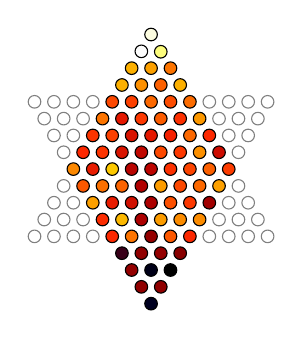
\begin{tikzpicture}
\filldraw [fill=C248] (0.000000,1.708957) circle (0.08); -- 501
\filldraw [fill=C255] (-0.123333,1.495337) circle (0.08); -- 518
\filldraw [fill=C220] (0.123333,1.490204) circle (0.08); -- 437
\filldraw [fill=C125] (-0.246667,1.281718) circle (0.08); -- 222
\filldraw [fill=C117] (0.000000,1.281718) circle (0.08); -- 203
\filldraw [fill=C95] (0.246667,1.281718) circle (0.08); -- 152
\filldraw [fill=C124] (-0.370000,1.068098) circle (0.08); -- 219
\filldraw [fill=C109] (-0.123333,1.068098) circle (0.08); -- 185
\filldraw [fill=C85] (0.123333,1.068098) circle (0.08); -- 131
\filldraw [fill=C124] (0.370000,1.068098) circle (0.08); -- 220
\draw [color=gray] (-1.480000,0.854478) circle (0.08); 
\draw [color=gray] (-1.233333,0.854478) circle (0.08); 
\draw [color=gray] (-0.986667,0.854478) circle (0.08); 
\draw [color=gray] (-0.740000,0.854478) circle (0.08); 
\filldraw [fill=C74] (-0.493333,0.854478) circle (0.08); -- 106
\filldraw [fill=C70] (-0.246667,0.854478) circle (0.08); -- 96
\filldraw [fill=C90] (0.000000,0.854478) circle (0.08); -- 141
\filldraw [fill=C77] (0.246667,0.854478) circle (0.08); -- 112
\filldraw [fill=C92] (0.493333,0.854478) circle (0.08); -- 146
\draw [color=gray] (0.740000,0.854478) circle (0.08); 
\draw [color=gray] (0.986667,0.854478) circle (0.08); 
\draw [color=gray] (1.233333,0.854478) circle (0.08); 
\draw [color=gray] (1.480000,0.854478) circle (0.08); 
\draw [color=gray] (-1.356667,0.640859) circle (0.08); 
\draw [color=gray] (-1.110000,0.640859) circle (0.08); 
\draw [color=gray] (-0.863333,0.640859) circle (0.08); 
\filldraw [fill=C95] (-0.616667,0.640859) circle (0.08); -- 154
\filldraw [fill=C51] (-0.370000,0.640859) circle (0.08); -- 54
\filldraw [fill=C67] (-0.123333,0.640859) circle (0.08); -- 90
\filldraw [fill=C84] (0.123333,0.640859) circle (0.08); -- 128
\filldraw [fill=C63] (0.370000,0.640859) circle (0.08); -- 81
\filldraw [fill=C113] (0.616667,0.640859) circle (0.08); -- 193
\draw [color=gray] (0.863333,0.640859) circle (0.08); 
\draw [color=gray] (1.110000,0.640859) circle (0.08); 
\draw [color=gray] (1.356667,0.640859) circle (0.08); 
\draw [color=gray] (-1.233333,0.427239) circle (0.08); 
\draw [color=gray] (-0.986667,0.427239) circle (0.08); 
\filldraw [fill=C64] (-0.740000,0.427239) circle (0.08); -- 83
\filldraw [fill=C71] (-0.493333,0.427239) circle (0.08); -- 98
\filldraw [fill=C48] (-0.246667,0.427239) circle (0.08); -- 46
\filldraw [fill=C51] (0.000000,0.427239) circle (0.08); -- 52
\filldraw [fill=C55] (0.246667,0.427239) circle (0.08); -- 62
\filldraw [fill=C90] (0.493333,0.427239) circle (0.08); -- 142
\filldraw [fill=C58] (0.740000,0.427239) circle (0.08); -- 69
\draw [color=gray] (0.986667,0.427239) circle (0.08); 
\draw [color=gray] (1.233333,0.427239) circle (0.08); 
\draw [color=gray] (-1.110000,0.213620) circle (0.08); 
\filldraw [fill=C58] (-0.863333,0.213620) circle (0.08); -- 69
\filldraw [fill=C64] (-0.616667,0.213620) circle (0.08); -- 82
\filldraw [fill=C48] (-0.370000,0.213620) circle (0.08); -- 47
\filldraw [fill=C42] (-0.123333,0.213620) circle (0.08); -- 33
\filldraw [fill=C75] (0.123333,0.213620) circle (0.08); -- 108
\filldraw [fill=C67] (0.370000,0.213620) circle (0.08); -- 89
\filldraw [fill=C110] (0.616667,0.213620) circle (0.08); -- 188
\filldraw [fill=C45] (0.863333,0.213620) circle (0.08); -- 40
\draw [color=gray] (1.110000,0.213620) circle (0.08); 
\filldraw [fill=C106] (-0.986667,0.000000) circle (0.08); -- 177
\filldraw [fill=C52] (-0.740000,0.000000) circle (0.08); -- 56
\filldraw [fill=C136] (-0.493333,0.000000) circle (0.08); -- 247
\filldraw [fill=C40] (-0.246667,0.000000) circle (0.08); -- 27
\filldraw [fill=C41] (0.000000,0.000000) circle (0.08); -- 31
\filldraw [fill=C62] (0.246667,0.000000) circle (0.08); -- 77
\filldraw [fill=C73] (0.493333,0.000000) circle (0.08); -- 102
\filldraw [fill=C85] (0.740000,0.000000) circle (0.08); -- 130
\filldraw [fill=C69] (0.986667,0.000000) circle (0.08); -- 94
\draw [color=gray] (-1.110000,-0.213620) circle (0.08); 
\filldraw [fill=C82] (-0.863333,-0.213620) circle (0.08); -- 123
\filldraw [fill=C94] (-0.616667,-0.213620) circle (0.08); -- 150
\filldraw [fill=C87] (-0.370000,-0.213620) circle (0.08); -- 135
\filldraw [fill=C38] (-0.123333,-0.213620) circle (0.08); -- 23
\filldraw [fill=C115] (0.123333,-0.213620) circle (0.08); -- 199
\filldraw [fill=C74] (0.370000,-0.213620) circle (0.08); -- 105
\filldraw [fill=C89] (0.616667,-0.213620) circle (0.08); -- 139
\filldraw [fill=C117] (0.863333,-0.213620) circle (0.08); -- 204
\draw [color=gray] (1.110000,-0.213620) circle (0.08); 
\draw [color=gray] (-1.233333,-0.427239) circle (0.08); 
\draw [color=gray] (-0.986667,-0.427239) circle (0.08); 
\filldraw [fill=C117] (-0.740000,-0.427239) circle (0.08); -- 203
\filldraw [fill=C52] (-0.493333,-0.427239) circle (0.08); -- 56
\filldraw [fill=C46] (-0.246667,-0.427239) circle (0.08); -- 41
\filldraw [fill=C37] (0.000000,-0.427239) circle (0.08); -- 22
\filldraw [fill=C79] (0.246667,-0.427239) circle (0.08); -- 117
\filldraw [fill=C67] (0.493333,-0.427239) circle (0.08); -- 90
\filldraw [fill=C34] (0.740000,-0.427239) circle (0.08); -- 15
\draw [color=gray] (0.986667,-0.427239) circle (0.08); 
\draw [color=gray] (1.233333,-0.427239) circle (0.08); 
\draw [color=gray] (-1.356667,-0.640859) circle (0.08); 
\draw [color=gray] (-1.110000,-0.640859) circle (0.08); 
\draw [color=gray] (-0.863333,-0.640859) circle (0.08); 
\filldraw [fill=C60] (-0.616667,-0.640859) circle (0.08); -- 73
\filldraw [fill=C128] (-0.370000,-0.640859) circle (0.08); -- 227
\filldraw [fill=C37] (-0.123333,-0.640859) circle (0.08); -- 21
\filldraw [fill=C114] (0.123333,-0.640859) circle (0.08); -- 196
\filldraw [fill=C107] (0.370000,-0.640859) circle (0.08); -- 181
\filldraw [fill=C108] (0.616667,-0.640859) circle (0.08); -- 183
\draw [color=gray] (0.863333,-0.640859) circle (0.08); 
\draw [color=gray] (1.110000,-0.640859) circle (0.08); 
\draw [color=gray] (1.356667,-0.640859) circle (0.08); 
\draw [color=gray] (-1.480000,-0.854478) circle (0.08); 
\draw [color=gray] (-1.233333,-0.854478) circle (0.08); 
\draw [color=gray] (-0.986667,-0.854478) circle (0.08); 
\draw [color=gray] (-0.740000,-0.854478) circle (0.08); 
\filldraw [fill=C59] (-0.493333,-0.854478) circle (0.08); -- 72
\filldraw [fill=C95] (-0.246667,-0.854478) circle (0.08); -- 153
\filldraw [fill=C30] (0.000000,-0.854478) circle (0.08); -- 5
\filldraw [fill=C82] (0.246667,-0.854478) circle (0.08); -- 124
\filldraw [fill=C59] (0.493333,-0.854478) circle (0.08); -- 72
\draw [color=gray] (0.740000,-0.854478) circle (0.08); 
\draw [color=gray] (0.986667,-0.854478) circle (0.08); 
\draw [color=gray] (1.233333,-0.854478) circle (0.08); 
\draw [color=gray] (1.480000,-0.854478) circle (0.08); 
\filldraw [fill=C14] (-0.370000,-1.068099) circle (0.08); -- -32
\filldraw [fill=C29] (-0.123333,-1.068099) circle (0.08); -- 3
\filldraw [fill=C30] (0.123333,-1.068099) circle (0.08); -- 5
\filldraw [fill=C26] (0.370000,-1.068099) circle (0.08); -- -3
\filldraw [fill=C30] (-0.246667,-1.281718) circle (0.08); -- 5
\filldraw [fill=C1] (0.000000,-1.281718) circle (0.08); -- -61
\filldraw [fill=C0] (0.246667,-1.281718) circle (0.08); -- -62
\filldraw [fill=C29] (-0.123333,-1.495338) circle (0.08); -- 2
\filldraw [fill=C28] (0.123333,-1.495338) circle (0.08); -- 0
\filldraw [fill=C4] (0.000000,-1.708957) circle (0.08); -- -53
\end{tikzpicture}

\caption{This individual from generation 7822 had a fitness of
  $427.4$, the highest of all individuals generated. When tested by
  the genetic algorithm it won in an average of only $500-427.4=72.6$
  moves.}
\label{genpop7822}
\end{figure}

\begin{figure}
\centering
\definecolor{C0}{rgb}{0.000000,0.000000,0.000000}
\definecolor{C1}{rgb}{0.000000,0.000000,0.094118}
\definecolor{C2}{rgb}{0.000000,0.000000,0.094118}
\definecolor{C3}{rgb}{0.000000,0.000000,0.109804}
\definecolor{C4}{rgb}{0.000000,0.000000,0.125490}
\definecolor{C5}{rgb}{0.000000,0.000000,0.125490}
\definecolor{C6}{rgb}{0.000000,0.000000,0.141176}
\definecolor{C7}{rgb}{0.000000,0.000000,0.156863}
\definecolor{C8}{rgb}{0.031373,0.000000,0.156863}
\definecolor{C9}{rgb}{0.062745,0.000000,0.141176}
\definecolor{C10}{rgb}{0.094118,0.000000,0.141176}
\definecolor{C11}{rgb}{0.125490,0.000000,0.125490}
\definecolor{C12}{rgb}{0.156863,0.000000,0.109804}
\definecolor{C13}{rgb}{0.188235,0.000000,0.109804}
\definecolor{C14}{rgb}{0.219608,0.000000,0.094118}
\definecolor{C15}{rgb}{0.250980,0.000000,0.078431}
\definecolor{C16}{rgb}{0.282353,0.000000,0.078431}
\definecolor{C17}{rgb}{0.313725,0.000000,0.062745}
\definecolor{C18}{rgb}{0.345098,0.000000,0.062745}
\definecolor{C19}{rgb}{0.376471,0.000000,0.047059}
\definecolor{C20}{rgb}{0.407843,0.000000,0.031373}
\definecolor{C21}{rgb}{0.439216,0.000000,0.031373}
\definecolor{C22}{rgb}{0.470588,0.000000,0.015686}
\definecolor{C23}{rgb}{0.501961,0.000000,0.000000}
\definecolor{C24}{rgb}{0.501961,0.000000,0.000000}
\definecolor{C25}{rgb}{0.517647,0.000000,0.000000}
\definecolor{C26}{rgb}{0.533333,0.000000,0.000000}
\definecolor{C27}{rgb}{0.549020,0.000000,0.000000}
\definecolor{C28}{rgb}{0.564706,0.000000,0.000000}
\definecolor{C29}{rgb}{0.564706,0.000000,0.000000}
\definecolor{C30}{rgb}{0.580392,0.000000,0.000000}
\definecolor{C31}{rgb}{0.596078,0.000000,0.000000}
\definecolor{C32}{rgb}{0.611765,0.000000,0.000000}
\definecolor{C33}{rgb}{0.627451,0.000000,0.000000}
\definecolor{C34}{rgb}{0.627451,0.000000,0.000000}
\definecolor{C35}{rgb}{0.643137,0.000000,0.000000}
\definecolor{C36}{rgb}{0.658824,0.000000,0.000000}
\definecolor{C37}{rgb}{0.674510,0.000000,0.000000}
\definecolor{C38}{rgb}{0.690196,0.000000,0.000000}
\definecolor{C39}{rgb}{0.705882,0.000000,0.000000}
\definecolor{C40}{rgb}{0.721569,0.015686,0.000000}
\definecolor{C41}{rgb}{0.737255,0.015686,0.000000}
\definecolor{C42}{rgb}{0.752941,0.031373,0.000000}
\definecolor{C43}{rgb}{0.768627,0.031373,0.000000}
\definecolor{C44}{rgb}{0.784314,0.047059,0.000000}
\definecolor{C45}{rgb}{0.800000,0.047059,0.000000}
\definecolor{C46}{rgb}{0.815686,0.062745,0.000000}
\definecolor{C47}{rgb}{0.831373,0.062745,0.000000}
\definecolor{C48}{rgb}{0.847059,0.078431,0.000000}
\definecolor{C49}{rgb}{0.862745,0.078431,0.000000}
\definecolor{C50}{rgb}{0.878431,0.094118,0.000000}
\definecolor{C51}{rgb}{0.894118,0.094118,0.000000}
\definecolor{C52}{rgb}{0.909804,0.109804,0.000000}
\definecolor{C53}{rgb}{0.925490,0.109804,0.000000}
\definecolor{C54}{rgb}{0.941176,0.125490,0.000000}
\definecolor{C55}{rgb}{0.956863,0.125490,0.000000}
\definecolor{C56}{rgb}{0.988235,0.141176,0.000000}
\definecolor{C57}{rgb}{0.988235,0.141176,0.000000}
\definecolor{C58}{rgb}{0.988235,0.156863,0.000000}
\definecolor{C59}{rgb}{0.988235,0.156863,0.000000}
\definecolor{C60}{rgb}{0.988235,0.172549,0.000000}
\definecolor{C61}{rgb}{0.988235,0.172549,0.000000}
\definecolor{C62}{rgb}{0.988235,0.188235,0.000000}
\definecolor{C63}{rgb}{0.988235,0.188235,0.000000}
\definecolor{C64}{rgb}{0.988235,0.203922,0.000000}
\definecolor{C65}{rgb}{0.988235,0.203922,0.000000}
\definecolor{C66}{rgb}{0.988235,0.219608,0.000000}
\definecolor{C67}{rgb}{0.988235,0.219608,0.000000}
\definecolor{C68}{rgb}{0.988235,0.235294,0.000000}
\definecolor{C69}{rgb}{0.988235,0.235294,0.000000}
\definecolor{C70}{rgb}{0.988235,0.250980,0.000000}
\definecolor{C71}{rgb}{0.988235,0.250980,0.000000}
\definecolor{C72}{rgb}{0.988235,0.266667,0.000000}
\definecolor{C73}{rgb}{0.988235,0.266667,0.000000}
\definecolor{C74}{rgb}{0.988235,0.282353,0.000000}
\definecolor{C75}{rgb}{0.988235,0.282353,0.000000}
\definecolor{C76}{rgb}{0.988235,0.298039,0.000000}
\definecolor{C77}{rgb}{0.988235,0.298039,0.000000}
\definecolor{C78}{rgb}{0.988235,0.313725,0.000000}
\definecolor{C79}{rgb}{0.988235,0.313725,0.000000}
\definecolor{C80}{rgb}{0.988235,0.329412,0.000000}
\definecolor{C81}{rgb}{0.988235,0.329412,0.000000}
\definecolor{C82}{rgb}{0.988235,0.345098,0.000000}
\definecolor{C83}{rgb}{0.988235,0.345098,0.000000}
\definecolor{C84}{rgb}{0.988235,0.360784,0.000000}
\definecolor{C85}{rgb}{0.988235,0.376471,0.000000}
\definecolor{C86}{rgb}{0.988235,0.376471,0.000000}
\definecolor{C87}{rgb}{0.988235,0.392157,0.000000}
\definecolor{C88}{rgb}{0.988235,0.392157,0.000000}
\definecolor{C89}{rgb}{0.988235,0.407843,0.000000}
\definecolor{C90}{rgb}{0.988235,0.407843,0.000000}
\definecolor{C91}{rgb}{0.988235,0.423529,0.000000}
\definecolor{C92}{rgb}{0.988235,0.423529,0.000000}
\definecolor{C93}{rgb}{0.988235,0.439216,0.000000}
\definecolor{C94}{rgb}{0.988235,0.439216,0.000000}
\definecolor{C95}{rgb}{0.988235,0.454902,0.000000}
\definecolor{C96}{rgb}{0.988235,0.454902,0.000000}
\definecolor{C97}{rgb}{0.988235,0.470588,0.000000}
\definecolor{C98}{rgb}{0.988235,0.470588,0.000000}
\definecolor{C99}{rgb}{0.988235,0.486275,0.000000}
\definecolor{C100}{rgb}{0.988235,0.486275,0.000000}
\definecolor{C101}{rgb}{0.988235,0.501961,0.000000}
\definecolor{C102}{rgb}{0.988235,0.501961,0.000000}
\definecolor{C103}{rgb}{0.988235,0.517647,0.000000}
\definecolor{C104}{rgb}{0.988235,0.517647,0.000000}
\definecolor{C105}{rgb}{0.988235,0.533333,0.000000}
\definecolor{C106}{rgb}{0.988235,0.533333,0.000000}
\definecolor{C107}{rgb}{0.988235,0.549020,0.000000}
\definecolor{C108}{rgb}{0.988235,0.549020,0.000000}
\definecolor{C109}{rgb}{0.988235,0.564706,0.000000}
\definecolor{C110}{rgb}{0.988235,0.564706,0.000000}
\definecolor{C111}{rgb}{0.988235,0.580392,0.000000}
\definecolor{C112}{rgb}{0.988235,0.596078,0.000000}
\definecolor{C113}{rgb}{0.988235,0.596078,0.000000}
\definecolor{C114}{rgb}{0.988235,0.611765,0.000000}
\definecolor{C115}{rgb}{0.988235,0.611765,0.000000}
\definecolor{C116}{rgb}{0.988235,0.627451,0.000000}
\definecolor{C117}{rgb}{0.988235,0.627451,0.000000}
\definecolor{C118}{rgb}{0.988235,0.643137,0.000000}
\definecolor{C119}{rgb}{0.988235,0.643137,0.000000}
\definecolor{C120}{rgb}{0.988235,0.658824,0.000000}
\definecolor{C121}{rgb}{0.988235,0.658824,0.000000}
\definecolor{C122}{rgb}{0.988235,0.674510,0.000000}
\definecolor{C123}{rgb}{0.988235,0.674510,0.000000}
\definecolor{C124}{rgb}{0.988235,0.690196,0.000000}
\definecolor{C125}{rgb}{0.988235,0.690196,0.000000}
\definecolor{C126}{rgb}{0.988235,0.705882,0.000000}
\definecolor{C127}{rgb}{0.988235,0.705882,0.000000}
\definecolor{C128}{rgb}{0.988235,0.721569,0.000000}
\definecolor{C129}{rgb}{0.988235,0.721569,0.000000}
\definecolor{C130}{rgb}{0.988235,0.737255,0.000000}
\definecolor{C131}{rgb}{0.988235,0.737255,0.000000}
\definecolor{C132}{rgb}{0.988235,0.752941,0.000000}
\definecolor{C133}{rgb}{0.988235,0.752941,0.000000}
\definecolor{C134}{rgb}{0.988235,0.768627,0.000000}
\definecolor{C135}{rgb}{0.988235,0.768627,0.000000}
\definecolor{C136}{rgb}{0.988235,0.784314,0.000000}
\definecolor{C137}{rgb}{0.988235,0.784314,0.000000}
\definecolor{C138}{rgb}{0.988235,0.800000,0.000000}
\definecolor{C139}{rgb}{0.988235,0.815686,0.000000}
\definecolor{C140}{rgb}{0.988235,0.815686,0.000000}
\definecolor{C141}{rgb}{0.988235,0.815686,0.000000}
\definecolor{C142}{rgb}{0.988235,0.815686,0.000000}
\definecolor{C143}{rgb}{0.988235,0.815686,0.000000}
\definecolor{C144}{rgb}{0.988235,0.831373,0.000000}
\definecolor{C145}{rgb}{0.988235,0.831373,0.000000}
\definecolor{C146}{rgb}{0.988235,0.831373,0.000000}
\definecolor{C147}{rgb}{0.988235,0.831373,0.000000}
\definecolor{C148}{rgb}{0.988235,0.847059,0.000000}
\definecolor{C149}{rgb}{0.988235,0.847059,0.000000}
\definecolor{C150}{rgb}{0.988235,0.847059,0.000000}
\definecolor{C151}{rgb}{0.988235,0.847059,0.000000}
\definecolor{C152}{rgb}{0.988235,0.847059,0.000000}
\definecolor{C153}{rgb}{0.988235,0.862745,0.000000}
\definecolor{C154}{rgb}{0.988235,0.862745,0.000000}
\definecolor{C155}{rgb}{0.988235,0.862745,0.000000}
\definecolor{C156}{rgb}{0.988235,0.862745,0.000000}
\definecolor{C157}{rgb}{0.988235,0.878431,0.000000}
\definecolor{C158}{rgb}{0.988235,0.878431,0.000000}
\definecolor{C159}{rgb}{0.988235,0.878431,0.000000}
\definecolor{C160}{rgb}{0.988235,0.878431,0.000000}
\definecolor{C161}{rgb}{0.988235,0.894118,0.000000}
\definecolor{C162}{rgb}{0.988235,0.894118,0.000000}
\definecolor{C163}{rgb}{0.988235,0.894118,0.000000}
\definecolor{C164}{rgb}{0.988235,0.894118,0.000000}
\definecolor{C165}{rgb}{0.988235,0.894118,0.000000}
\definecolor{C166}{rgb}{0.988235,0.909804,0.000000}
\definecolor{C167}{rgb}{0.988235,0.909804,0.000000}
\definecolor{C168}{rgb}{0.988235,0.909804,0.000000}
\definecolor{C169}{rgb}{0.988235,0.909804,0.000000}
\definecolor{C170}{rgb}{0.988235,0.925490,0.000000}
\definecolor{C171}{rgb}{0.988235,0.925490,0.000000}
\definecolor{C172}{rgb}{0.988235,0.925490,0.000000}
\definecolor{C173}{rgb}{0.988235,0.925490,0.000000}
\definecolor{C174}{rgb}{0.988235,0.941176,0.000000}
\definecolor{C175}{rgb}{0.988235,0.941176,0.000000}
\definecolor{C176}{rgb}{0.988235,0.941176,0.000000}
\definecolor{C177}{rgb}{0.988235,0.941176,0.000000}
\definecolor{C178}{rgb}{0.988235,0.941176,0.000000}
\definecolor{C179}{rgb}{0.988235,0.956863,0.000000}
\definecolor{C180}{rgb}{0.988235,0.956863,0.000000}
\definecolor{C181}{rgb}{0.988235,0.956863,0.000000}
\definecolor{C182}{rgb}{0.988235,0.956863,0.000000}
\definecolor{C183}{rgb}{0.988235,0.972549,0.000000}
\definecolor{C184}{rgb}{0.988235,0.972549,0.000000}
\definecolor{C185}{rgb}{0.988235,0.972549,0.000000}
\definecolor{C186}{rgb}{0.988235,0.972549,0.000000}
\definecolor{C187}{rgb}{0.988235,0.988235,0.000000}
\definecolor{C188}{rgb}{0.988235,0.988235,0.015686}
\definecolor{C189}{rgb}{0.988235,0.988235,0.031373}
\definecolor{C190}{rgb}{0.988235,0.988235,0.047059}
\definecolor{C191}{rgb}{0.988235,0.988235,0.062745}
\definecolor{C192}{rgb}{0.988235,0.988235,0.078431}
\definecolor{C193}{rgb}{0.988235,0.988235,0.094118}
\definecolor{C194}{rgb}{0.988235,0.988235,0.109804}
\definecolor{C195}{rgb}{0.988235,0.988235,0.125490}
\definecolor{C196}{rgb}{0.988235,0.988235,0.141176}
\definecolor{C197}{rgb}{0.988235,0.988235,0.156863}
\definecolor{C198}{rgb}{0.988235,0.988235,0.156863}
\definecolor{C199}{rgb}{0.988235,0.988235,0.172549}
\definecolor{C200}{rgb}{0.988235,0.988235,0.188235}
\definecolor{C201}{rgb}{0.988235,0.988235,0.203922}
\definecolor{C202}{rgb}{0.988235,0.988235,0.219608}
\definecolor{C203}{rgb}{0.988235,0.988235,0.235294}
\definecolor{C204}{rgb}{0.988235,0.988235,0.250980}
\definecolor{C205}{rgb}{0.988235,0.988235,0.266667}
\definecolor{C206}{rgb}{0.988235,0.988235,0.282353}
\definecolor{C207}{rgb}{0.988235,0.988235,0.298039}
\definecolor{C208}{rgb}{0.988235,0.988235,0.313725}
\definecolor{C209}{rgb}{0.988235,0.988235,0.329412}
\definecolor{C210}{rgb}{0.988235,0.988235,0.329412}
\definecolor{C211}{rgb}{0.988235,0.988235,0.345098}
\definecolor{C212}{rgb}{0.988235,0.988235,0.360784}
\definecolor{C213}{rgb}{0.988235,0.988235,0.376471}
\definecolor{C214}{rgb}{0.988235,0.988235,0.392157}
\definecolor{C215}{rgb}{0.988235,0.988235,0.407843}
\definecolor{C216}{rgb}{0.988235,0.988235,0.423529}
\definecolor{C217}{rgb}{0.988235,0.988235,0.439216}
\definecolor{C218}{rgb}{0.988235,0.988235,0.454902}
\definecolor{C219}{rgb}{0.988235,0.988235,0.470588}
\definecolor{C220}{rgb}{0.988235,0.988235,0.486275}
\definecolor{C221}{rgb}{0.988235,0.988235,0.486275}
\definecolor{C222}{rgb}{0.988235,0.988235,0.501961}
\definecolor{C223}{rgb}{0.988235,0.988235,0.517647}
\definecolor{C224}{rgb}{0.988235,0.988235,0.533333}
\definecolor{C225}{rgb}{0.988235,0.988235,0.549020}
\definecolor{C226}{rgb}{0.988235,0.988235,0.564706}
\definecolor{C227}{rgb}{0.988235,0.988235,0.580392}
\definecolor{C228}{rgb}{0.988235,0.988235,0.596078}
\definecolor{C229}{rgb}{0.988235,0.988235,0.611765}
\definecolor{C230}{rgb}{0.988235,0.988235,0.627451}
\definecolor{C231}{rgb}{0.988235,0.988235,0.643137}
\definecolor{C232}{rgb}{0.988235,0.988235,0.658824}
\definecolor{C233}{rgb}{0.988235,0.988235,0.658824}
\definecolor{C234}{rgb}{0.988235,0.988235,0.674510}
\definecolor{C235}{rgb}{0.988235,0.988235,0.690196}
\definecolor{C236}{rgb}{0.988235,0.988235,0.705882}
\definecolor{C237}{rgb}{0.988235,0.988235,0.721569}
\definecolor{C238}{rgb}{0.988235,0.988235,0.737255}
\definecolor{C239}{rgb}{0.988235,0.988235,0.752941}
\definecolor{C240}{rgb}{0.988235,0.988235,0.768627}
\definecolor{C241}{rgb}{0.988235,0.988235,0.784314}
\definecolor{C242}{rgb}{0.988235,0.988235,0.800000}
\definecolor{C243}{rgb}{0.988235,0.988235,0.815686}
\definecolor{C244}{rgb}{0.988235,0.988235,0.815686}
\definecolor{C245}{rgb}{0.988235,0.988235,0.831373}
\definecolor{C246}{rgb}{0.988235,0.988235,0.847059}
\definecolor{C247}{rgb}{0.988235,0.988235,0.862745}
\definecolor{C248}{rgb}{0.988235,0.988235,0.878431}
\definecolor{C249}{rgb}{0.988235,0.988235,0.894118}
\definecolor{C250}{rgb}{0.988235,0.988235,0.909804}
\definecolor{C251}{rgb}{0.988235,0.988235,0.925490}
\definecolor{C252}{rgb}{0.988235,0.988235,0.941176}
\definecolor{C253}{rgb}{0.988235,0.988235,0.956863}
\definecolor{C254}{rgb}{0.988235,0.988235,0.972549}
\definecolor{C255}{rgb}{0.988235,0.988235,0.988235}

%% vec = (154, 17, 2, 22, 519, 91, 54, 98, 123, 45, 61, 32, 60, 23, 120, 78, 91, 10, 17, 177, 72, 492, 514, 46, 138, 68, 133, 193, 77, 22, 181, 9, 5, 33, 147, 177, 182, 23, 203, 204, 202, 174, 100, 109, 2, 51, 47, 204, 24, 108, 132, 66, 65, 12, 98, 213, 191, 202, 237, 64, 123, 237, 69, 44, 61, 119, 185, 161, 8, 103, 47, 193, 157, 183, 106, 93, 101, 179, 170, 110, 5, 102, 183, 191, 109, 78, 157, 202, 41, 63, 74, 66, 113, 77, 158, 109, 10, 6, 89, 17, 70, 185, 144, 125, 60, 118, 82, 183, 44, 202, 55, 131, 111, 8, 123, 216, 41, 120, 24, 15, 53, 59, 52, 164, 105, 61, 31, 236, 33, 178, 43, 146, 39, 139, 55, 161, 151, 110, 63, 165, 102, 69, 188, 25, 23, 27, 197, 48, 77, 224, 205, 81, 151, 10, 20, 42, 1, 160, 107, 178, 104, 19, 190, 91, 140, 163, 31, 189, 69, 155, 117, 142, 61, 57, 139, 131, 91, 152, 16, 102, 97, 30, 185, 121, 190, 81, 162, 89, 149, 31, 148, 93, 119, 102, 81, 26, 16, 26, 39, 205, 33, 214, 90, 144, 66, 223, 112, 186, 183, 128, 134, 68, 43, 14, 52, 92, 144, 9, 154, 179, 139, 173, 37, 91, 110, 74, 70, 124, 5, 114, 5, -10, -27, -5, 10, 100, 16, 30, 78, 144, 126, 75, 80, 159, 8, 2, 141, 171, 4, 0, -1, 47, 27, 54, 3, 2, 74, 60, 115, 18, 16, 67, 31, 11, 188, 158, 0, -59, 139, 99, 62, 111, 137, 164, 163, 112, 135, 132, 174, 54, 12, 91, 149, 22, -12, 85, 73, 10, 164)
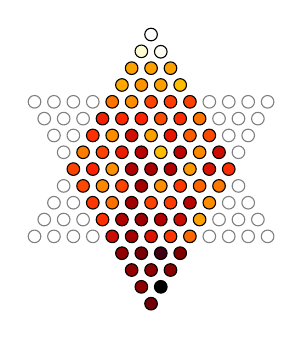
\begin{tikzpicture}
\filldraw [fill=C255] (0.000000,1.708957) circle (0.08); -- 519
\filldraw [fill=C244] (-0.123333,1.495337) circle (0.08); -- 492
\filldraw [fill=C253] (0.123333,1.490204) circle (0.08); -- 514
\filldraw [fill=C116] (-0.246667,1.281718) circle (0.08); -- 203
\filldraw [fill=C117] (0.000000,1.281718) circle (0.08); -- 204
\filldraw [fill=C116] (0.246667,1.281718) circle (0.08); -- 202
\filldraw [fill=C120] (-0.370000,1.068098) circle (0.08); -- 213
\filldraw [fill=C111] (-0.123333,1.068098) circle (0.08); -- 191
\filldraw [fill=C116] (0.123333,1.068098) circle (0.08); -- 202
\filldraw [fill=C131] (0.370000,1.068098) circle (0.08); -- 237
\draw [color=gray] (-1.480000,0.854478) circle (0.08); 
\draw [color=gray] (-1.233333,0.854478) circle (0.08); 
\draw [color=gray] (-0.986667,0.854478) circle (0.08); 
\draw [color=gray] (-0.740000,0.854478) circle (0.08); 
\filldraw [fill=C96] (-0.493333,0.854478) circle (0.08); -- 157
\filldraw [fill=C107] (-0.246667,0.854478) circle (0.08); -- 183
\filldraw [fill=C73] (0.000000,0.854478) circle (0.08); -- 106
\filldraw [fill=C68] (0.246667,0.854478) circle (0.08); -- 93
\filldraw [fill=C71] (0.493333,0.854478) circle (0.08); -- 101
\draw [color=gray] (0.740000,0.854478) circle (0.08); 
\draw [color=gray] (0.986667,0.854478) circle (0.08); 
\draw [color=gray] (1.233333,0.854478) circle (0.08); 
\draw [color=gray] (1.480000,0.854478) circle (0.08); 
\draw [color=gray] (-1.356667,0.640859) circle (0.08); 
\draw [color=gray] (-1.110000,0.640859) circle (0.08); 
\draw [color=gray] (-0.863333,0.640859) circle (0.08); 
\filldraw [fill=C54] (-0.616667,0.640859) circle (0.08); -- 63
\filldraw [fill=C59] (-0.370000,0.640859) circle (0.08); -- 74
\filldraw [fill=C56] (-0.123333,0.640859) circle (0.08); -- 66
\filldraw [fill=C76] (0.123333,0.640859) circle (0.08); -- 113
\filldraw [fill=C60] (0.370000,0.640859) circle (0.08); -- 77
\filldraw [fill=C96] (0.616667,0.640859) circle (0.08); -- 158
\draw [color=gray] (0.863333,0.640859) circle (0.08); 
\draw [color=gray] (1.110000,0.640859) circle (0.08); 
\draw [color=gray] (1.356667,0.640859) circle (0.08); 
\draw [color=gray] (-1.233333,0.427239) circle (0.08); 
\draw [color=gray] (-0.986667,0.427239) circle (0.08); 
\filldraw [fill=C63] (-0.740000,0.427239) circle (0.08); -- 82
\filldraw [fill=C107] (-0.493333,0.427239) circle (0.08); -- 183
\filldraw [fill=C46] (-0.246667,0.427239) circle (0.08); -- 44
\filldraw [fill=C116] (0.000000,0.427239) circle (0.08); -- 202
\filldraw [fill=C51] (0.246667,0.427239) circle (0.08); -- 55
\filldraw [fill=C84] (0.493333,0.427239) circle (0.08); -- 131
\filldraw [fill=C75] (0.740000,0.427239) circle (0.08); -- 111
\draw [color=gray] (0.986667,0.427239) circle (0.08); 
\draw [color=gray] (1.233333,0.427239) circle (0.08); 
\draw [color=gray] (-1.110000,0.213620) circle (0.08); 
\filldraw [fill=C99] (-0.863333,0.213620) circle (0.08); -- 164
\filldraw [fill=C73] (-0.616667,0.213620) circle (0.08); -- 105
\filldraw [fill=C53] (-0.370000,0.213620) circle (0.08); -- 61
\filldraw [fill=C40] (-0.123333,0.213620) circle (0.08); -- 31
\filldraw [fill=C131] (0.123333,0.213620) circle (0.08); -- 236
\filldraw [fill=C41] (0.370000,0.213620) circle (0.08); -- 33
\filldraw [fill=C105] (0.616667,0.213620) circle (0.08); -- 178
\filldraw [fill=C45] (0.863333,0.213620) circle (0.08); -- 43
\draw [color=gray] (1.110000,0.213620) circle (0.08); 
\filldraw [fill=C72] (-0.986667,0.000000) circle (0.08); -- 102
\filldraw [fill=C57] (-0.740000,0.000000) circle (0.08); -- 69
\filldraw [fill=C109] (-0.493333,0.000000) circle (0.08); -- 188
\filldraw [fill=C38] (-0.246667,0.000000) circle (0.08); -- 25
\filldraw [fill=C37] (0.000000,0.000000) circle (0.08); -- 23
\filldraw [fill=C38] (0.246667,0.000000) circle (0.08); -- 27
\filldraw [fill=C113] (0.493333,0.000000) circle (0.08); -- 197
\filldraw [fill=C48] (0.740000,0.000000) circle (0.08); -- 48
\filldraw [fill=C60] (0.986667,0.000000) circle (0.08); -- 77
\draw [color=gray] (-1.110000,-0.213620) circle (0.08); 
\filldraw [fill=C74] (-0.863333,-0.213620) circle (0.08); -- 107
\filldraw [fill=C105] (-0.616667,-0.213620) circle (0.08); -- 178
\filldraw [fill=C72] (-0.370000,-0.213620) circle (0.08); -- 104
\filldraw [fill=C35] (-0.123333,-0.213620) circle (0.08); -- 19
\filldraw [fill=C110] (0.123333,-0.213620) circle (0.08); -- 190
\filldraw [fill=C67] (0.370000,-0.213620) circle (0.08); -- 91
\filldraw [fill=C88] (0.616667,-0.213620) circle (0.08); -- 140
\filldraw [fill=C98] (0.863333,-0.213620) circle (0.08); -- 163
\draw [color=gray] (1.110000,-0.213620) circle (0.08); 
\draw [color=gray] (-1.233333,-0.427239) circle (0.08); 
\draw [color=gray] (-0.986667,-0.427239) circle (0.08); 
\filldraw [fill=C67] (-0.740000,-0.427239) circle (0.08); -- 91
\filldraw [fill=C94] (-0.493333,-0.427239) circle (0.08); -- 152
\filldraw [fill=C34] (-0.246667,-0.427239) circle (0.08); -- 16
\filldraw [fill=C72] (0.000000,-0.427239) circle (0.08); -- 102
\filldraw [fill=C69] (0.246667,-0.427239) circle (0.08); -- 97
\filldraw [fill=C40] (0.493333,-0.427239) circle (0.08); -- 30
\filldraw [fill=C108] (0.740000,-0.427239) circle (0.08); -- 185
\draw [color=gray] (0.986667,-0.427239) circle (0.08); 
\draw [color=gray] (1.233333,-0.427239) circle (0.08); 
\draw [color=gray] (-1.356667,-0.640859) circle (0.08); 
\draw [color=gray] (-1.110000,-0.640859) circle (0.08); 
\draw [color=gray] (-0.863333,-0.640859) circle (0.08); 
\filldraw [fill=C62] (-0.616667,-0.640859) circle (0.08); -- 81
\filldraw [fill=C38] (-0.370000,-0.640859) circle (0.08); -- 26
\filldraw [fill=C34] (-0.123333,-0.640859) circle (0.08); -- 16
\filldraw [fill=C38] (0.123333,-0.640859) circle (0.08); -- 26
\filldraw [fill=C44] (0.370000,-0.640859) circle (0.08); -- 39
\filldraw [fill=C117] (0.616667,-0.640859) circle (0.08); -- 205
\draw [color=gray] (0.863333,-0.640859) circle (0.08); 
\draw [color=gray] (1.110000,-0.640859) circle (0.08); 
\draw [color=gray] (1.356667,-0.640859) circle (0.08); 
\draw [color=gray] (-1.480000,-0.854478) circle (0.08); 
\draw [color=gray] (-1.233333,-0.854478) circle (0.08); 
\draw [color=gray] (-0.986667,-0.854478) circle (0.08); 
\draw [color=gray] (-0.740000,-0.854478) circle (0.08); 
\filldraw [fill=C45] (-0.493333,-0.854478) circle (0.08); -- 43
\filldraw [fill=C33] (-0.246667,-0.854478) circle (0.08); -- 14
\filldraw [fill=C49] (0.000000,-0.854478) circle (0.08); -- 52
\filldraw [fill=C67] (0.246667,-0.854478) circle (0.08); -- 92
\filldraw [fill=C90] (0.493333,-0.854478) circle (0.08); -- 144
\draw [color=gray] (0.740000,-0.854478) circle (0.08); 
\draw [color=gray] (0.986667,-0.854478) circle (0.08); 
\draw [color=gray] (1.233333,-0.854478) circle (0.08); 
\draw [color=gray] (1.480000,-0.854478) circle (0.08); 
\filldraw [fill=C29] (-0.370000,-1.068099) circle (0.08); -- 5
\filldraw [fill=C22] (-0.123333,-1.068099) circle (0.08); -- -10
\filldraw [fill=C15] (0.123333,-1.068099) circle (0.08); -- -27
\filldraw [fill=C24] (0.370000,-1.068099) circle (0.08); -- -5
\filldraw [fill=C28] (-0.246667,-1.281718) circle (0.08); -- 4
\filldraw [fill=C27] (0.000000,-1.281718) circle (0.08); -- 0
\filldraw [fill=C26] (0.246667,-1.281718) circle (0.08); -- -1
\filldraw [fill=C27] (-0.123333,-1.495338) circle (0.08); -- 0
\filldraw [fill=C0] (0.123333,-1.495338) circle (0.08); -- -59
\filldraw [fill=C21] (0.000000,-1.708957) circle (0.08); -- -12
\end{tikzpicture}

\caption{We extended the algorithm to simulate three-player games.
  This individual comes from population 3594 in such a run. It had
  $99.2\%$ wins and a fitness of $393.4$.}
\label{gen3pop3594}
\end{figure}

